% !TEX root = ../eval.tex

\section{Results}%
\label{sec:results}

The main outcome variables in my analysis are ``discretionary spend'', defined
as spend transactions over which users likely have a lot of control, and
``net-inflows into savings-accounts'', defined as the difference between
inflows into and outflows from all of a user's savings accounts.\footnote{I do
    not include gasoline expenses in discretionary spend because many people
    use their car to commute to work so that it is unclear how much of these
    expenses is discretionary. When creating discretionary spend subgroups, I
    classify transactions tagged by MDB as ``entertainment'' as ``other''
    discretionary spend, since many such transactions are purchses with Amazon,
    which we cannot precisely classify. A list of transaction tags used to
    identify discretionary spend transactions and the code used create the
    variable are available on Github
    (\href{https://github.com/fabiangunzinger/mdb_eval/blob/f31bfcd7a330188cdd27968d41957ebf5b454099/src/data/aggregators.py#L389}{\faGithub}.
    To capture only user-generated savings-account flows and not interest
    payments and similar automated transactions I include only transaction with
an absolute value of \pounds5 or higher. The code used to calculate savings
account flows is also available on Github
(\href{https://github.com/fabiangunzinger/mdb_eval/blob/f31bfcd7a330188cdd27968d41957ebf5b454099/src/data/aggregators.py#L89}{\faGithub}.}


\subsection{Main results}%
\label{sub:main_results}

\begin{itemize}

    \item Figure~\ref{fig:main_results} shows the effect of app use on monthly
        discretionary spend (top row) and monthly net-inflows into savings
        accounts (bottom row) under the unconditional (left column) and
        conditional (right column) parallel trends assumptions.

    \item Estimates are group-time average treatment effects aggregated by time
        since treatment exposure.

    \item All results are presented with a uniform 95\% confidence band, based
        on bootstrapped standard errors clustered at the user level that also
        account for autocorrelation in the data.\footnote{A uniform 95\%
            confidence band accounts for multiple hypothesis testing in that it
            is constructed such that \textit{all} shown coefficients cover
            their corresponding true value 95 percent of the time. In contrast,
            a more commonly used pointwise 95\% confidence band is constructed
        such that the confidence interval for each parameter covers the true
    parameter 95 percent of the time.}

    \item Conditional results use the doubly-robust estimator discussed in the
        methods section.

    \item We can see that discretionary spend falls by between \pounds100 and
        \pounds150 per month once users start using the app, depending on the
        parallel trends assumption used. Given that average
        monthly discretionary spend is about \pounds860 (see
        Table~\ref{tab:sumstats}), this corresponds to a drop in discretionary
        spend of about 11-17 percent, which is substantial.

    \item These results are in line with those found in \citet{levi2020mind},
        which find a 11.6 percent reduction in discretionary spend following
        the use of an aggregator app.

    \item Conditional parallel trends are important in contexts when (i) there
        are covariate specific trends in outcome paths and (ii) the
        distribution of covariates differs between groups. (E.g. people who
        sign up to job training differ from those who don't and job outcomes
        depend on these covariates)

        Actually, for my here, cov distr between treatment and control differs
        only if early users are different from later ones.

    \item  Given that our comparison group is the set of
        ``not-yet-treated`` users rather than a set of ``never-treated`` users,
        the relatively small difference in results is as expected.

    \item At the same time, we would have expected there to be some difference.
        If we discretionary spend is a constant fraction of income and total
        spend, then we would expect parallel trends to hold only for groups
        with the same income and total monthly spend. Similarly, if we think
        that the average spend per account observed is constant, then parallel
        trends hold only for users with the same number of observed accounts
        (if we think of active accounts as observed accounts).

    \item In contrast to discretionary spend, net-inflows into savings accounts
        do not change once users start using the app. The wide confidence
        bands reflect the large variation in net-inflows already seen in
        Table~\ref{tab:sumstats}.

    \item Results indicate that parallel trend assumption might not hold. So we
        should interpret these result with some
        caution.\footnote{In future work, I plan to use the approach introduced
            by \citet{rambachan2022more} to test how sensitive my results are
        to deviations from parallel trends.}


\end{itemize}


\begin{figure}[H]
    \centering 
    \caption{Main results}
    \label{fig:main_results}
    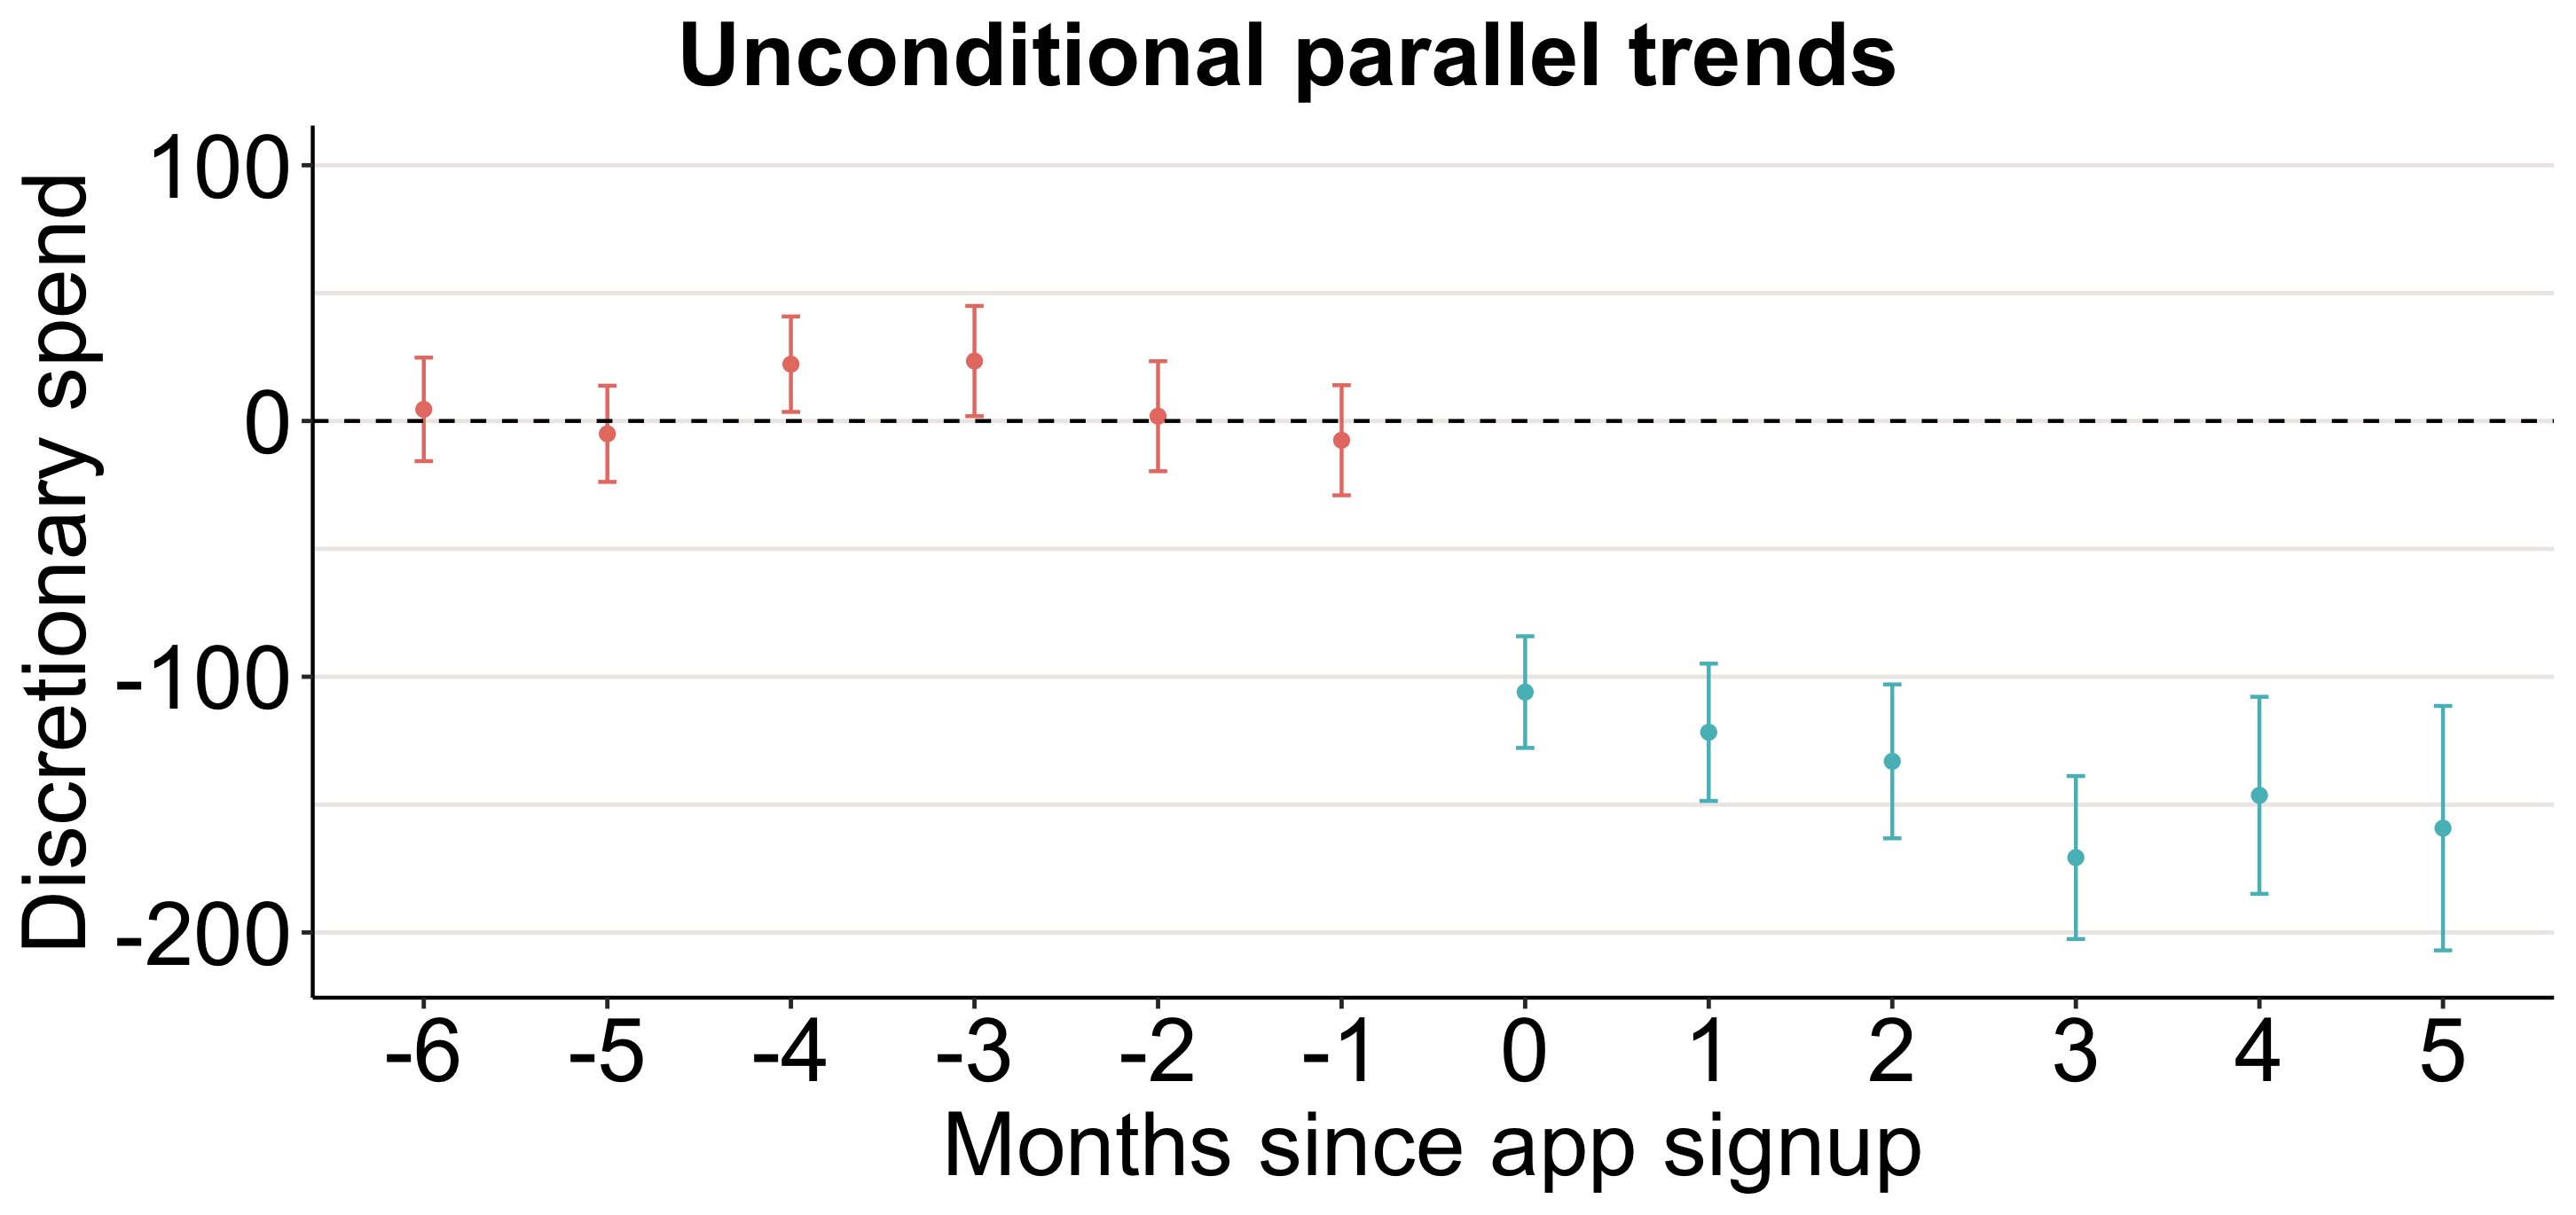
\includegraphics[width=.49\textwidth]{\figdir/dspend_uncond_es.png}
    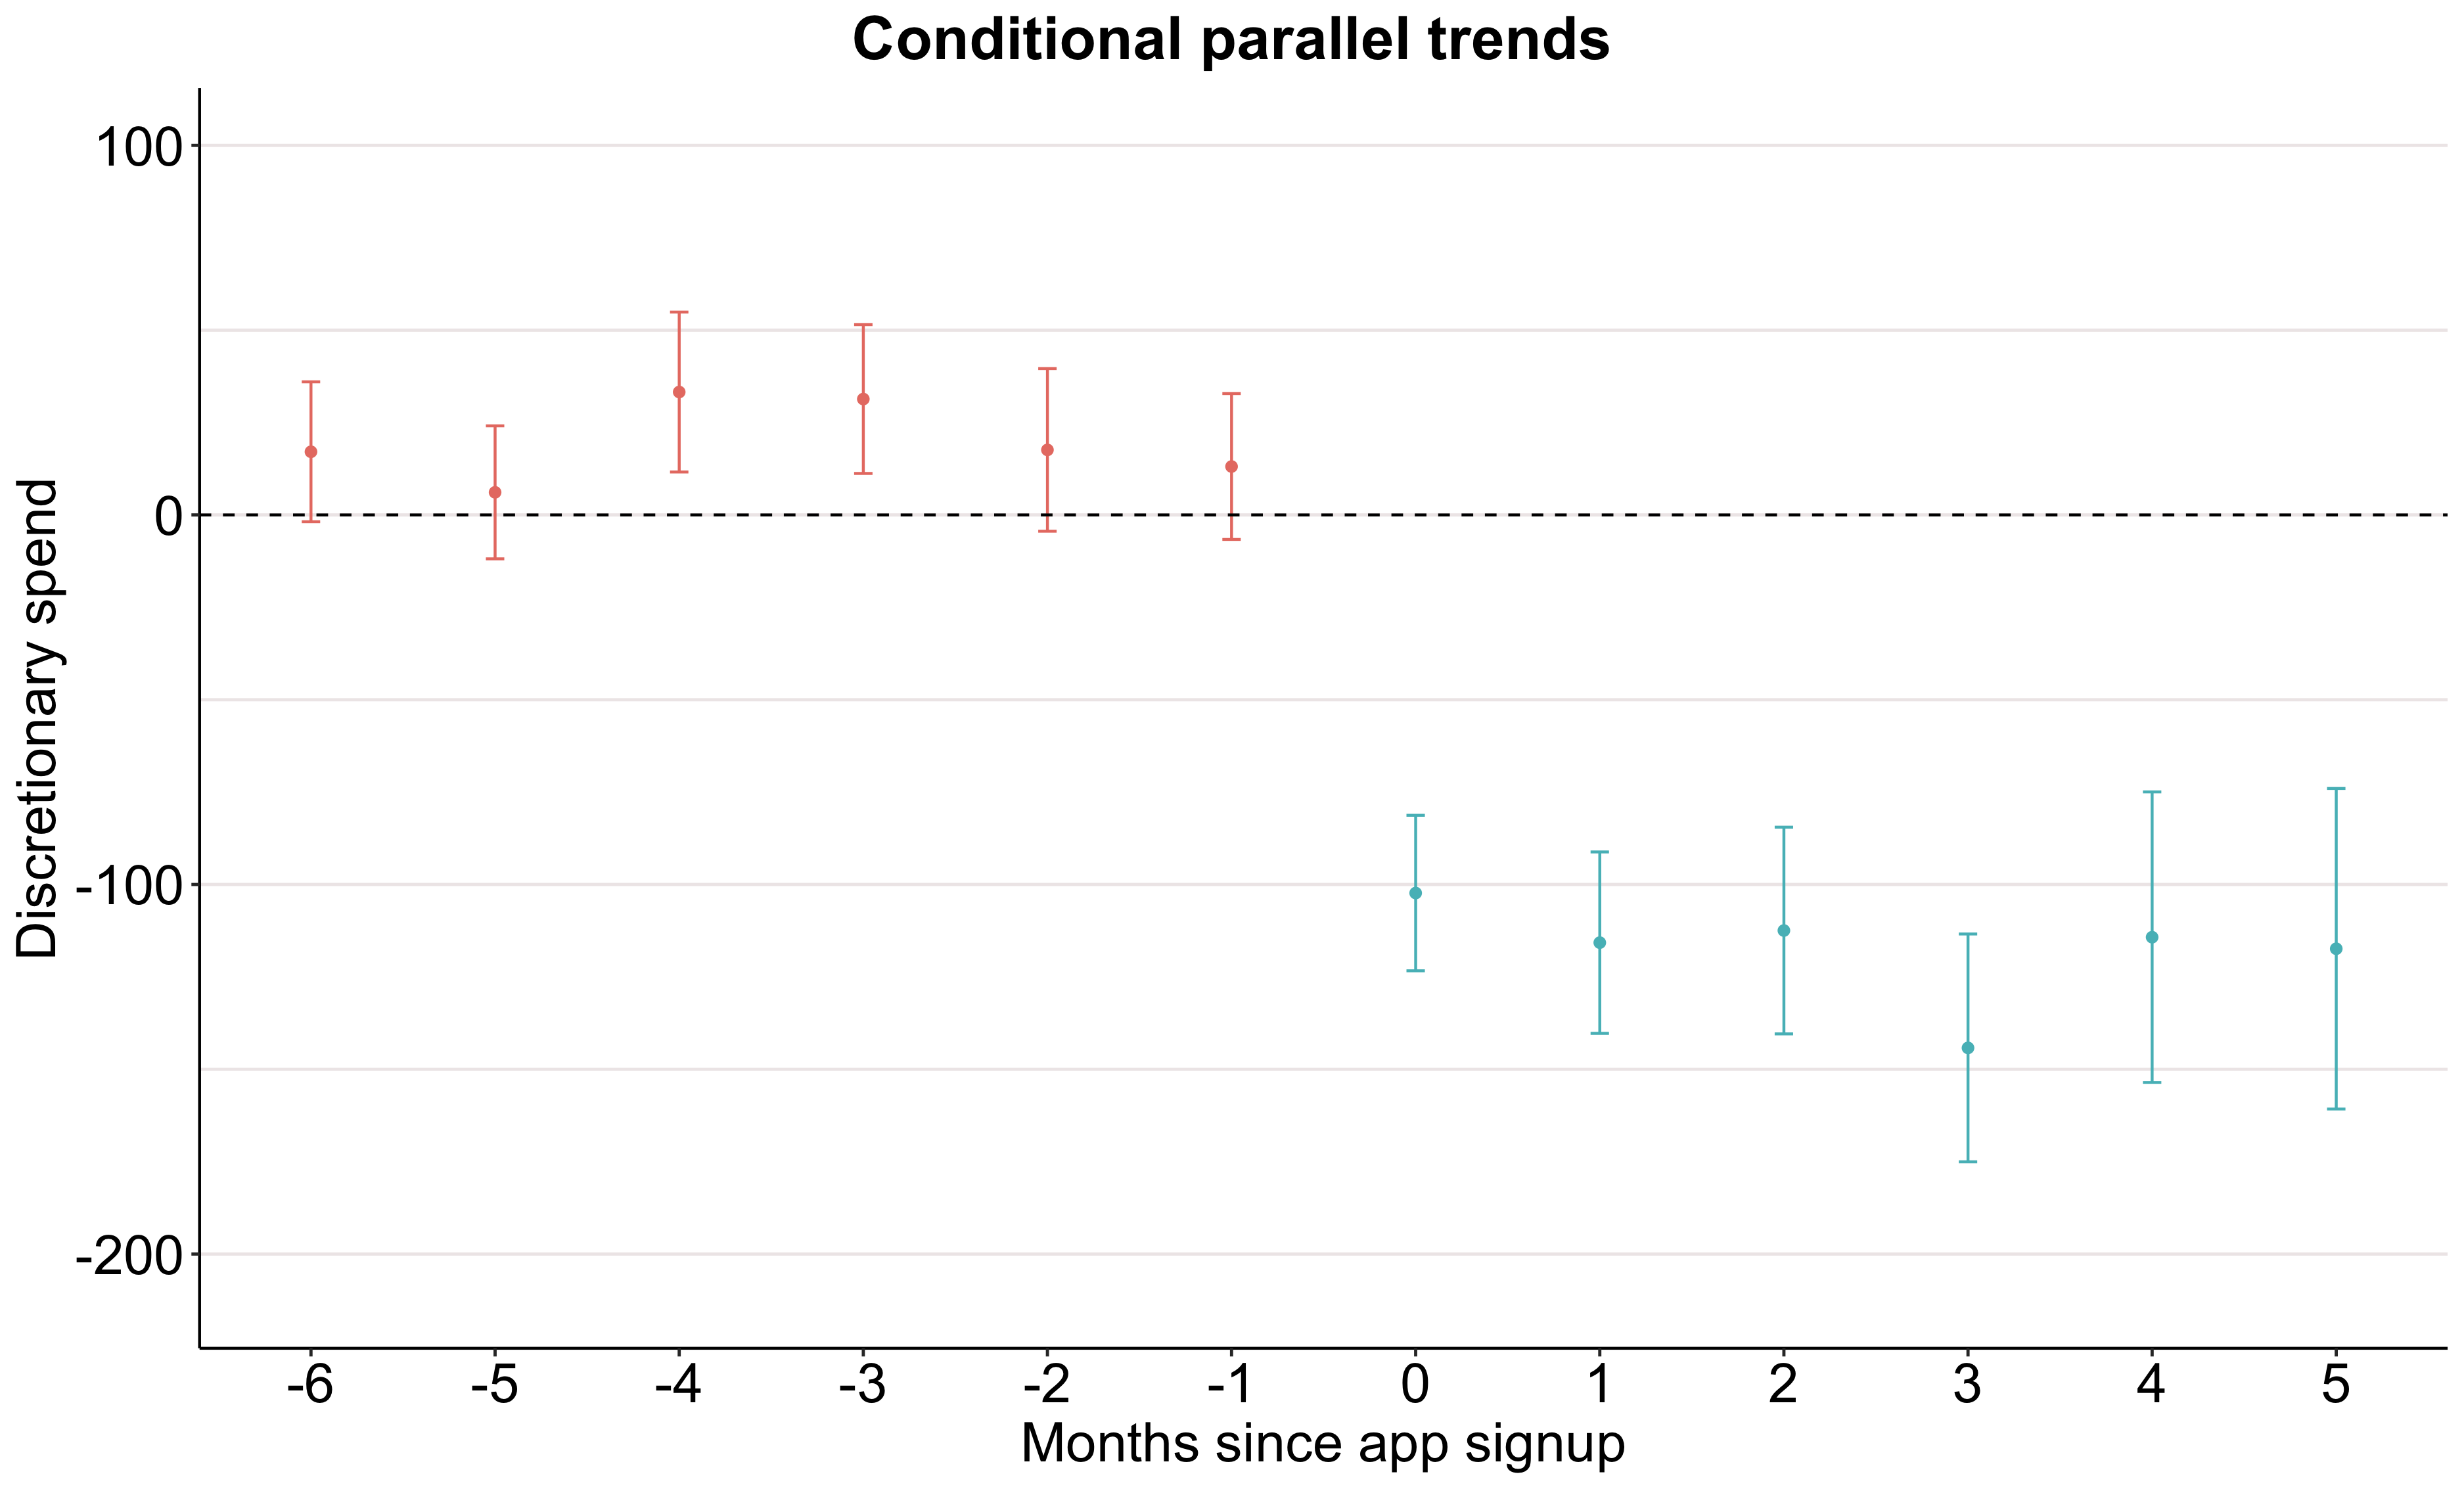
\includegraphics[width=.49\textwidth]{\figdir/dspend_cond_es.png}
    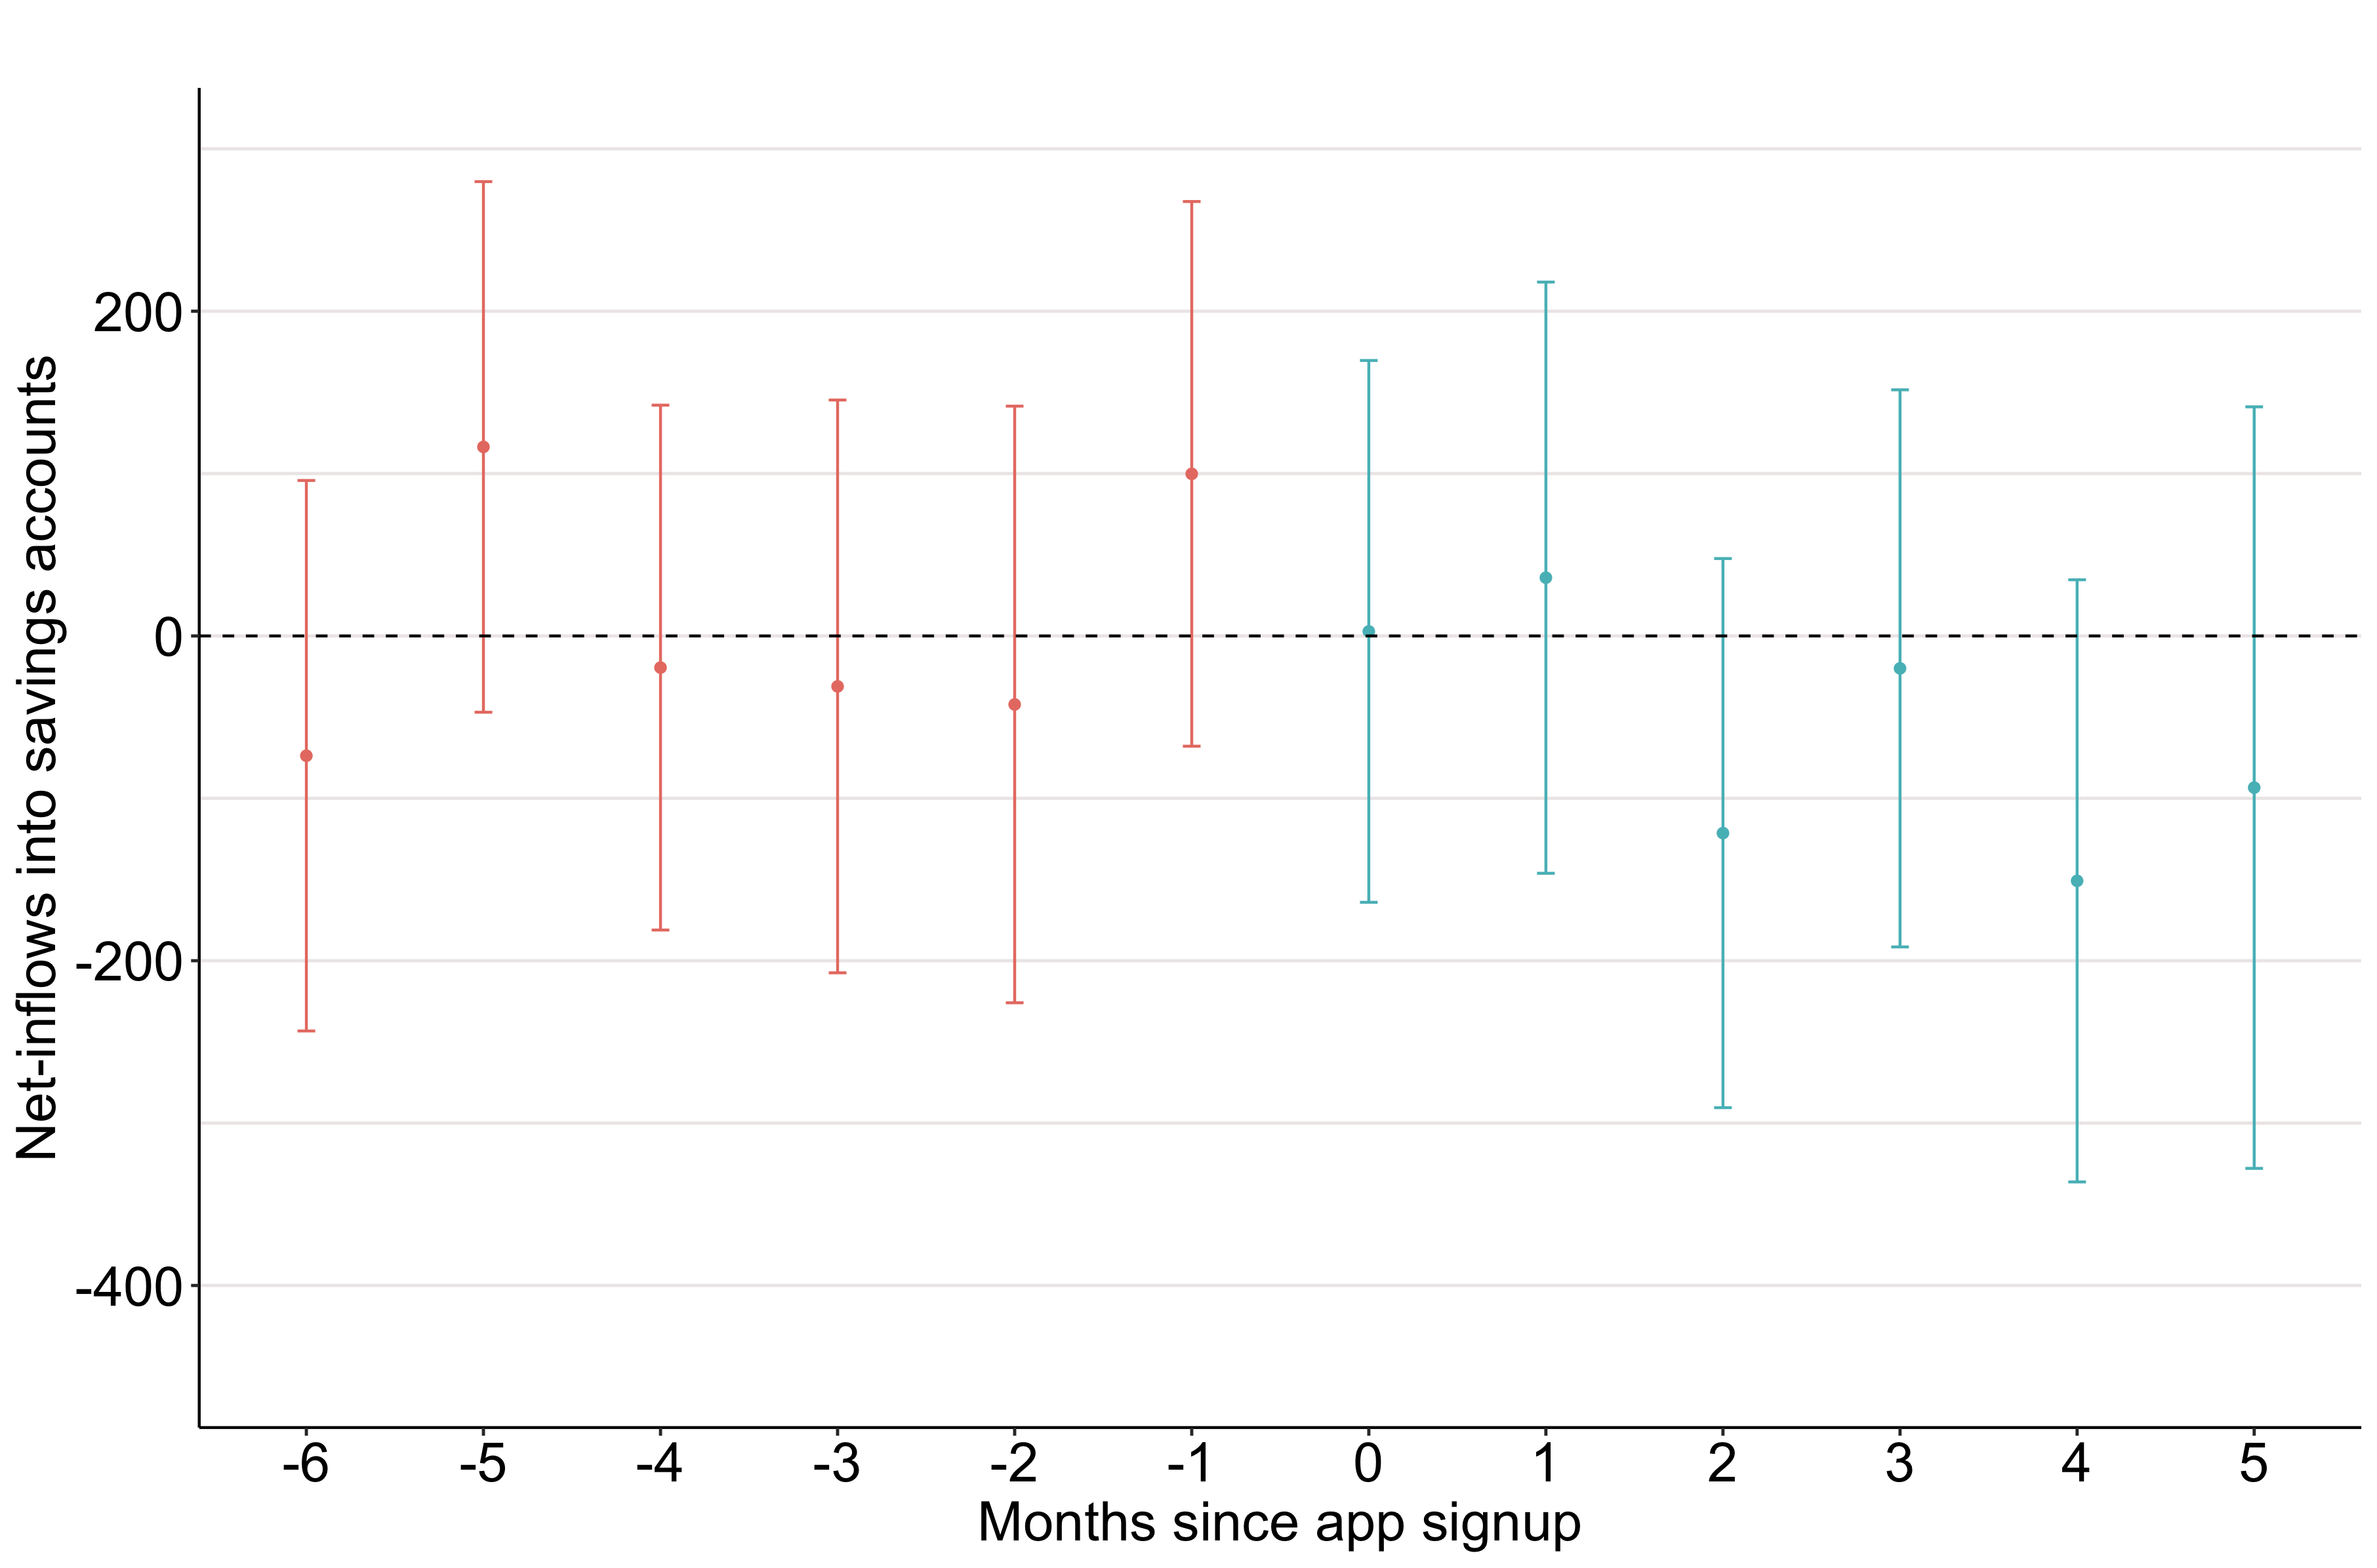
\includegraphics[width=.49\textwidth]{\figdir/netflows_uncond_es.png}
    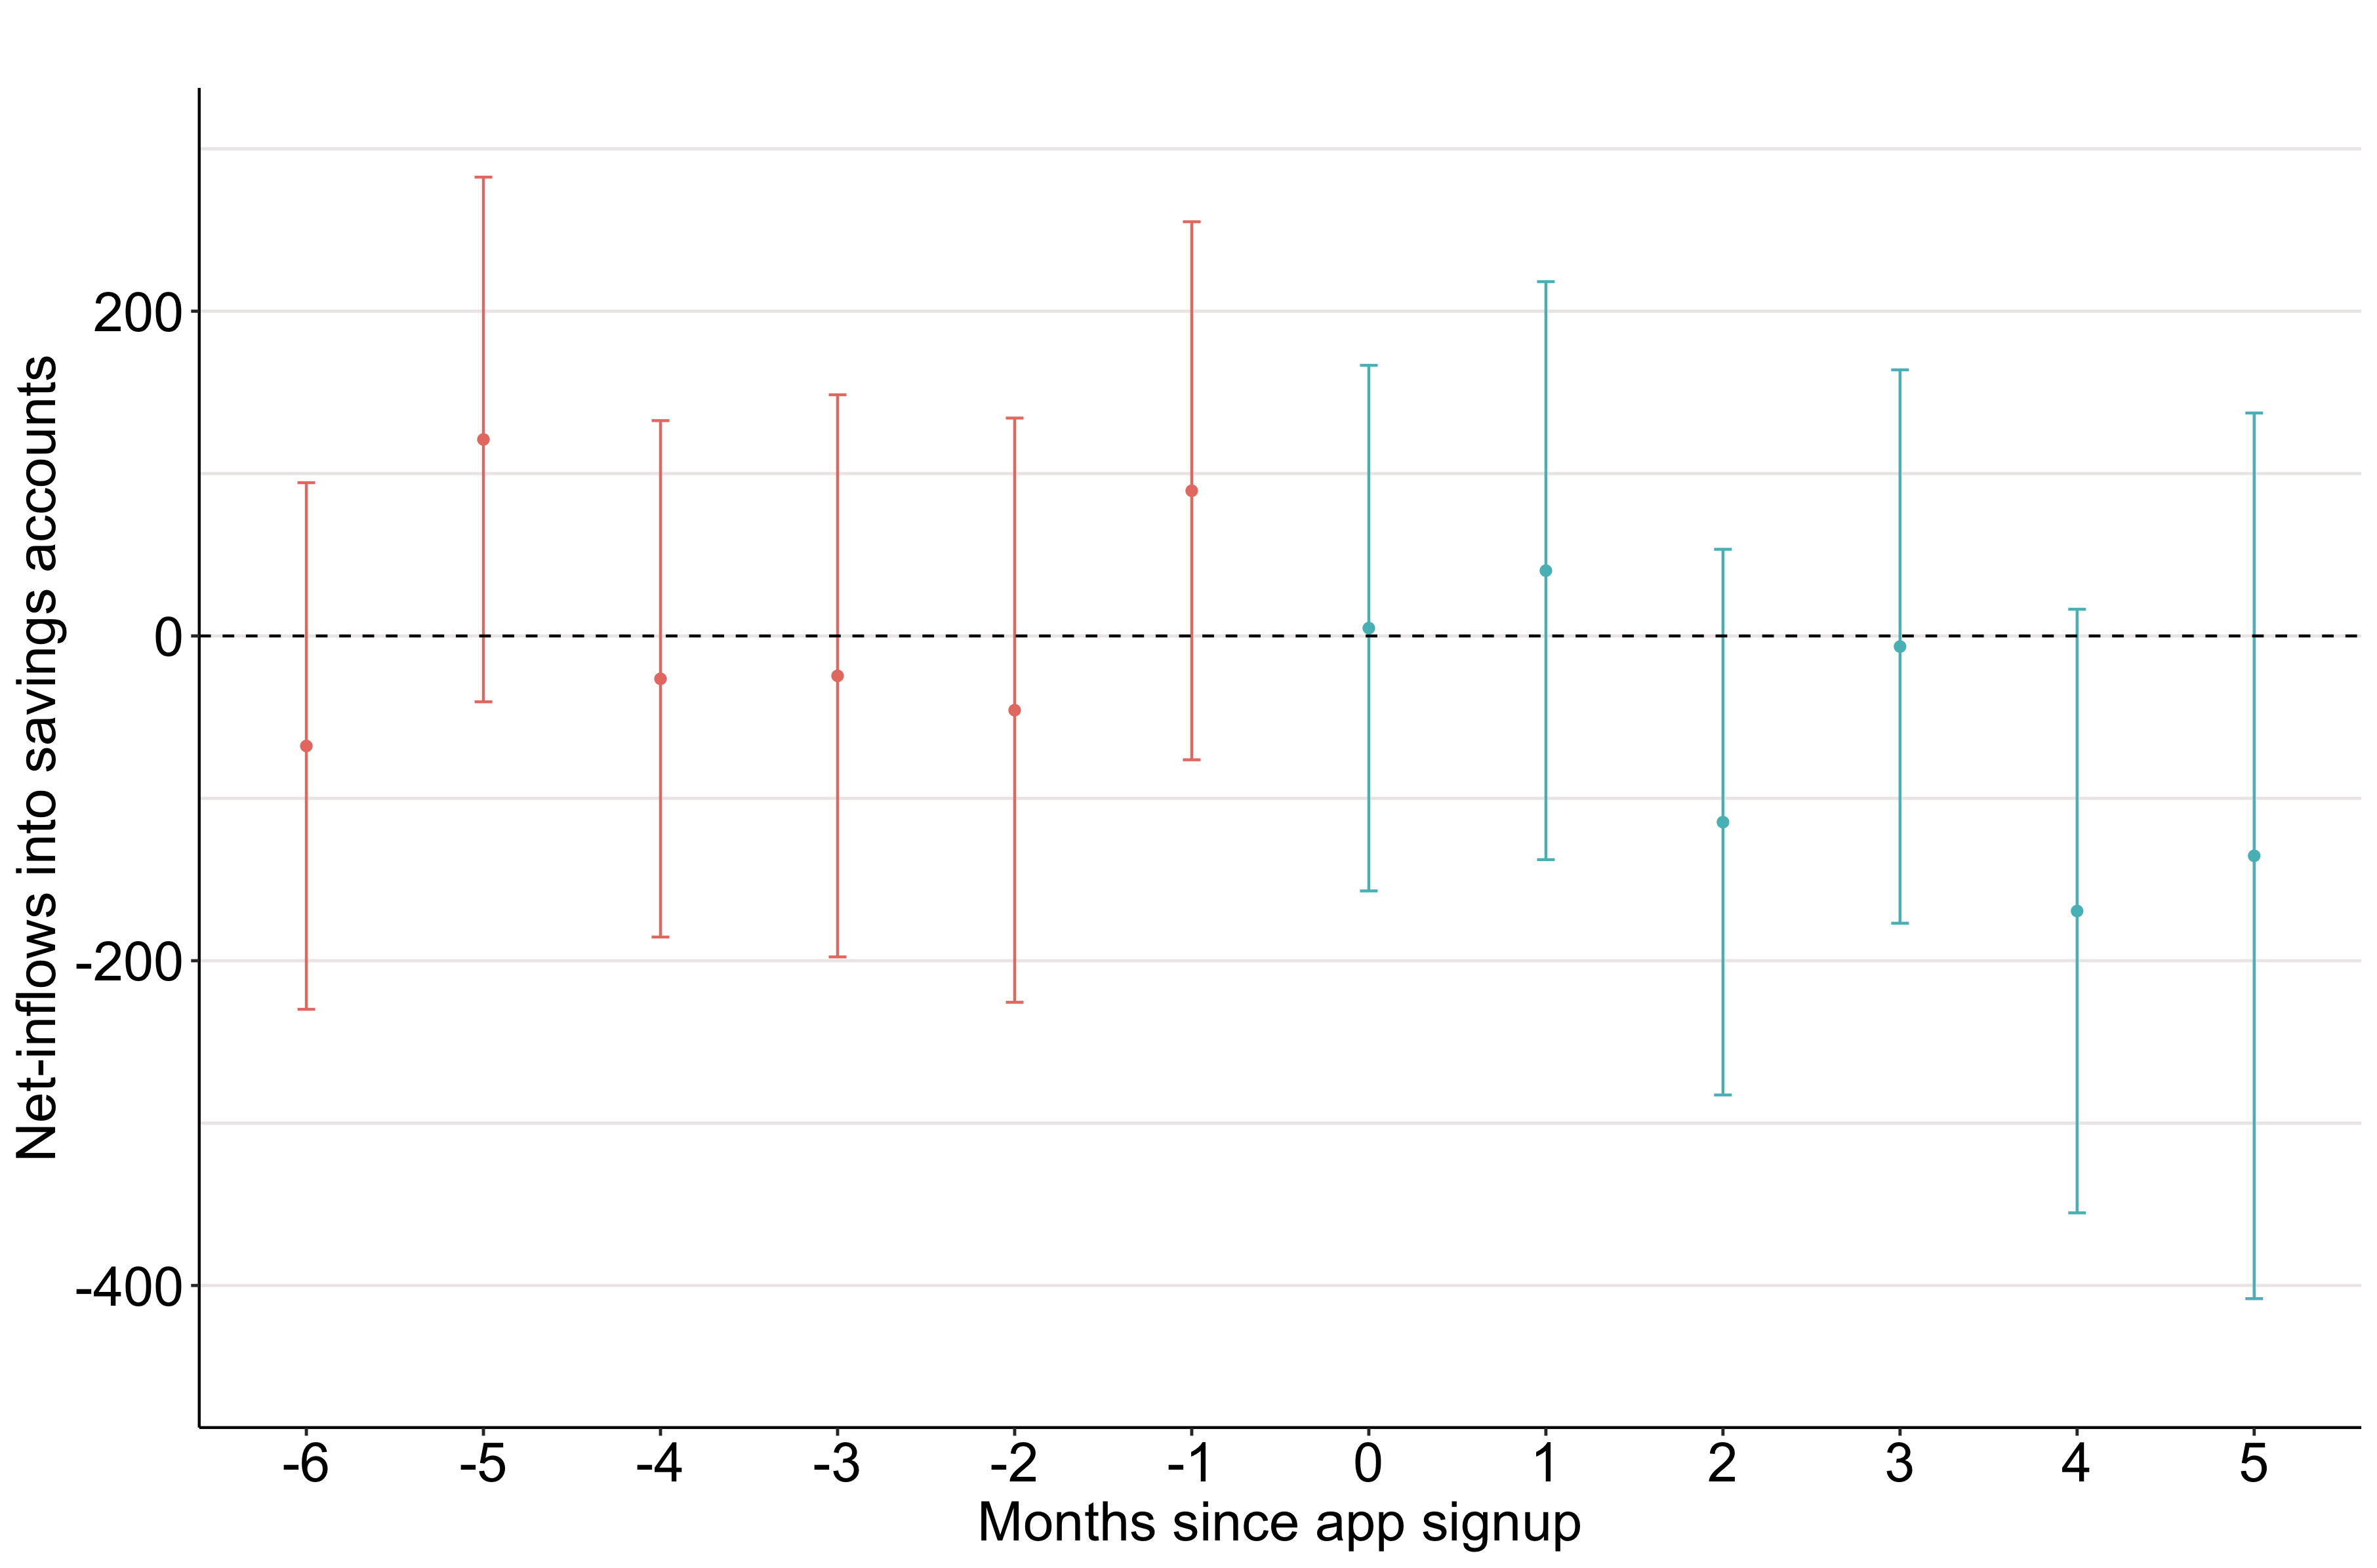
\includegraphics[width=.49\textwidth]{\figdir/netflows_cond_es.png}
    \fignote{\textwidth}{The effect of app use on monthly discretionary
        spending (top row) and monthly net-inflows into savings accounts
        (bottom row) under the unconditional (left column) and conditional
        (right column) parallel trends assumption. Point estimates represent
        group-time average treatment effects aggregated to periods since
        treatment exposure, as defined in Section~\ref{sub:estimation}. Red
        lines represent point estimates and uniform 95\% confidence bands for
        pre-treatment periods allowing for clustering at the user level. If the
        null hypothesis that parallel trends hold in all periods is correct,
        these should be equal to zero. Blue lines provide similar information
    for post-treatment periods.}
\end{figure}


\subsection{Intensive and extensive margins}%
\label{sub:intensive_and_extensive_margins}

\begin{itemize}

    \item Figure~\ref{fig:int_ext_results} shows the effect of app use on
        monthly discretionary spend (top row) and net-inflows into savings
        accounts (bottom row) disaggregated into the effect on the extensive
        (left column) and intensive (right column) margins. For discretionary
        spend, the extensive margin is the number of discretionary transactions
        per month, and the intensive margin is the average value of a
        discretionary spend transaction. For net-inflows into savings accounts,
        the extensive margin is the probability that net-inflows are positive
        in a given month, and the intensive margin is the value of net-inflows
        if net-inflows are positive.

    \item We can see that the reduction of discretionary spend seen in
        Figure~\ref{fig:main_results} is driven by changes on the extensive
        margin: users make about five fewer discretionary purchases once they
        start using the app, while the average amount of each purchase stays
        unchanged (and actually increases slightly over time). The mean value
        of a discretionary spend tranaction in our data is about \pounds25, so
        that five transactions account for the effect shown in the main
        results.

    \item As in the aggregated effects above, app use has no effect on savings
        behaviour.

\end{itemize}

\begin{figure}[H]
    \centering
    \caption{Intensive and extensive margins}%
    \label{fig:int_ext_results}
    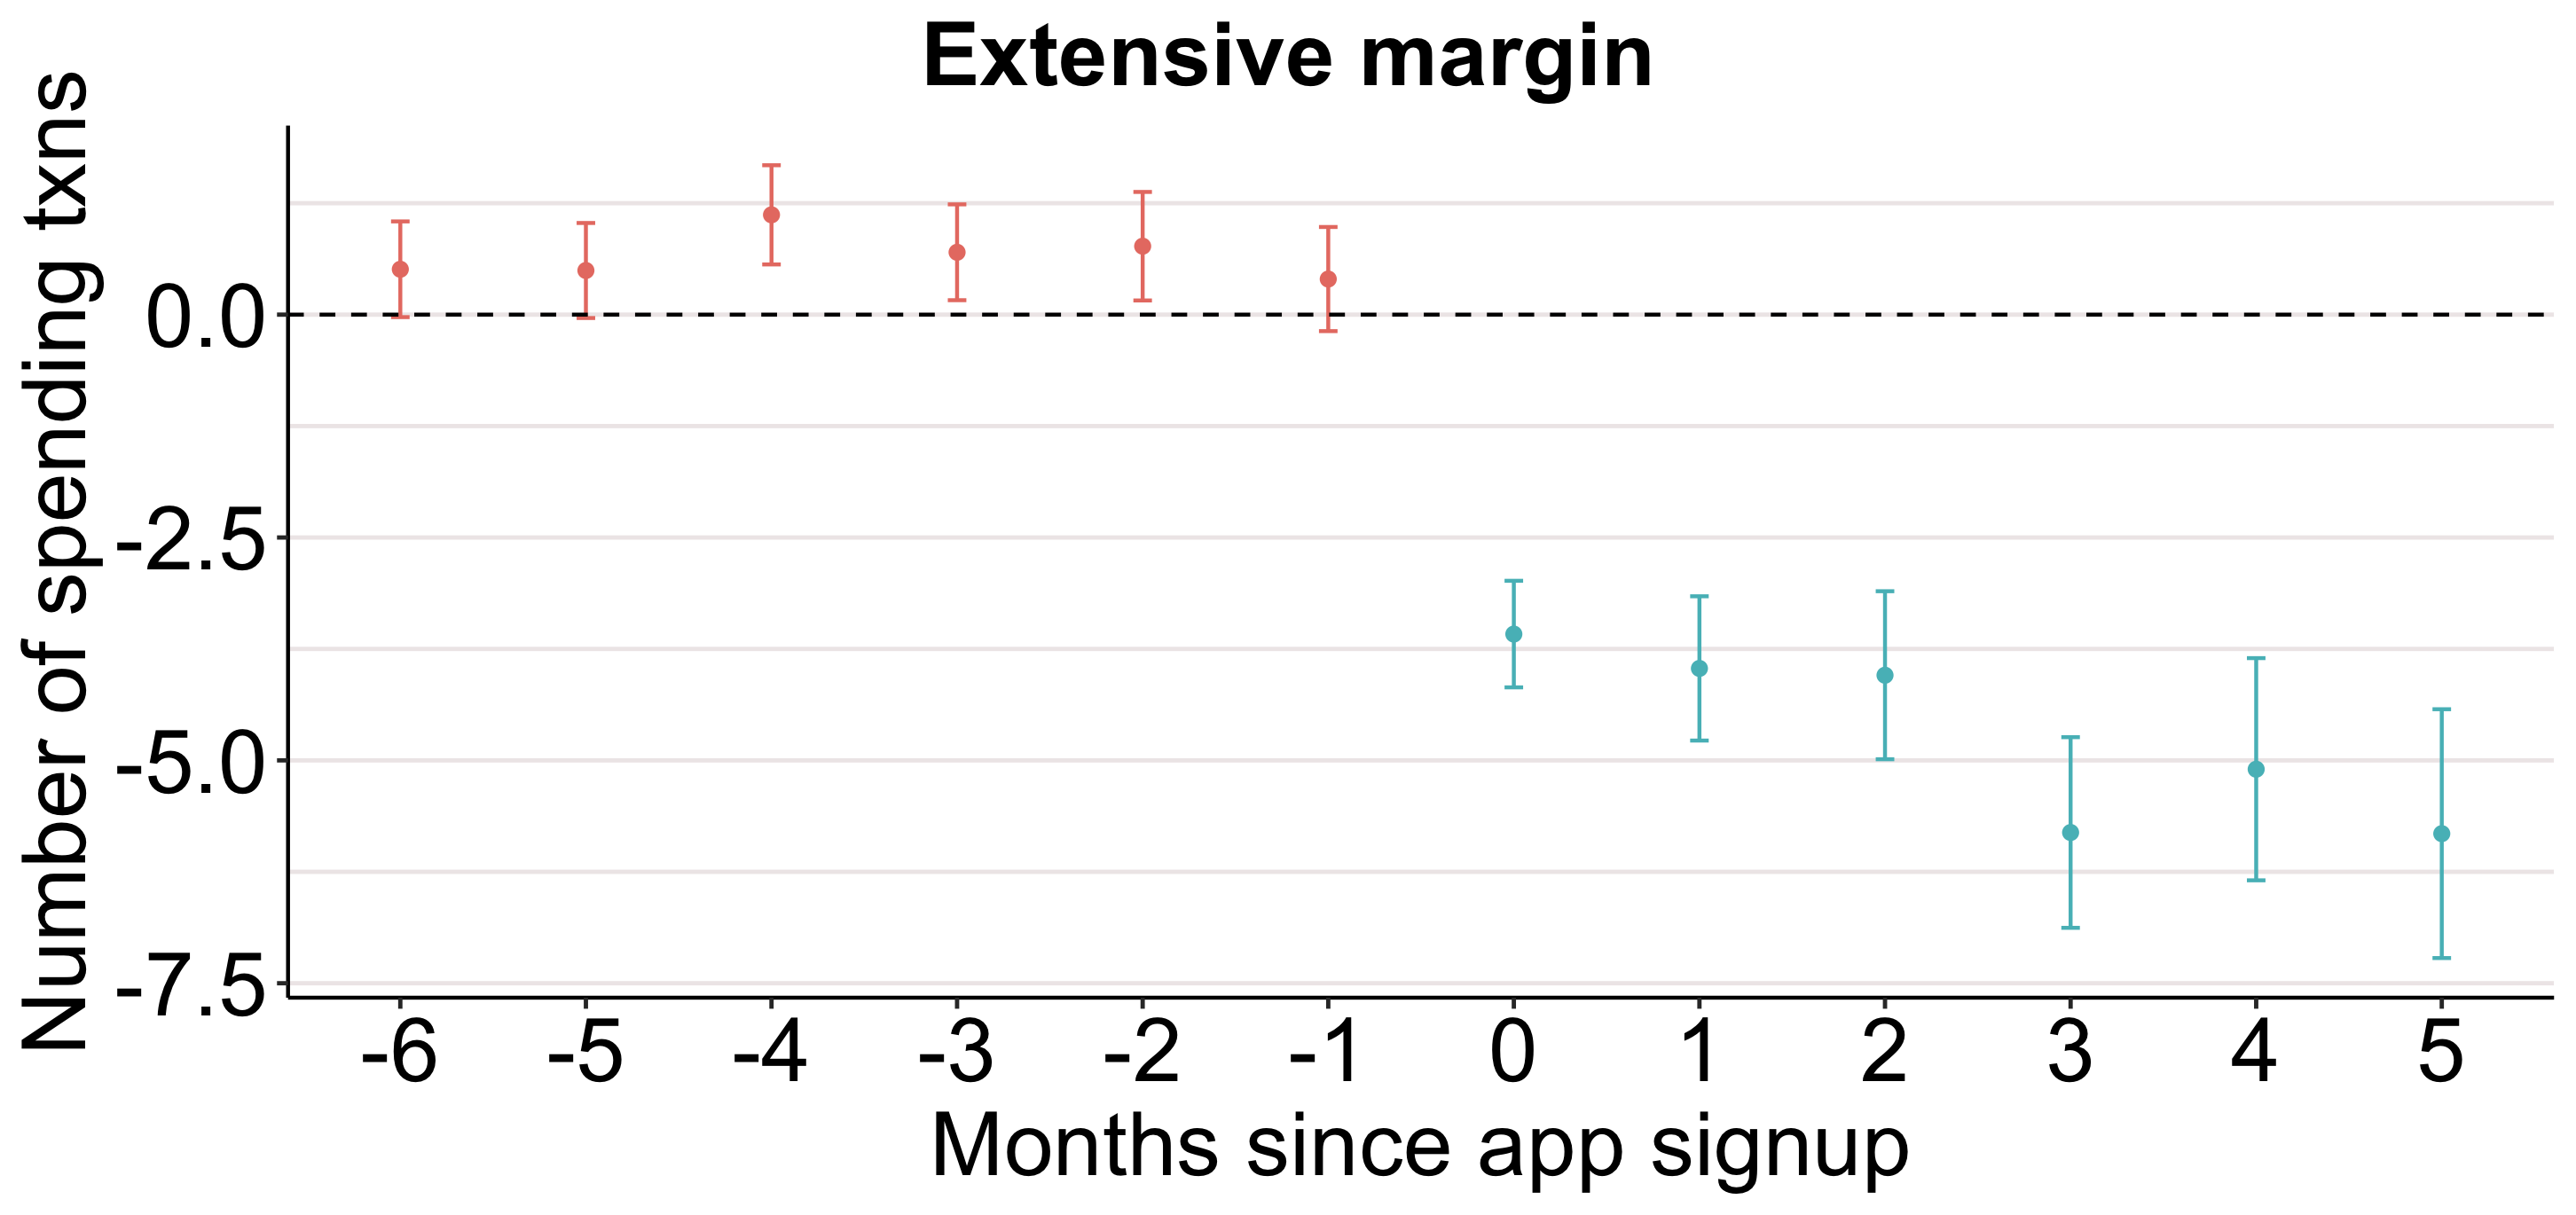
\includegraphics[width=.49\textwidth]{\figdir/dspend_extens_es.png}
    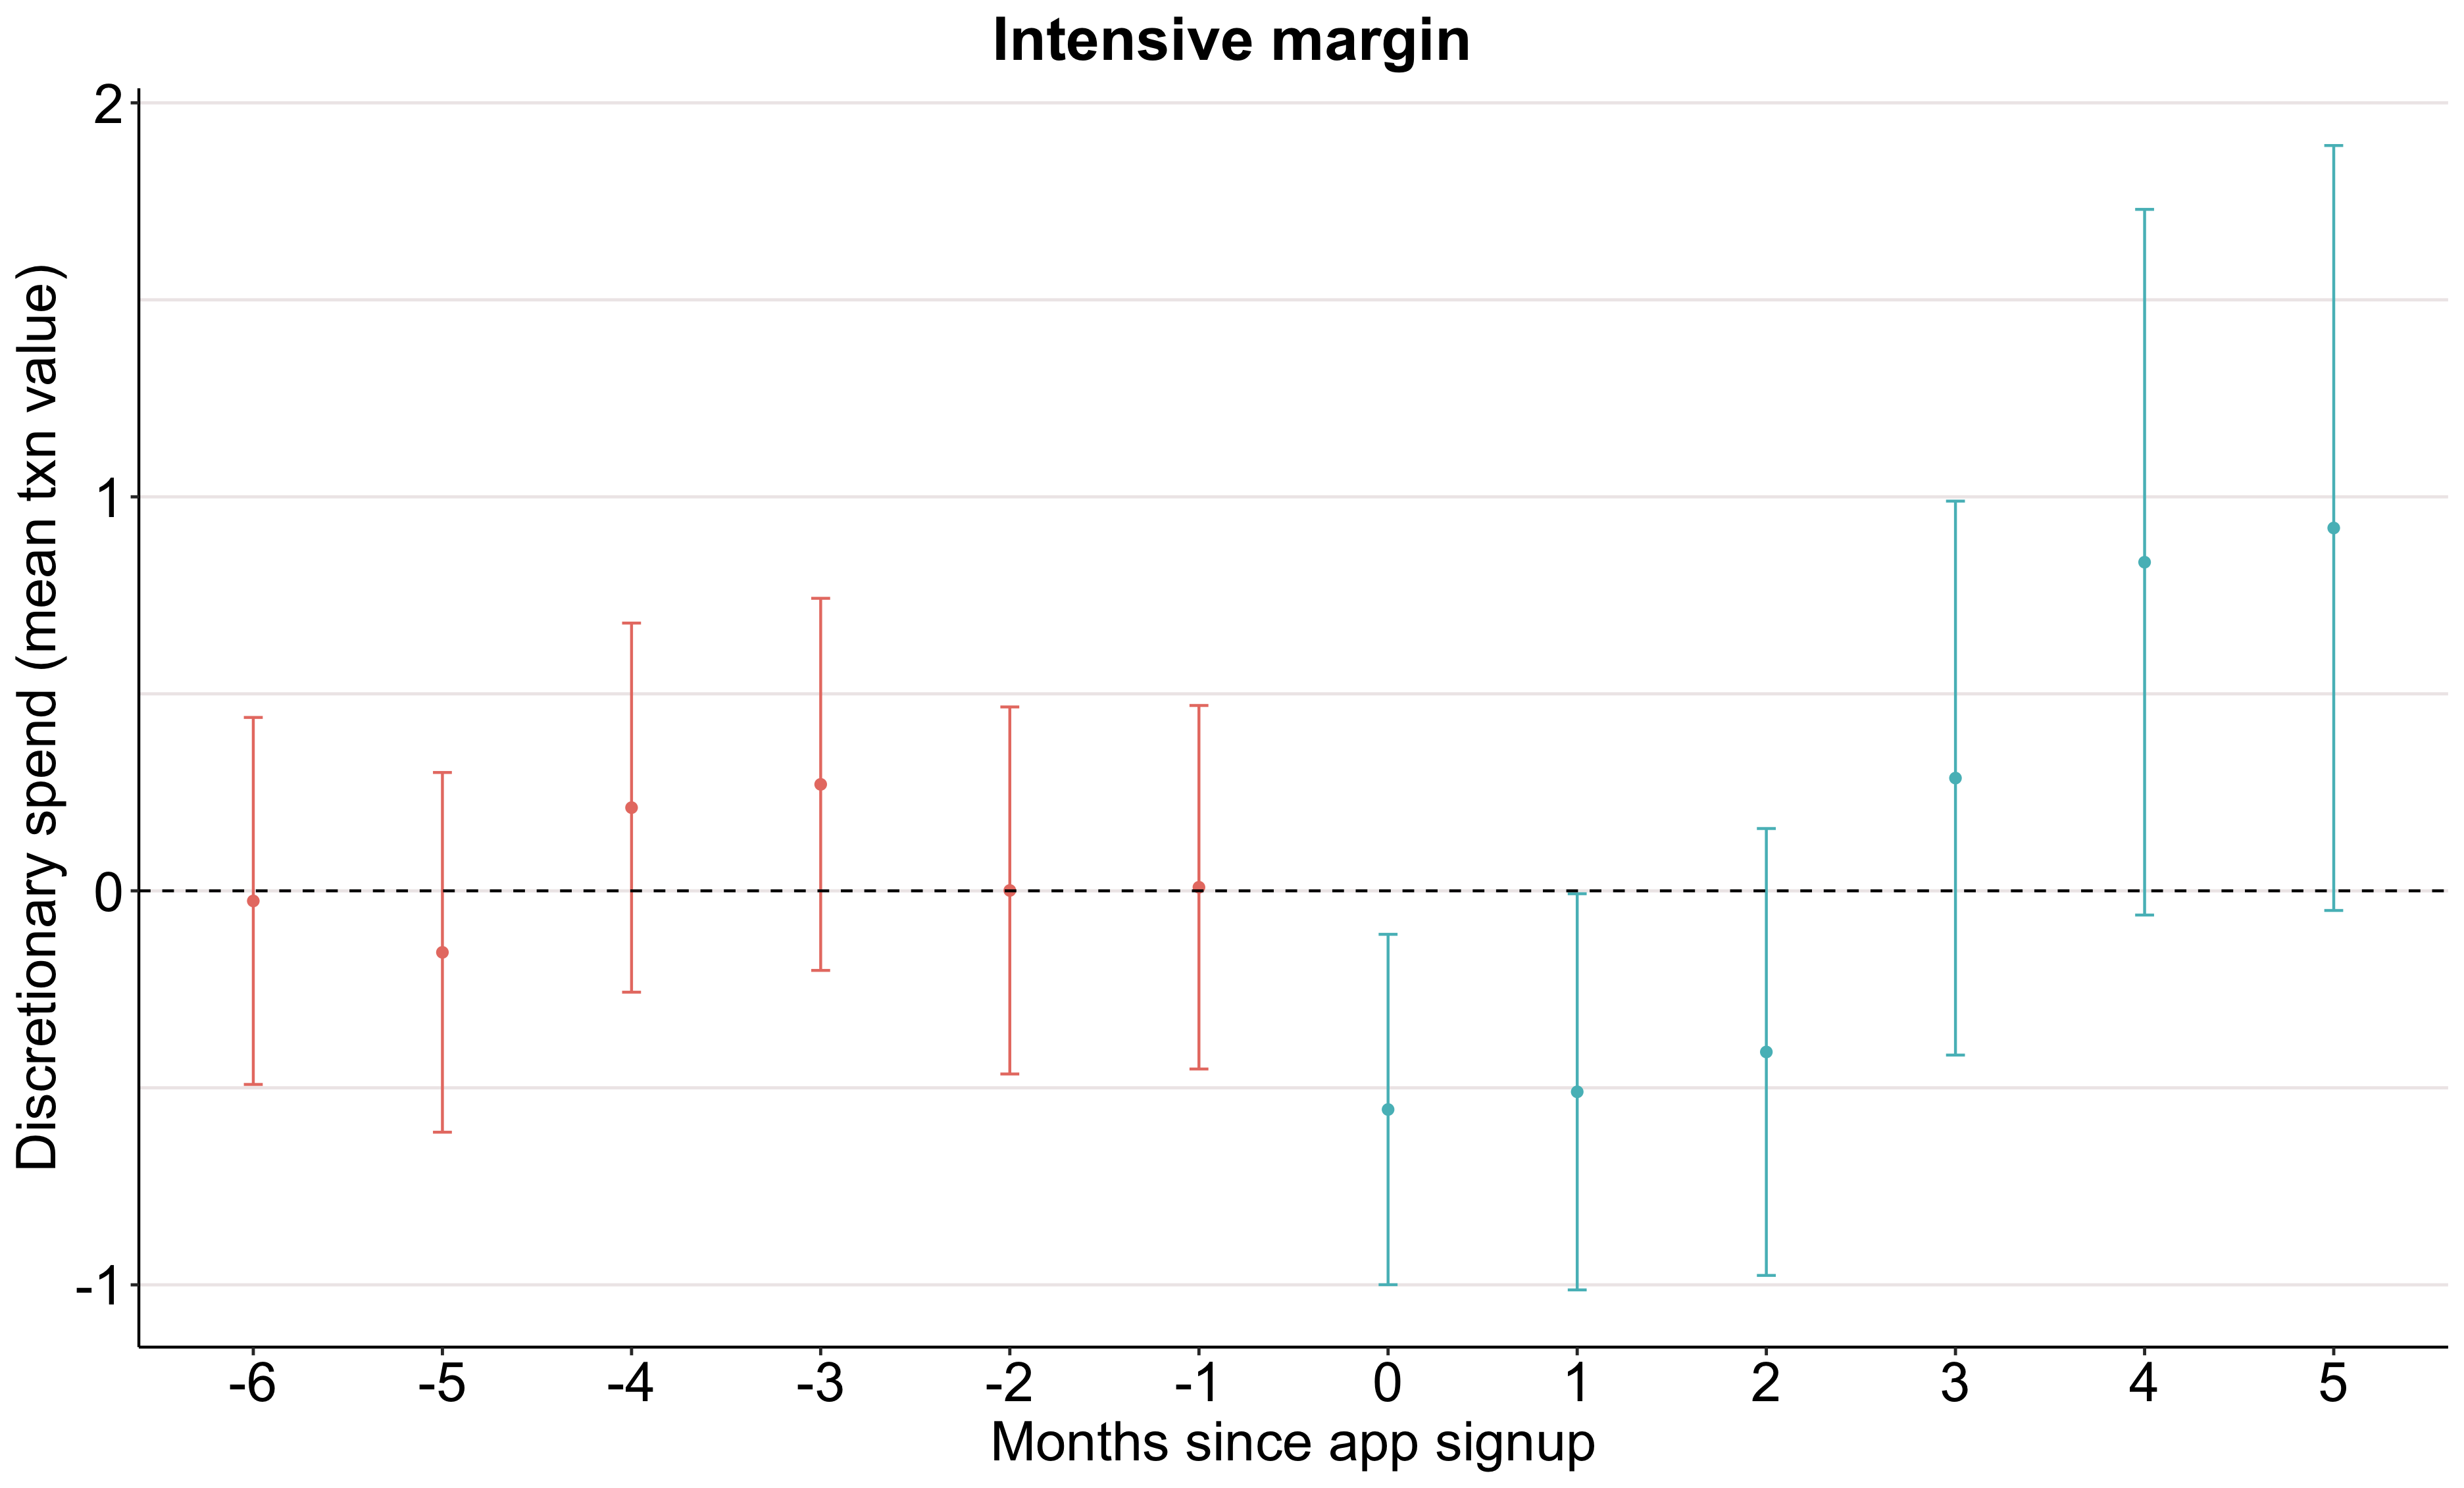
\includegraphics[width=.49\textwidth]{\figdir/dspend_intens_es.png}
    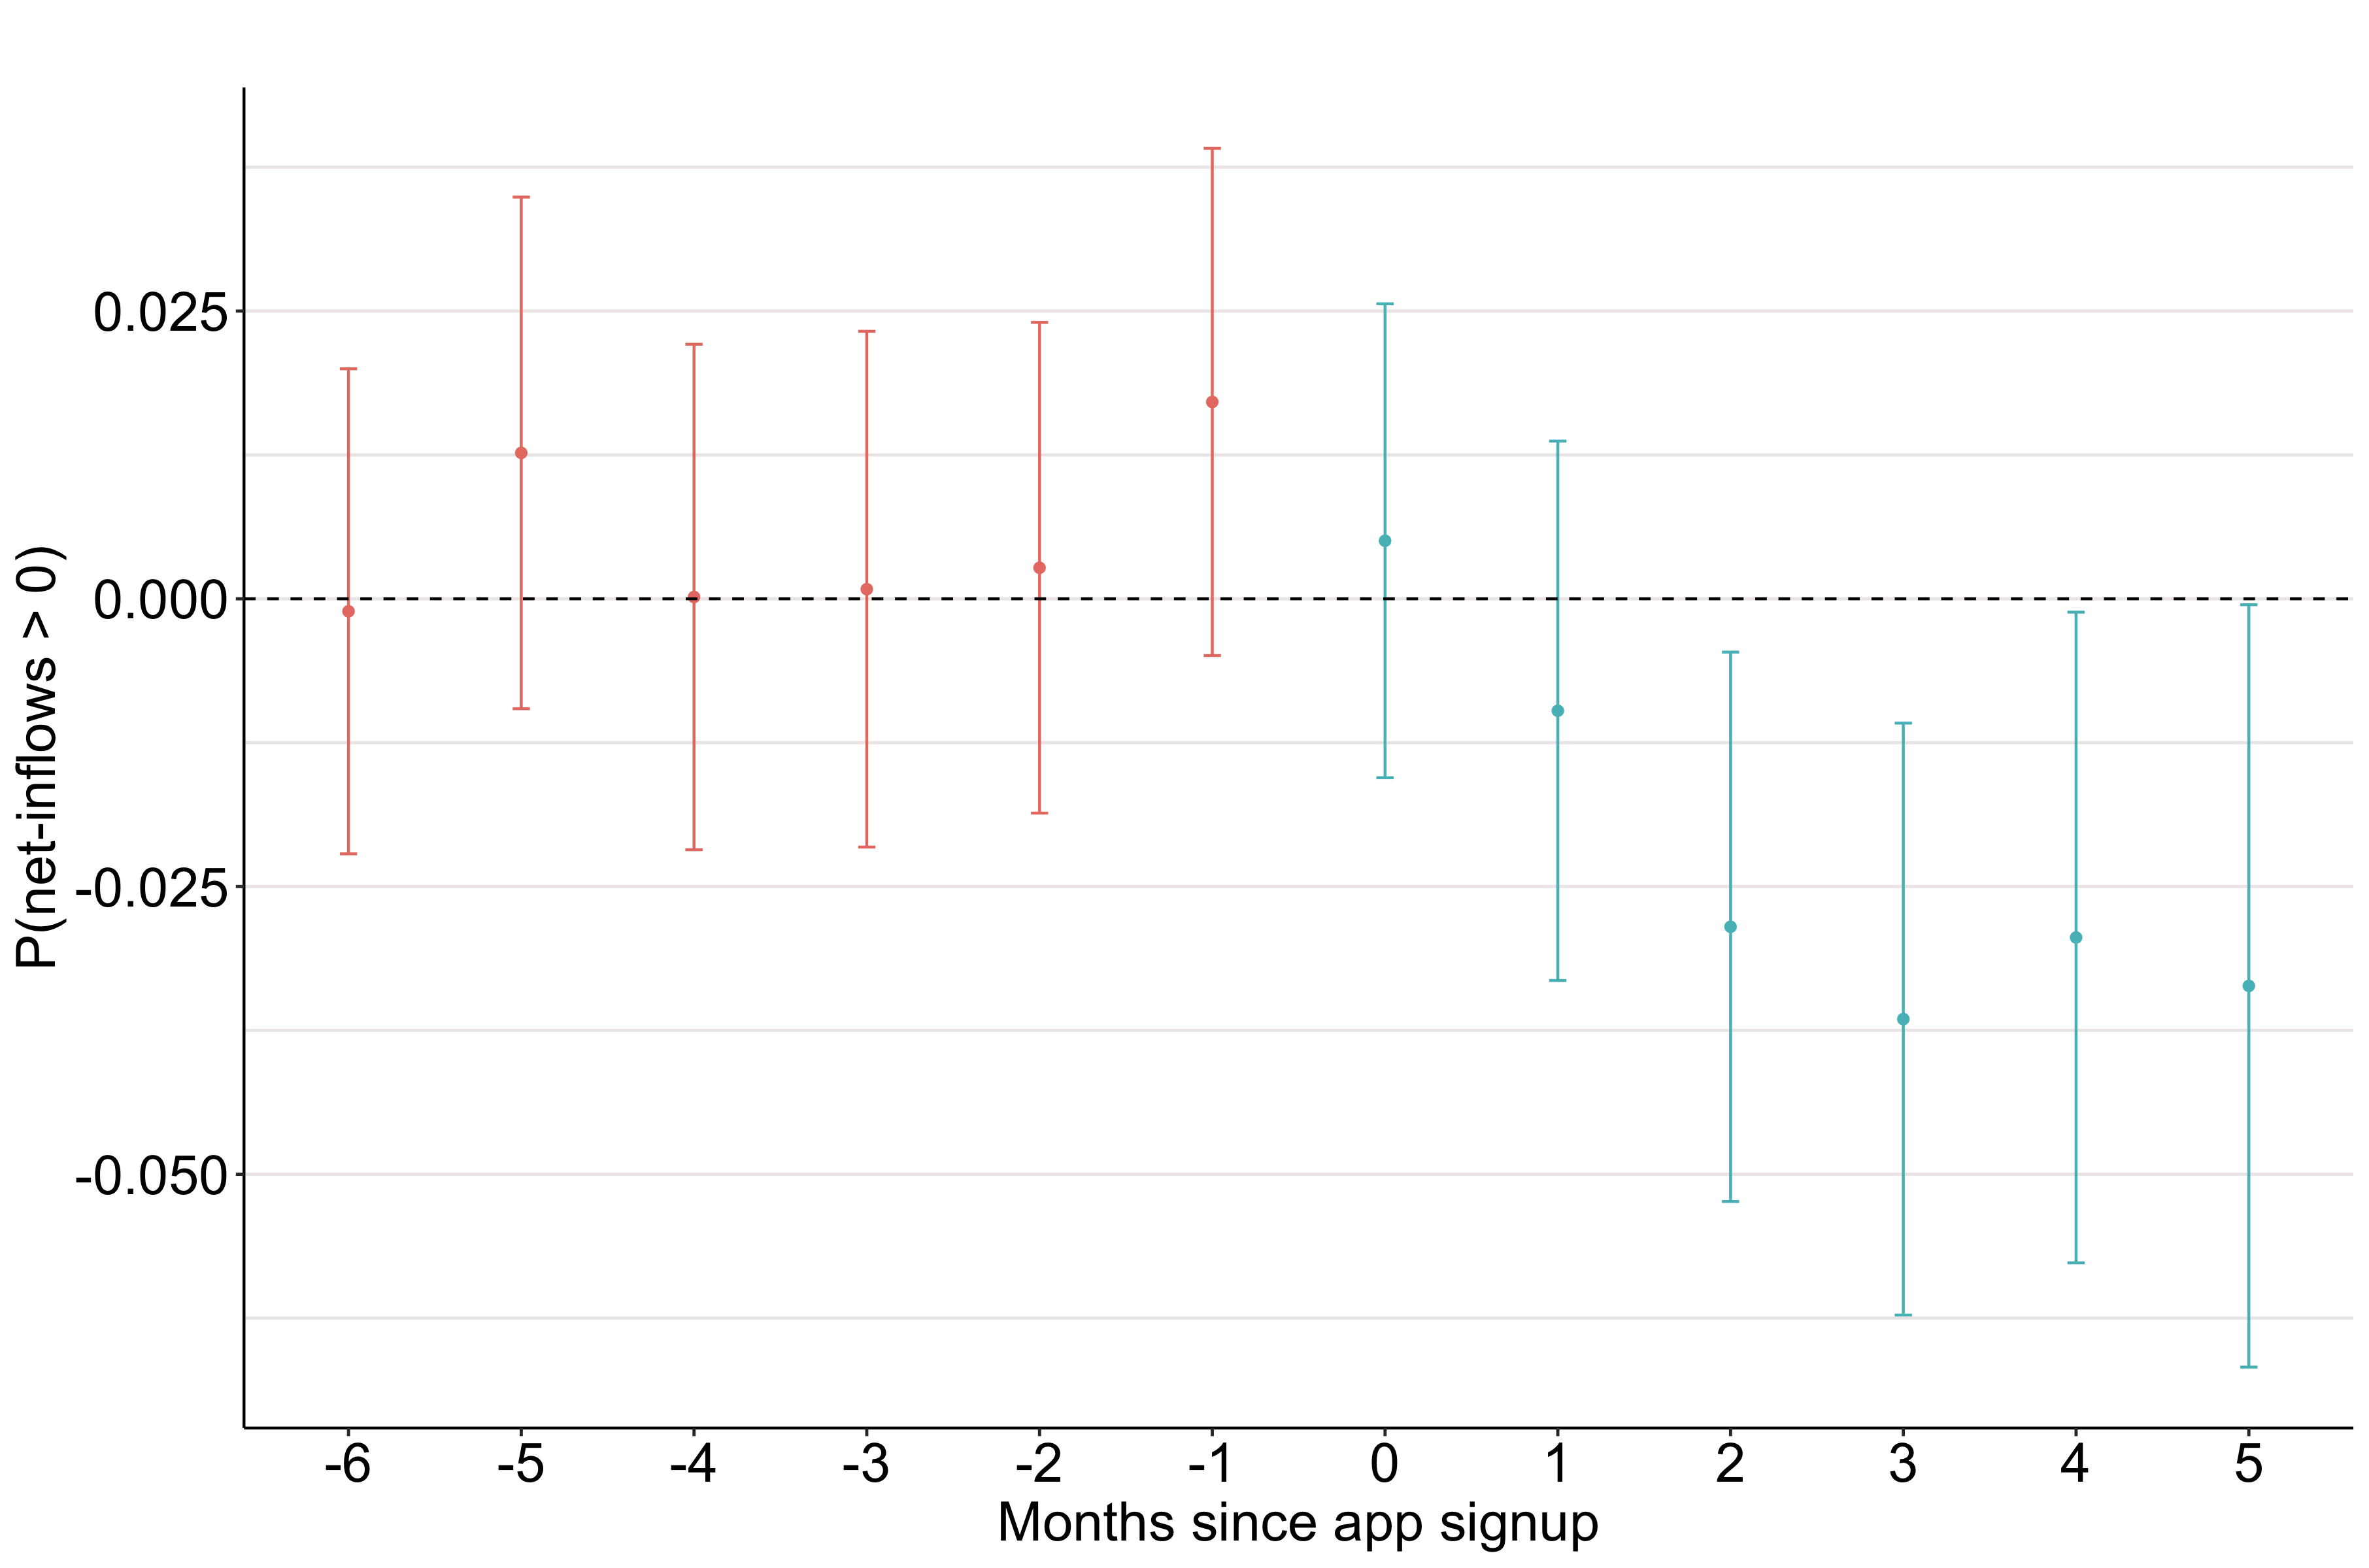
\includegraphics[width=.49\textwidth]{\figdir/netflows_extens_es.png}
    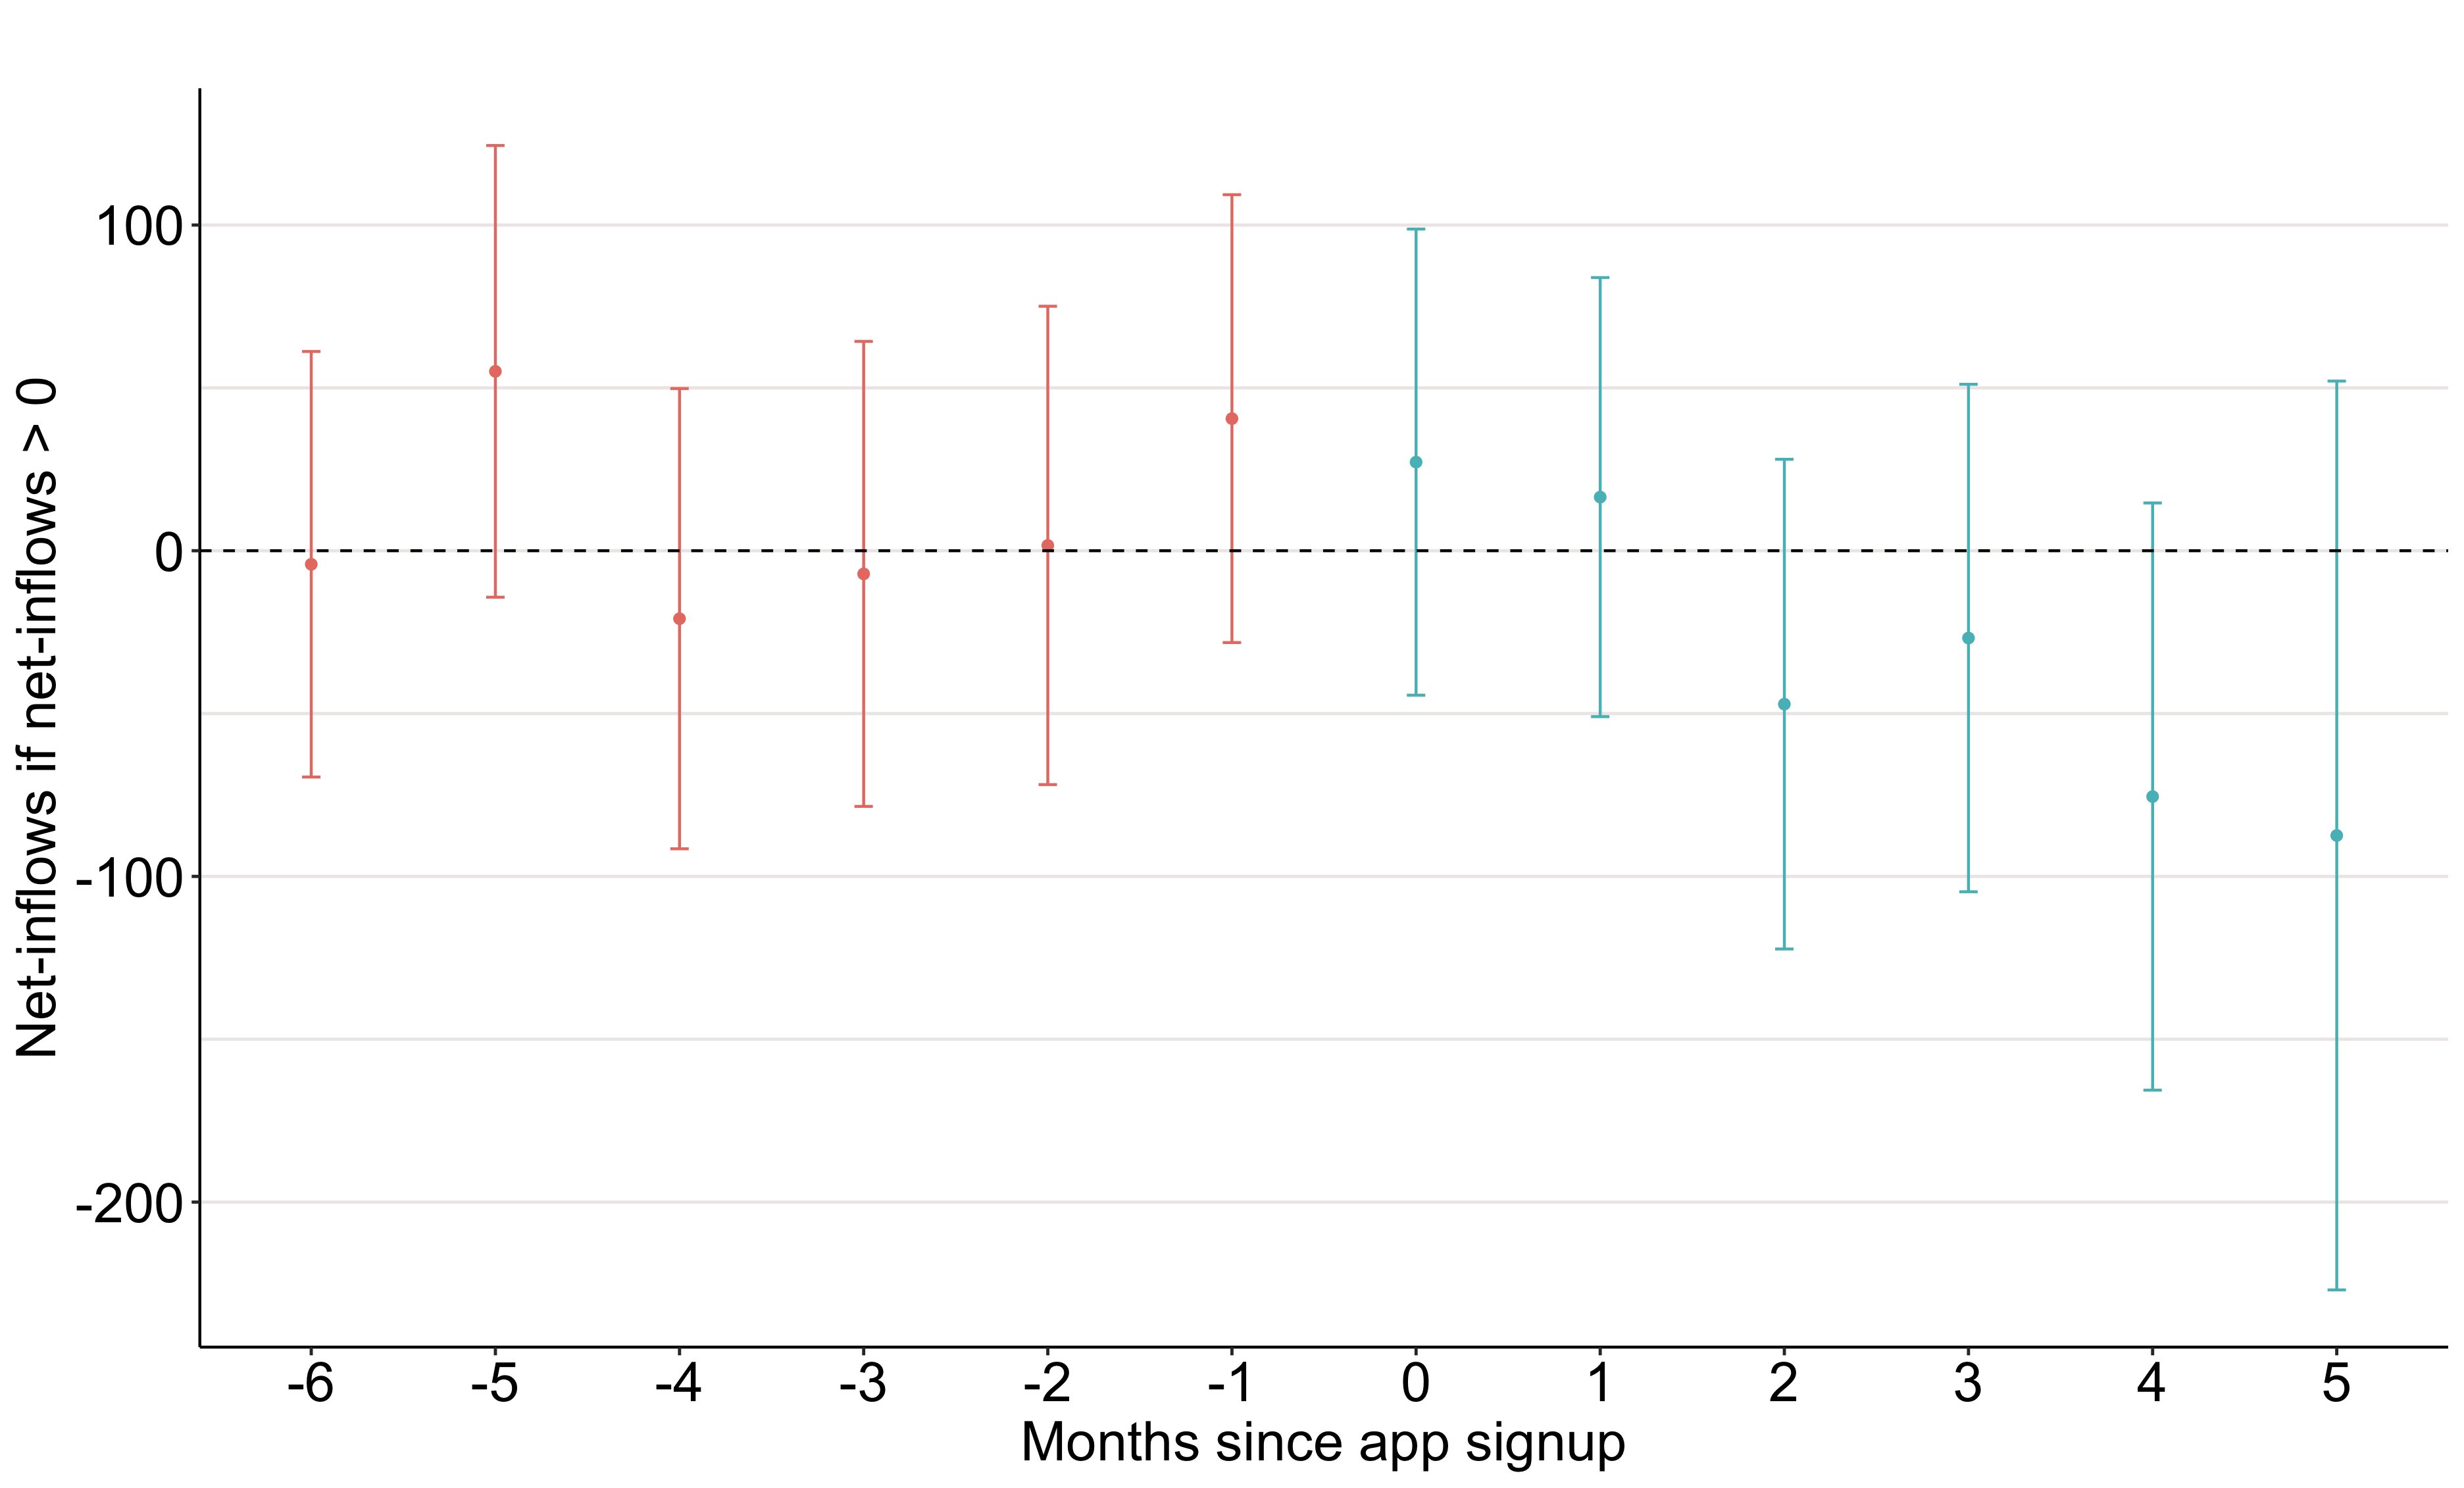
\includegraphics[width=.49\textwidth]{\figdir/netflows_intens_es.png}
    \fignote{\textwidth}{The effect of app use on monthly discretionary spend
        (top row) and net-inflows into savings accounts (bottom row)
        disaggregated into the effect on the extensive (left column) and
        intensive (right column) margins. For discretionary spend, the
        extensive margin is the number of discretionary transactions per month,
        and the intensive margin is the average value of a discretionary spend
        transaction. For net-inflows into savings accounts, the extensive
        margin is the probability that net-inflows are positive in a given
        month, and the intensive margin is the value of net-inflows if
        net-inflows are positive. Point estimates represent
        group-time average treatment effects aggregated to periods since
        treatment exposure, as defined in Section~\ref{sub:estimation}. Red
        lines represent point estimates and uniform 95\% confidence bands for
        pre-treatment periods allowing for clustering at the user level. If the
        null hypothesis that parallel trends hold in all periods is correct,
        these should be equal to zero. Blue lines provide similar information
    for post-treatment periods.}
\end{figure}


\subsection{Where do additional funds go?}%
\label{sub:where_do_additional_funds_go_}

\begin{itemize}
    \item Above we find that app use reduces discretionary spend but does not
        increase flows into savings accounts.

    \item This begs the question: ``Where does the money go?``

    \item One possibility is that people do save more but that the additional
        savings go into either long-term investment accounts that cannot be
        linked to the app (e.g. accounts at Vanguard or other investment
        services) or into conventional savings accounts that people users do
        not link to the app. Check for additional outgoing transfers to
        investment services and transfers into accounts that are not added to
        app.

    \item I first look at flows into investment accounts.

    \item Then at transfers from current accounts. Here I consider two metrics.
        First, savings defined by users, second, total transfers.

    \item Another possibility is that people pay down debt. Can check whether
        payments into credit card accounts or repayment of loands increases.

    \item Here, I first look at flows into credit card accounts.

    \item Then at loan repayments. Control for loan takeout. Actually, plot
        separately, then control for takeout in repayment in case there is a
        pattern.

    \item Credit card payment pattern can be explained by people making fewer
        credit card purchases and hence making fewer payments (dspend includes
        credit card purchases).

    \item Insignificant results suggest that additional savings dissipate
        across multiple streams, either across people (some people save, some
        pay down debt, etc.) or even within each person.

\end{itemize}

\begin{figure}[H]
    \centering
    \caption{Possible destinations of reduced spend funds}%
    \label{fig:int_ext_results}
    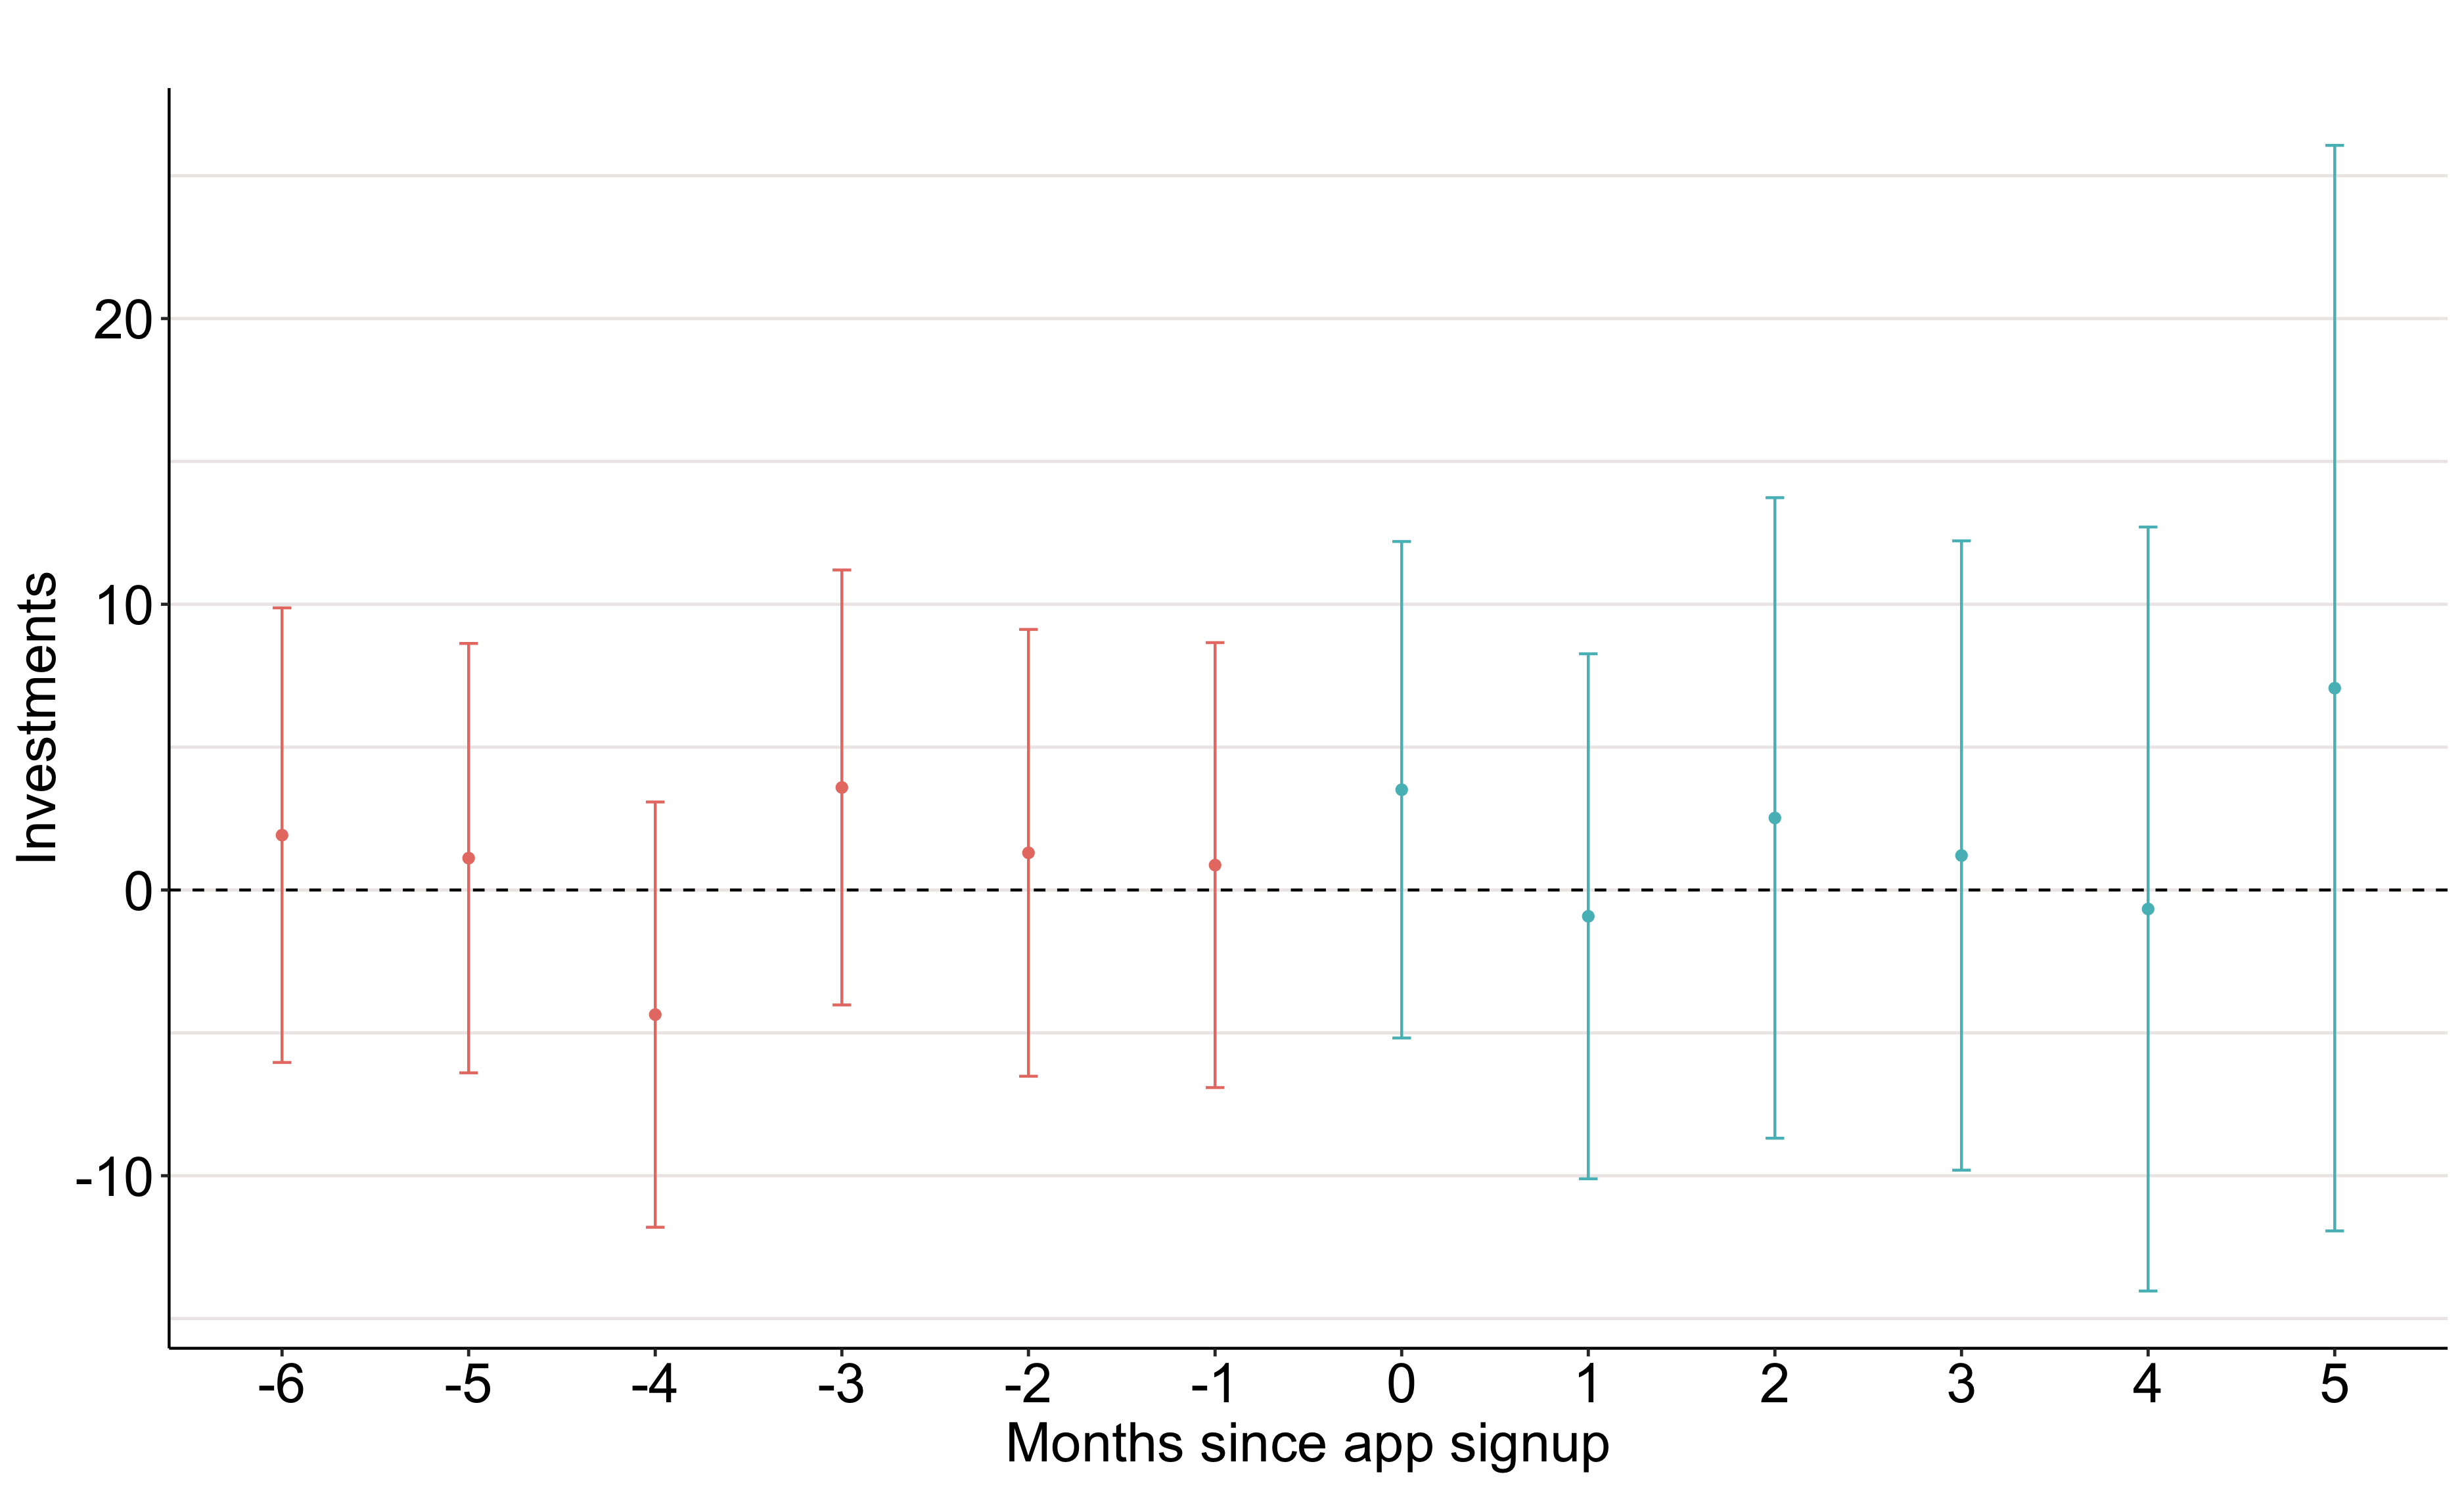
\includegraphics[width=.49\textwidth]{\figdir/investments_cond_es.png}
    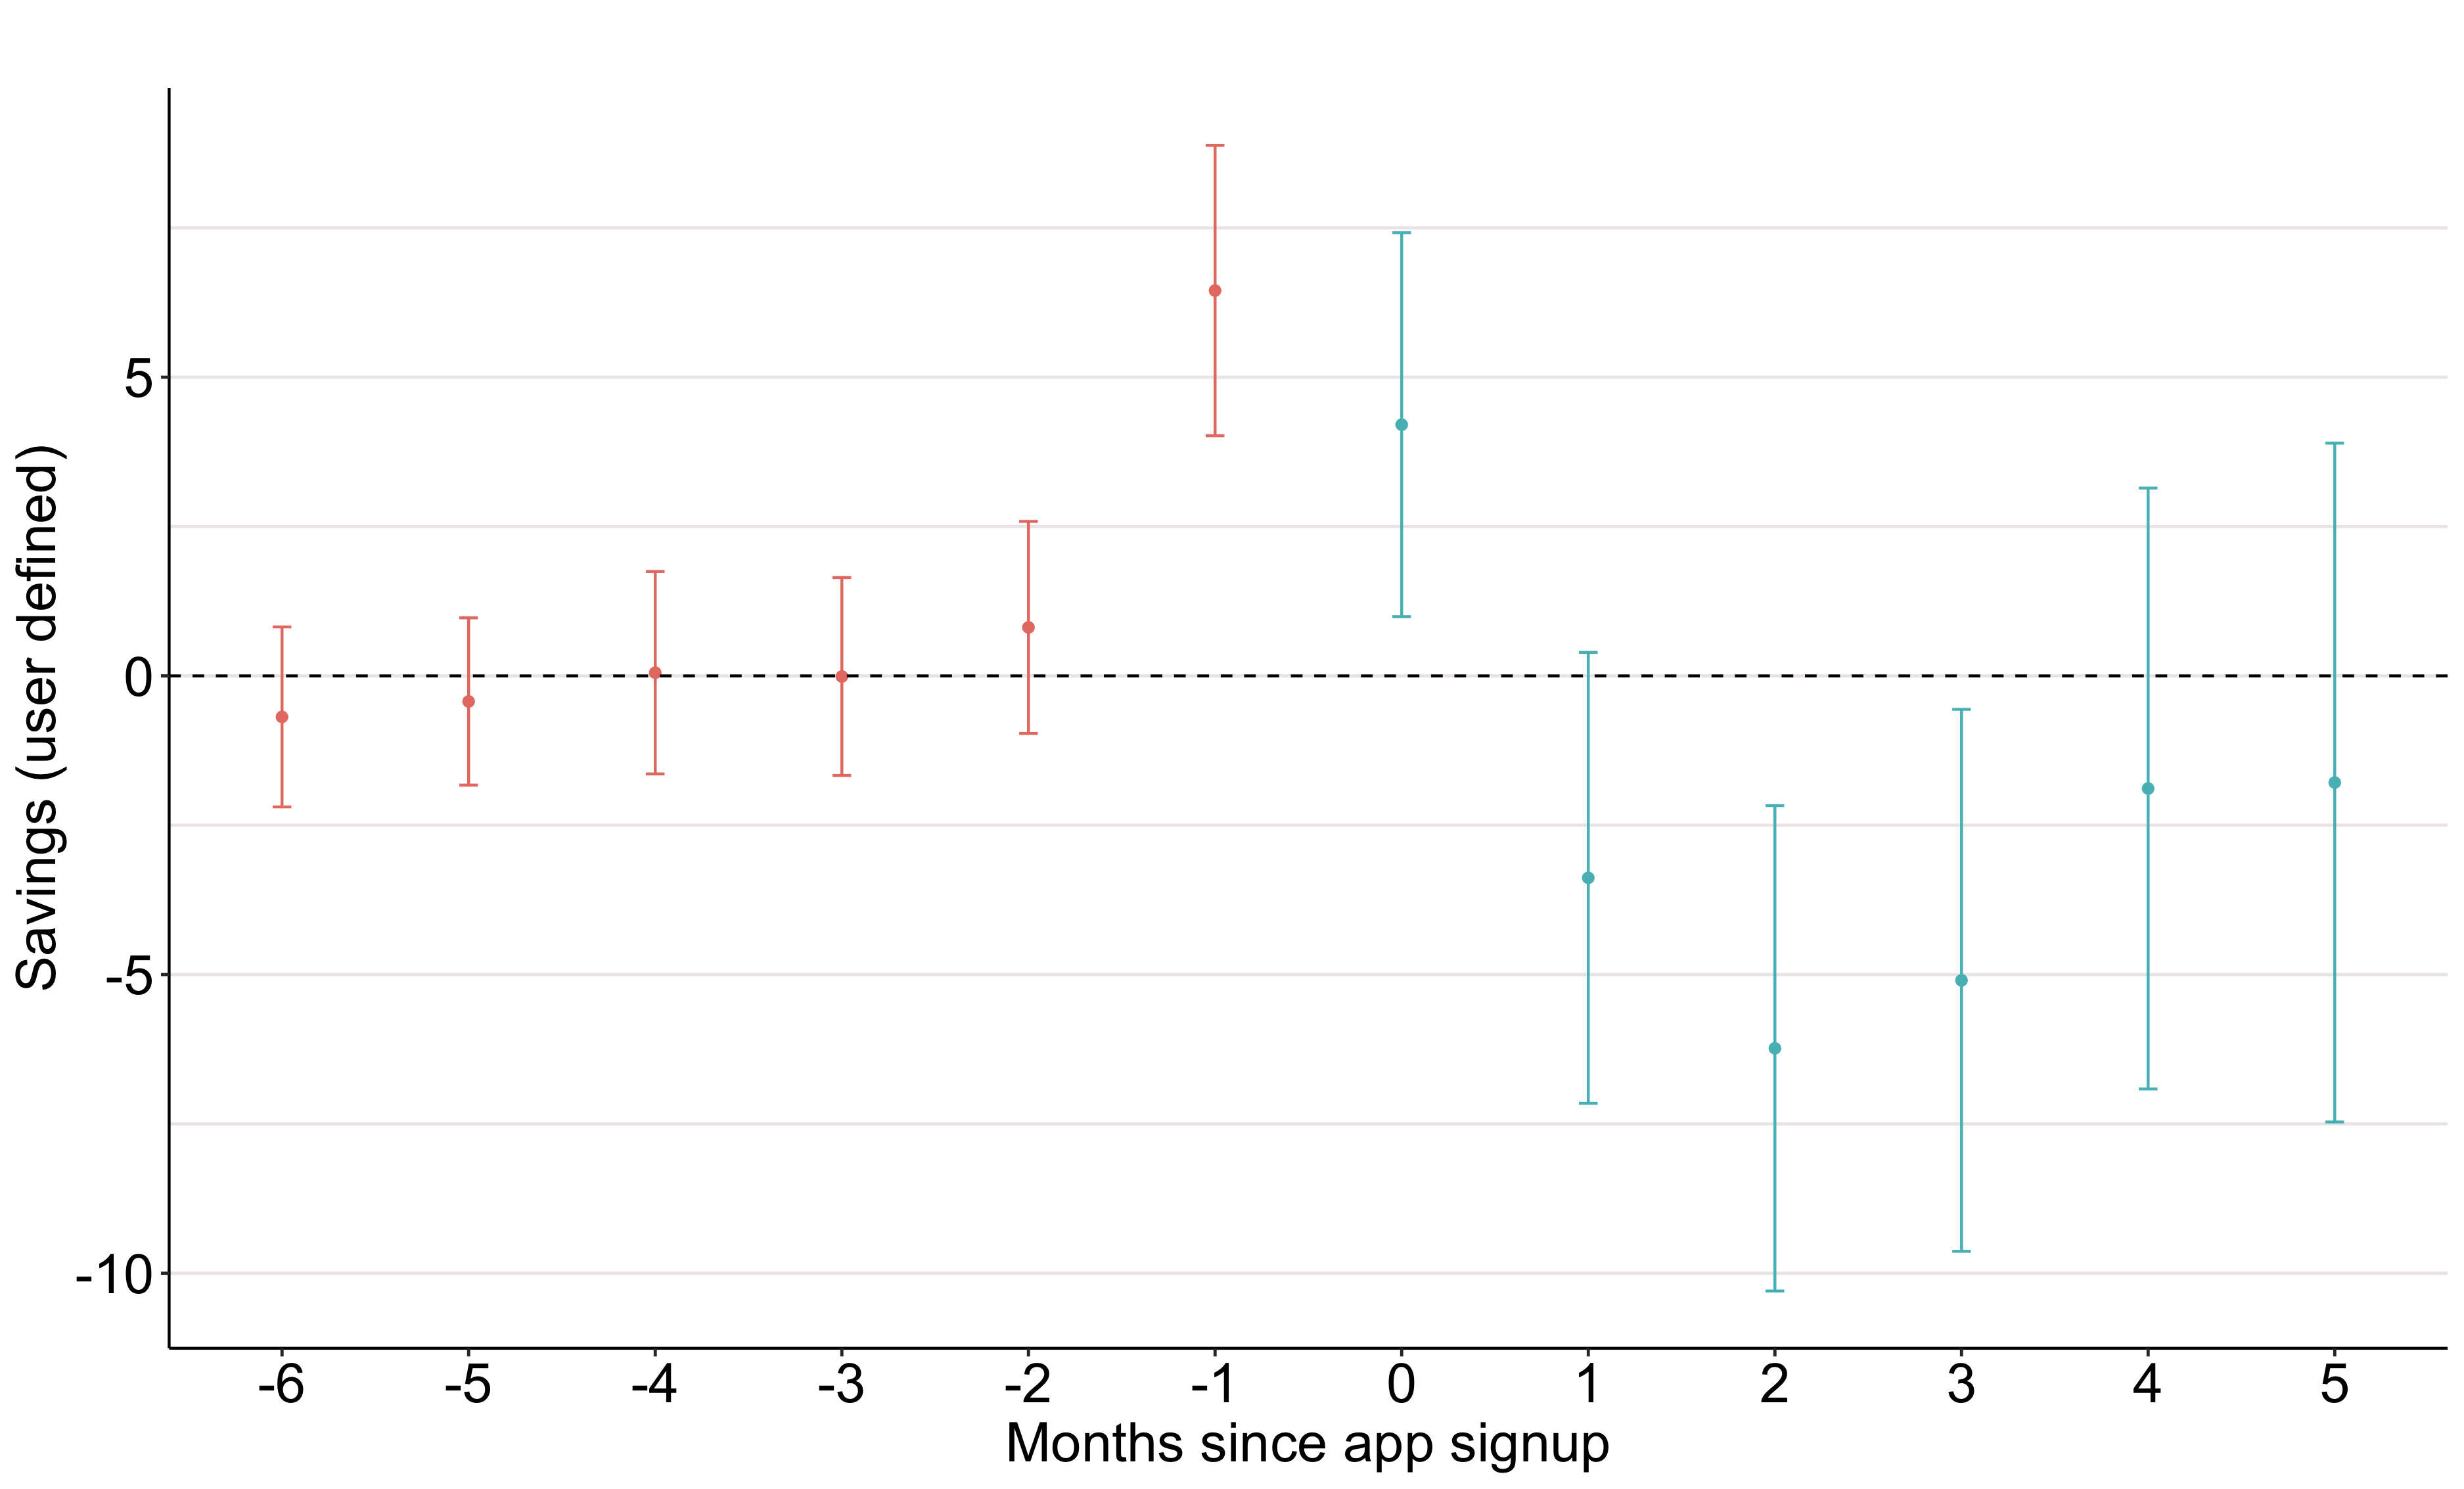
\includegraphics[width=.49\textwidth]{\figdir/up_savings_cond_es.png}
    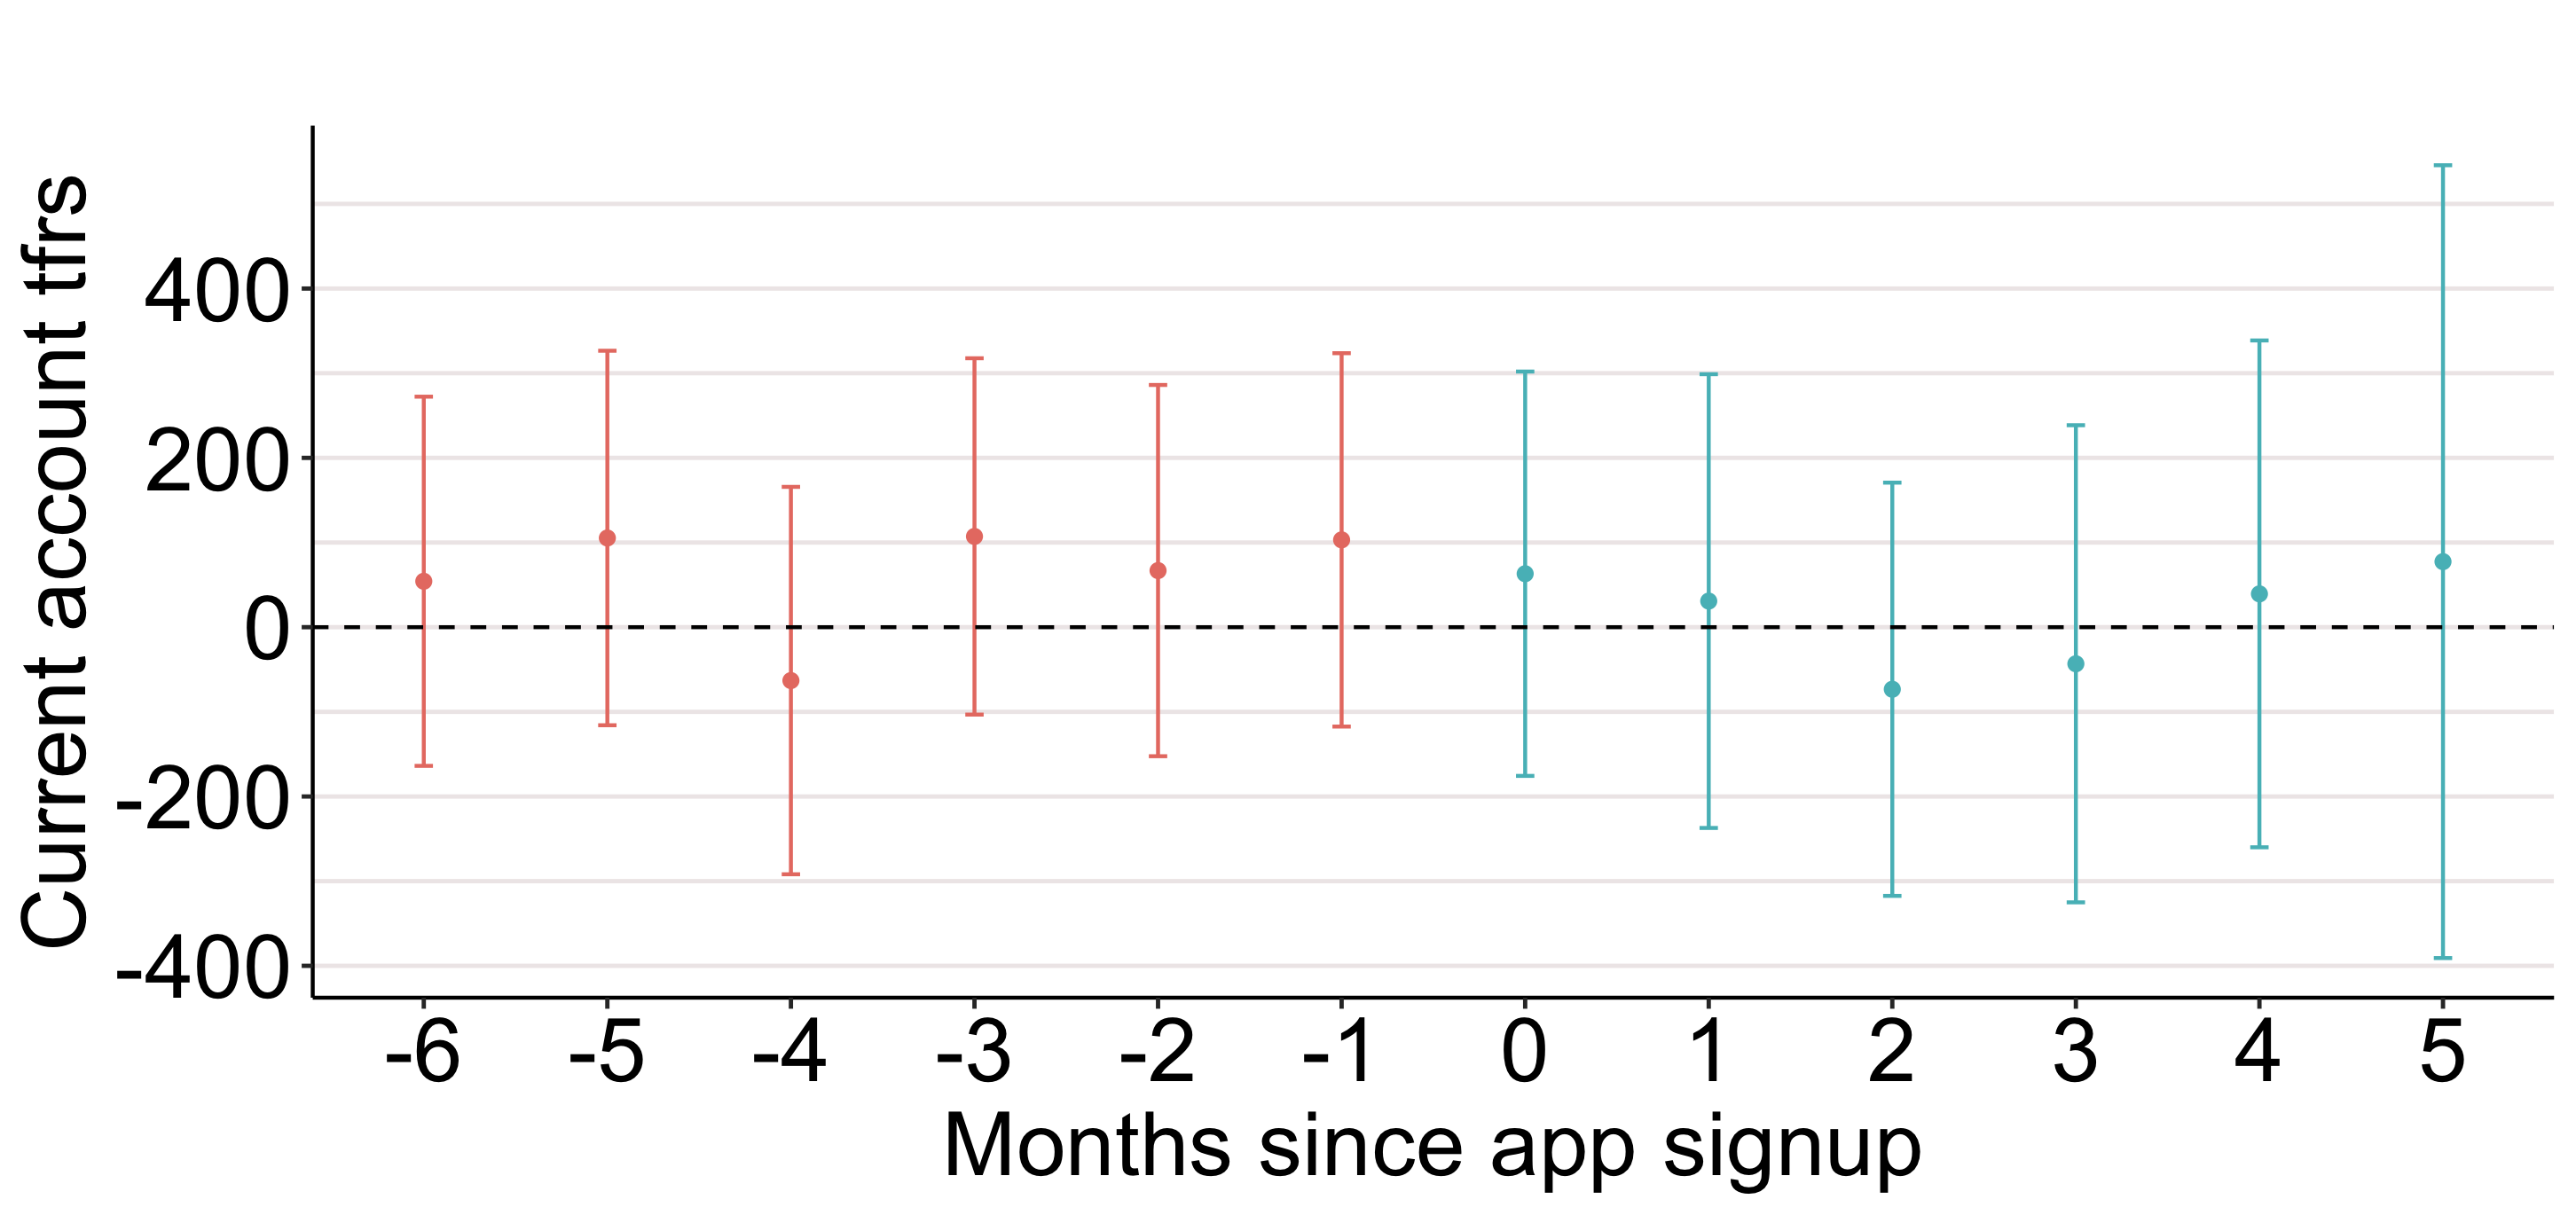
\includegraphics[width=.49\textwidth]{\figdir/ca_transfers_cond_es.png}
    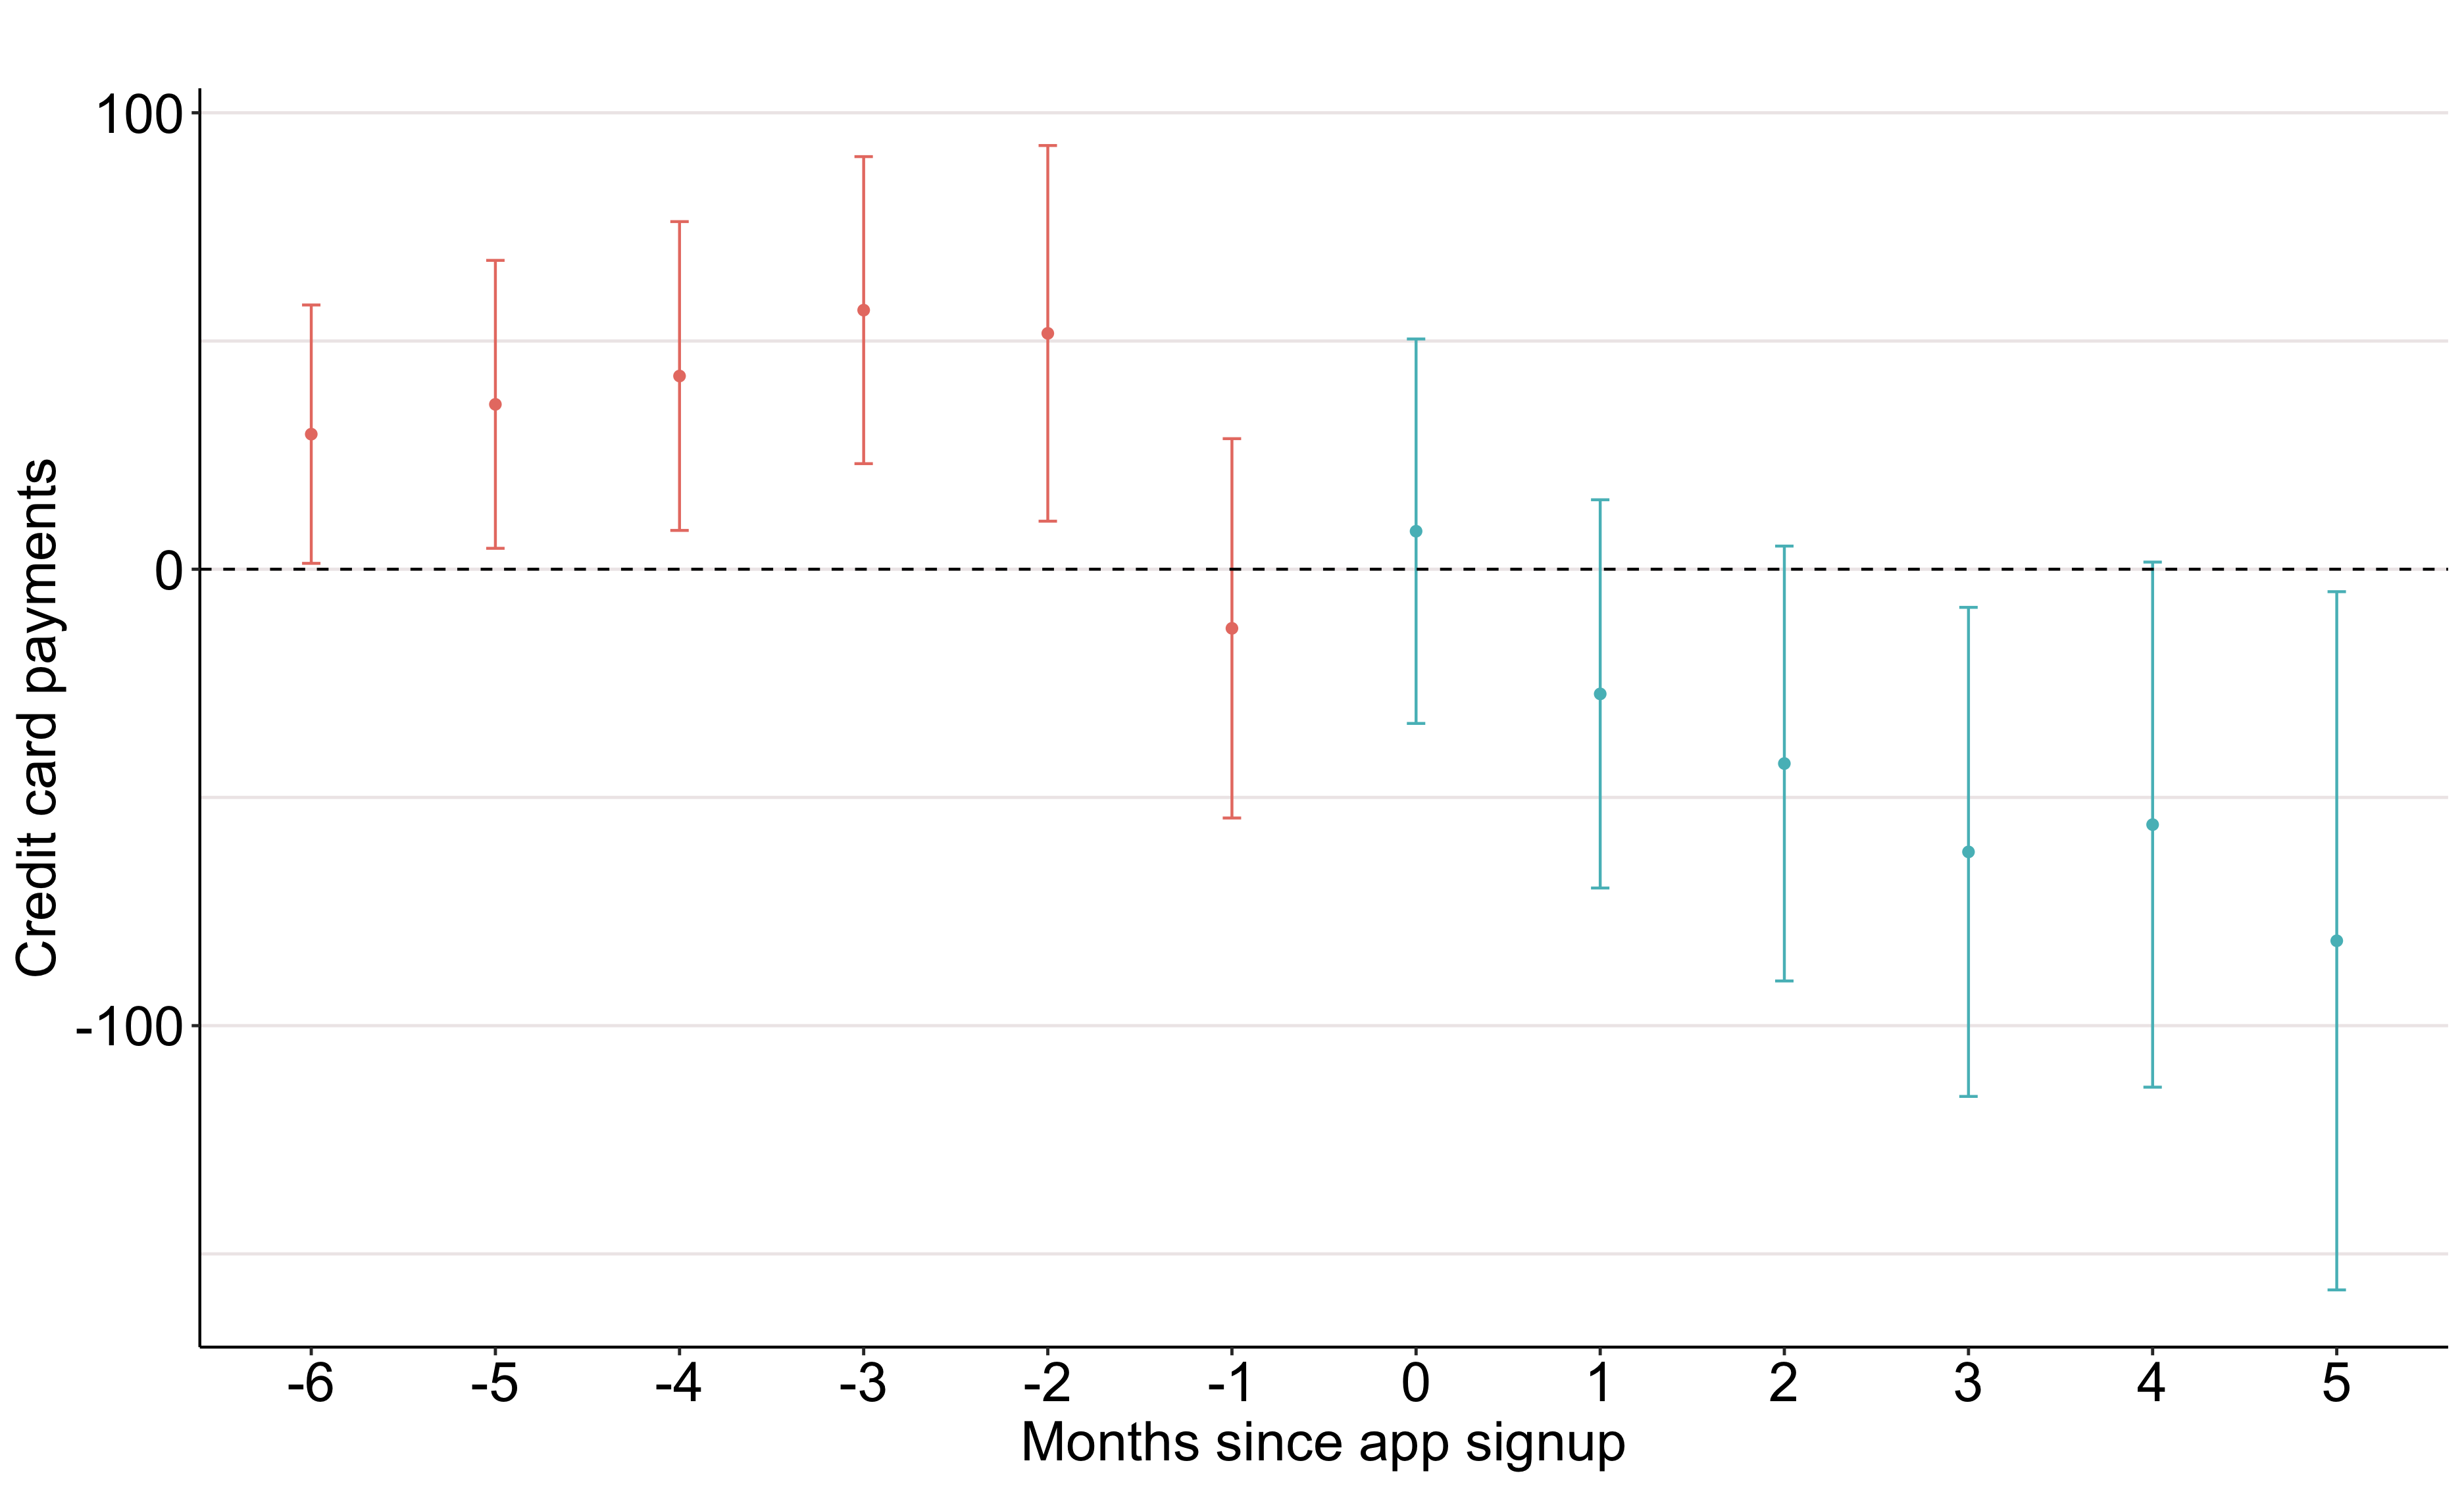
\includegraphics[width=.49\textwidth]{\figdir/cc_payments_cond_es.png}
    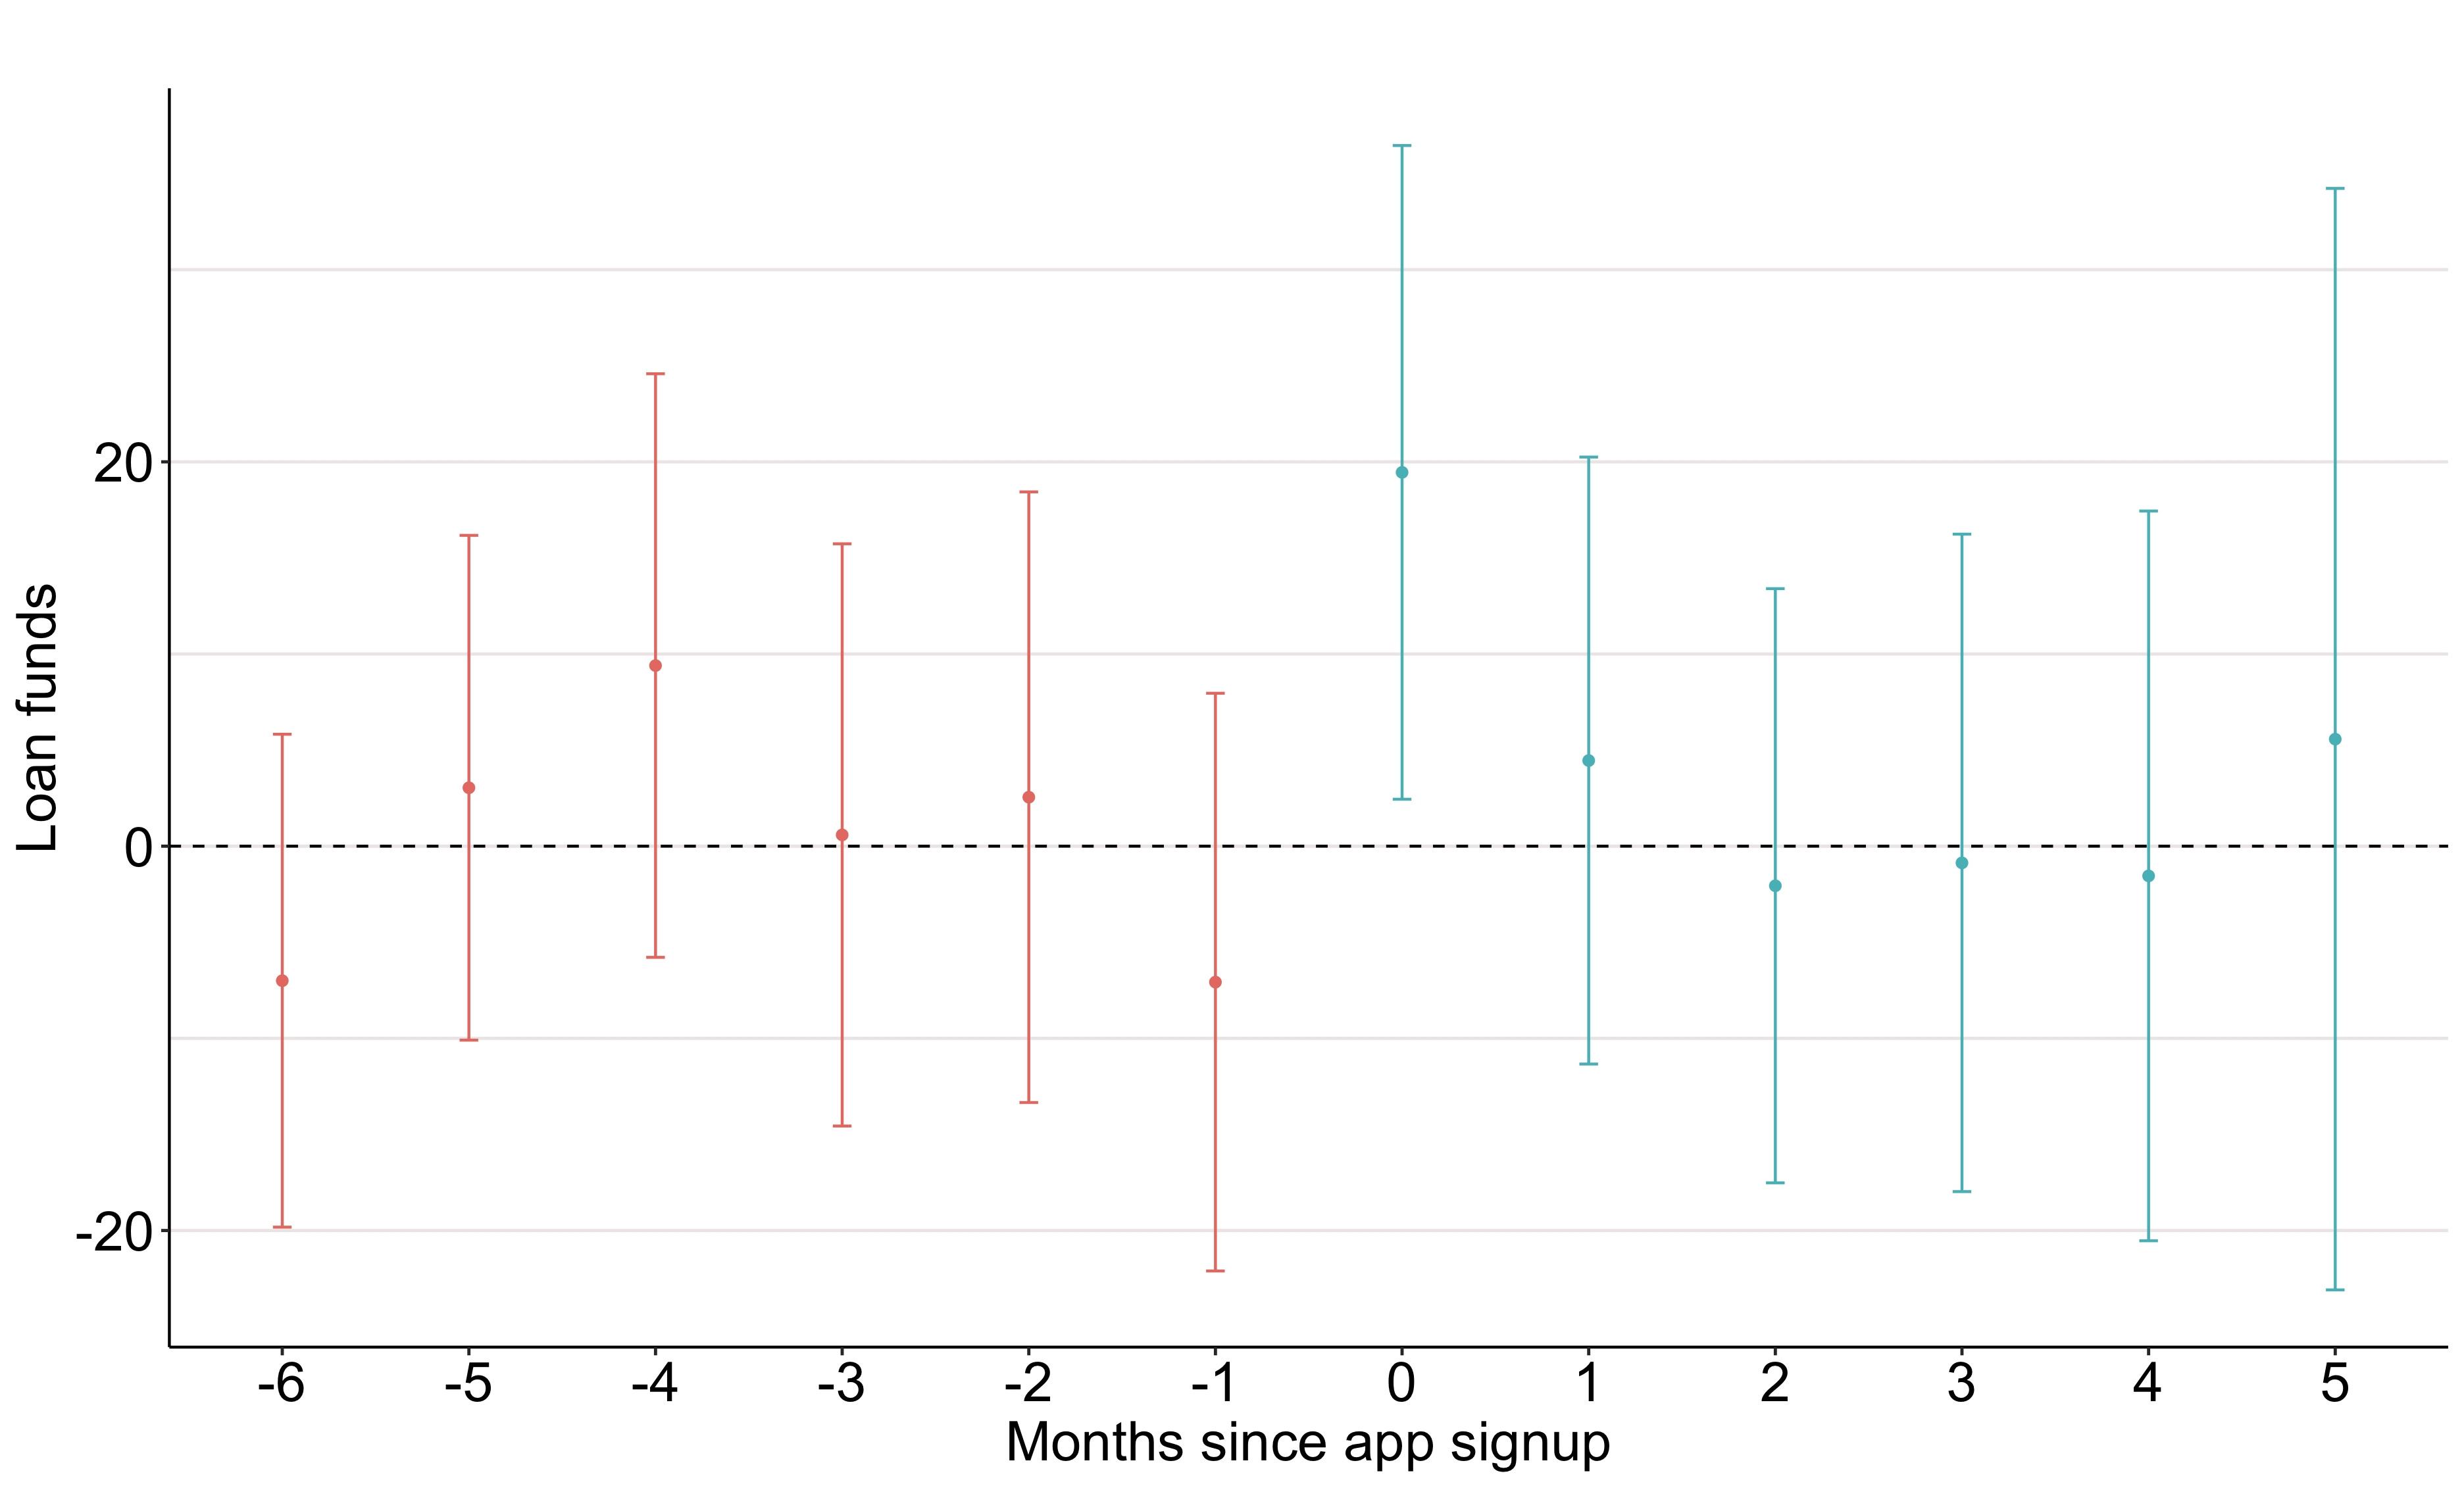
\includegraphics[width=.49\textwidth]{\figdir/loan_funds_cond_es.png}
    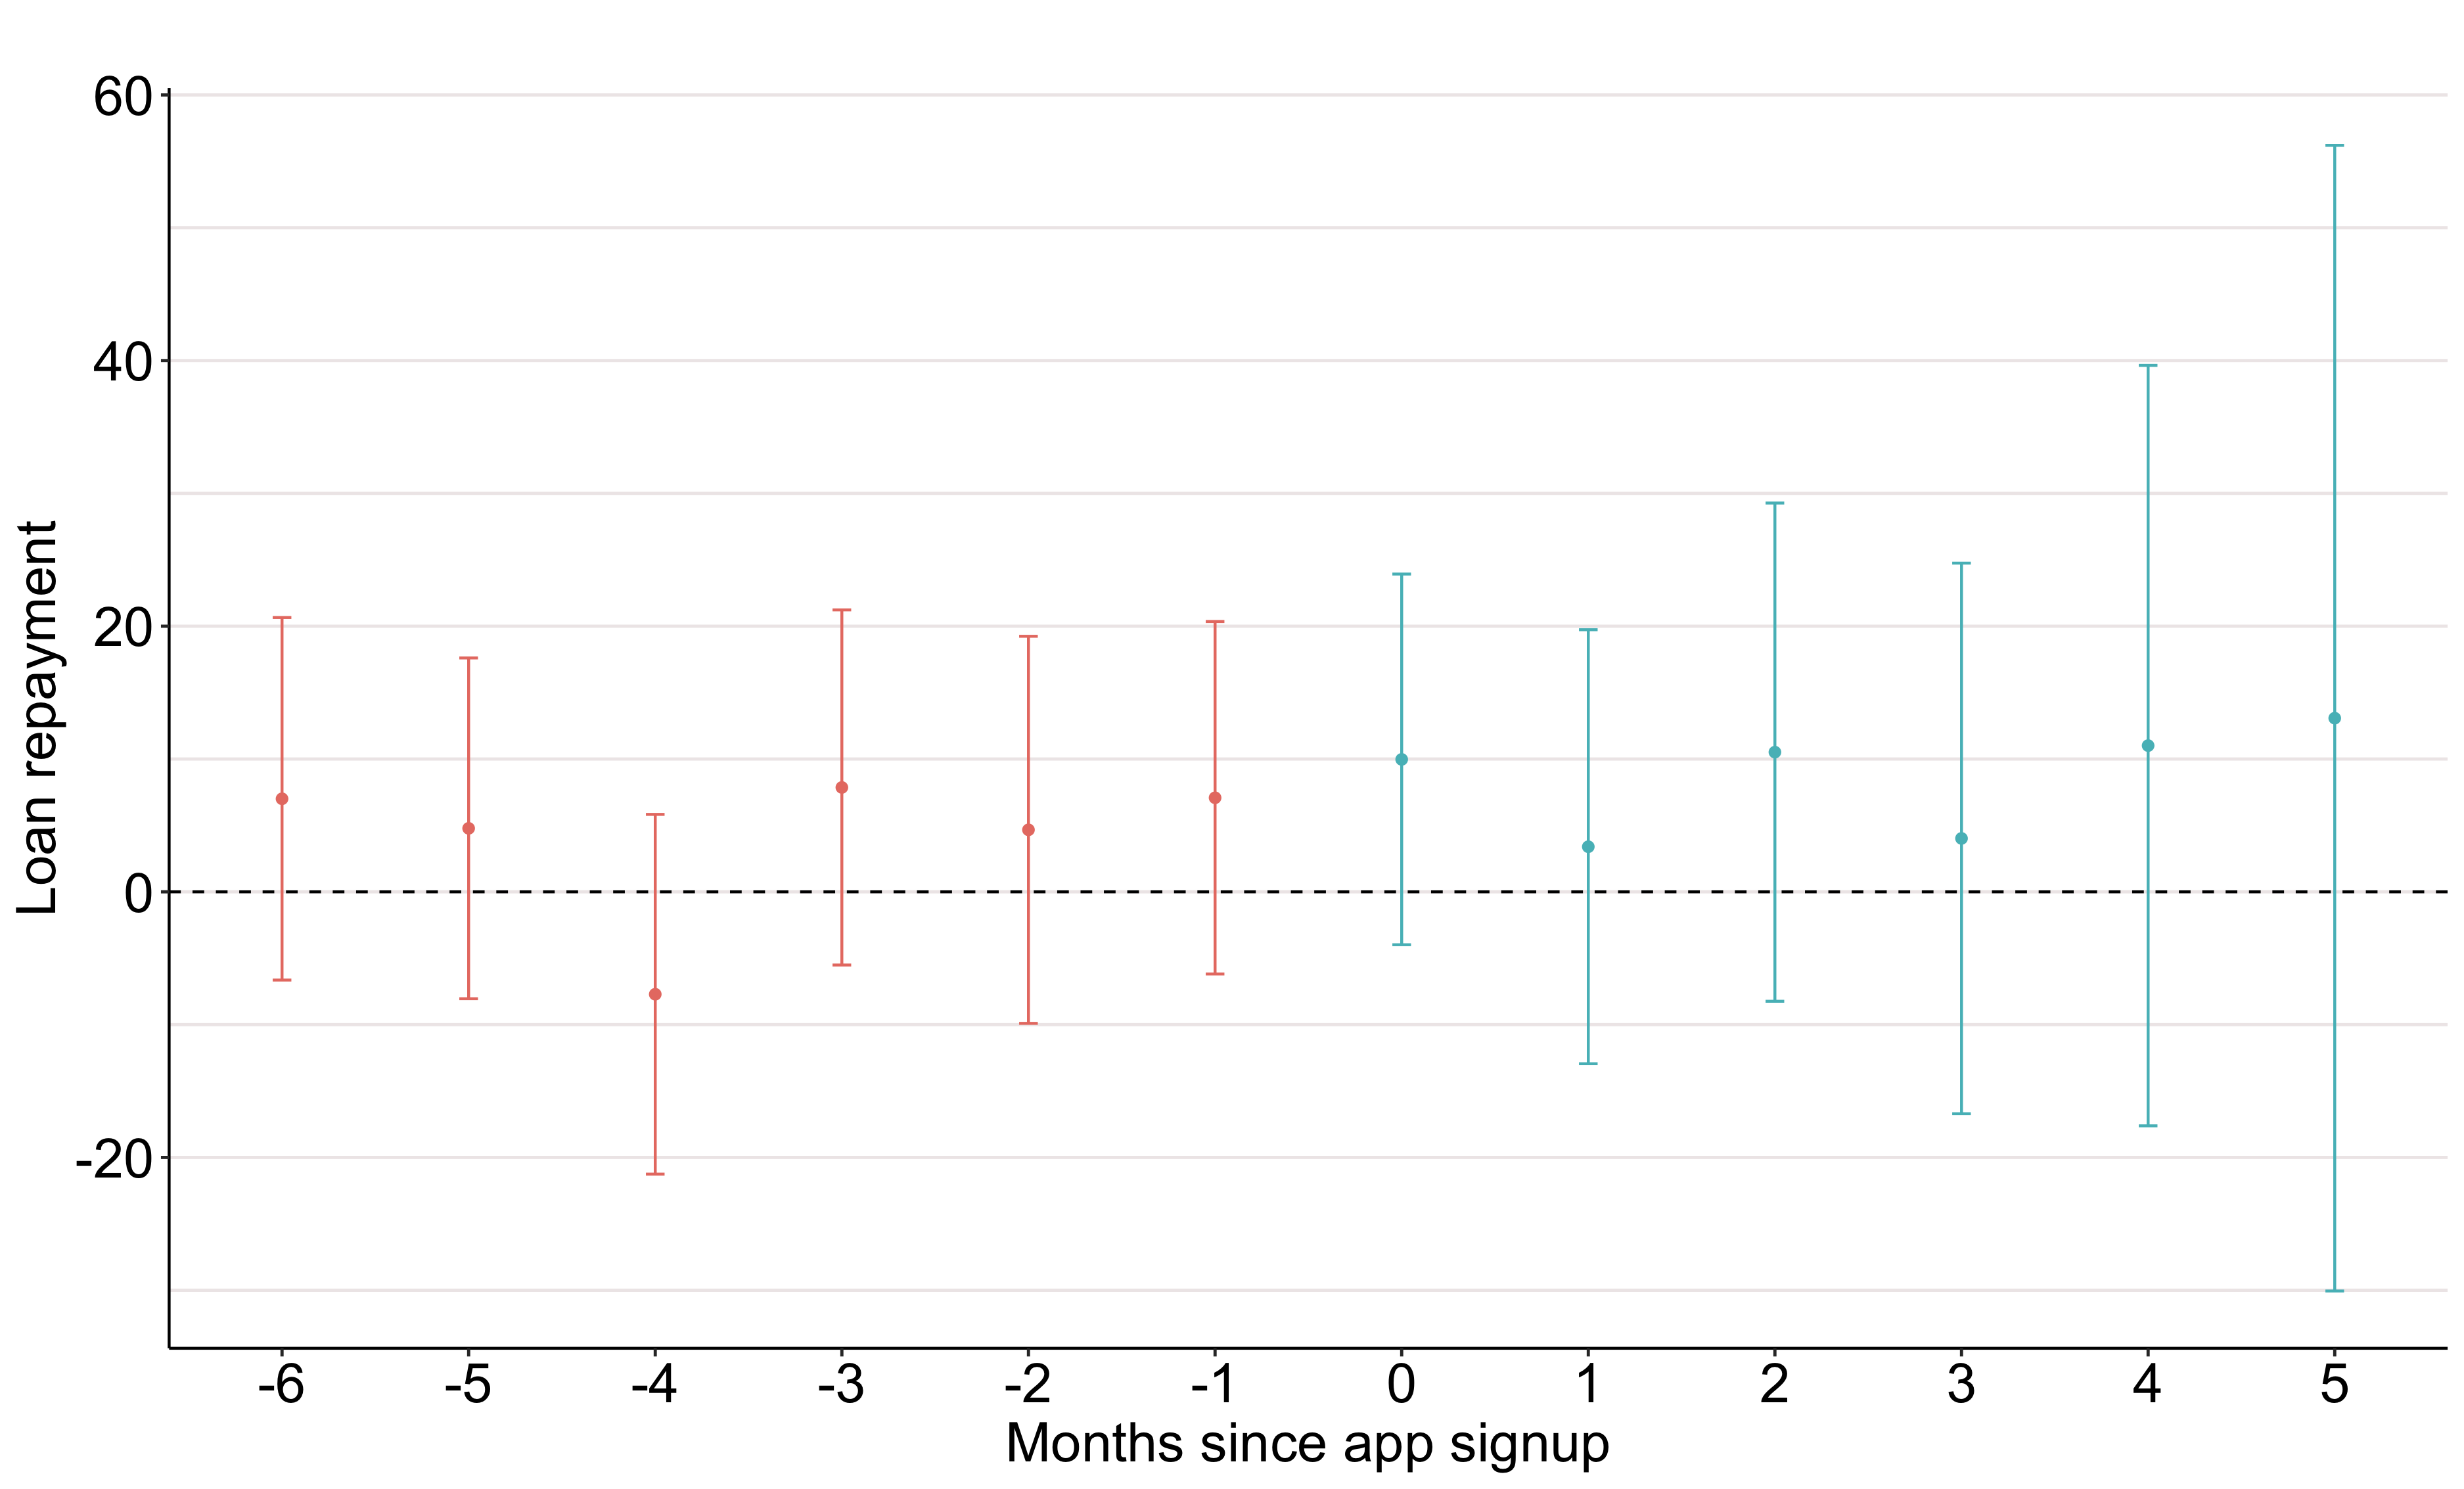
\includegraphics[width=.49\textwidth]{\figdir/loan_rpmts_cond_es.png}
    \fignote{\textwidth}{Point estimates represent
        group-time average treatment effects aggregated to periods since
        treatment exposure, as defined in Section~\ref{sub:estimation}. Red
        lines represent point estimates and uniform 95\% confidence bands for
        pre-treatment periods allowing for clustering at the user level. If the
        null hypothesis that parallel trends hold in all periods is correct,
        these should be equal to zero. Blue lines provide similar information
    for post-treatment periods.}
\end{figure}


\subsection{Repeated vs one-off reduction in discretionary spend}%
\label{sub:repeated_vs_one_off_reduction_in_discretionary_spend}

\begin{itemize}
    \item 
\end{itemize}
\begin{figure}[H]
    \centering
    \caption{Disaggregated discretionary spend}%
    \label{fig:disagg_dspend}
    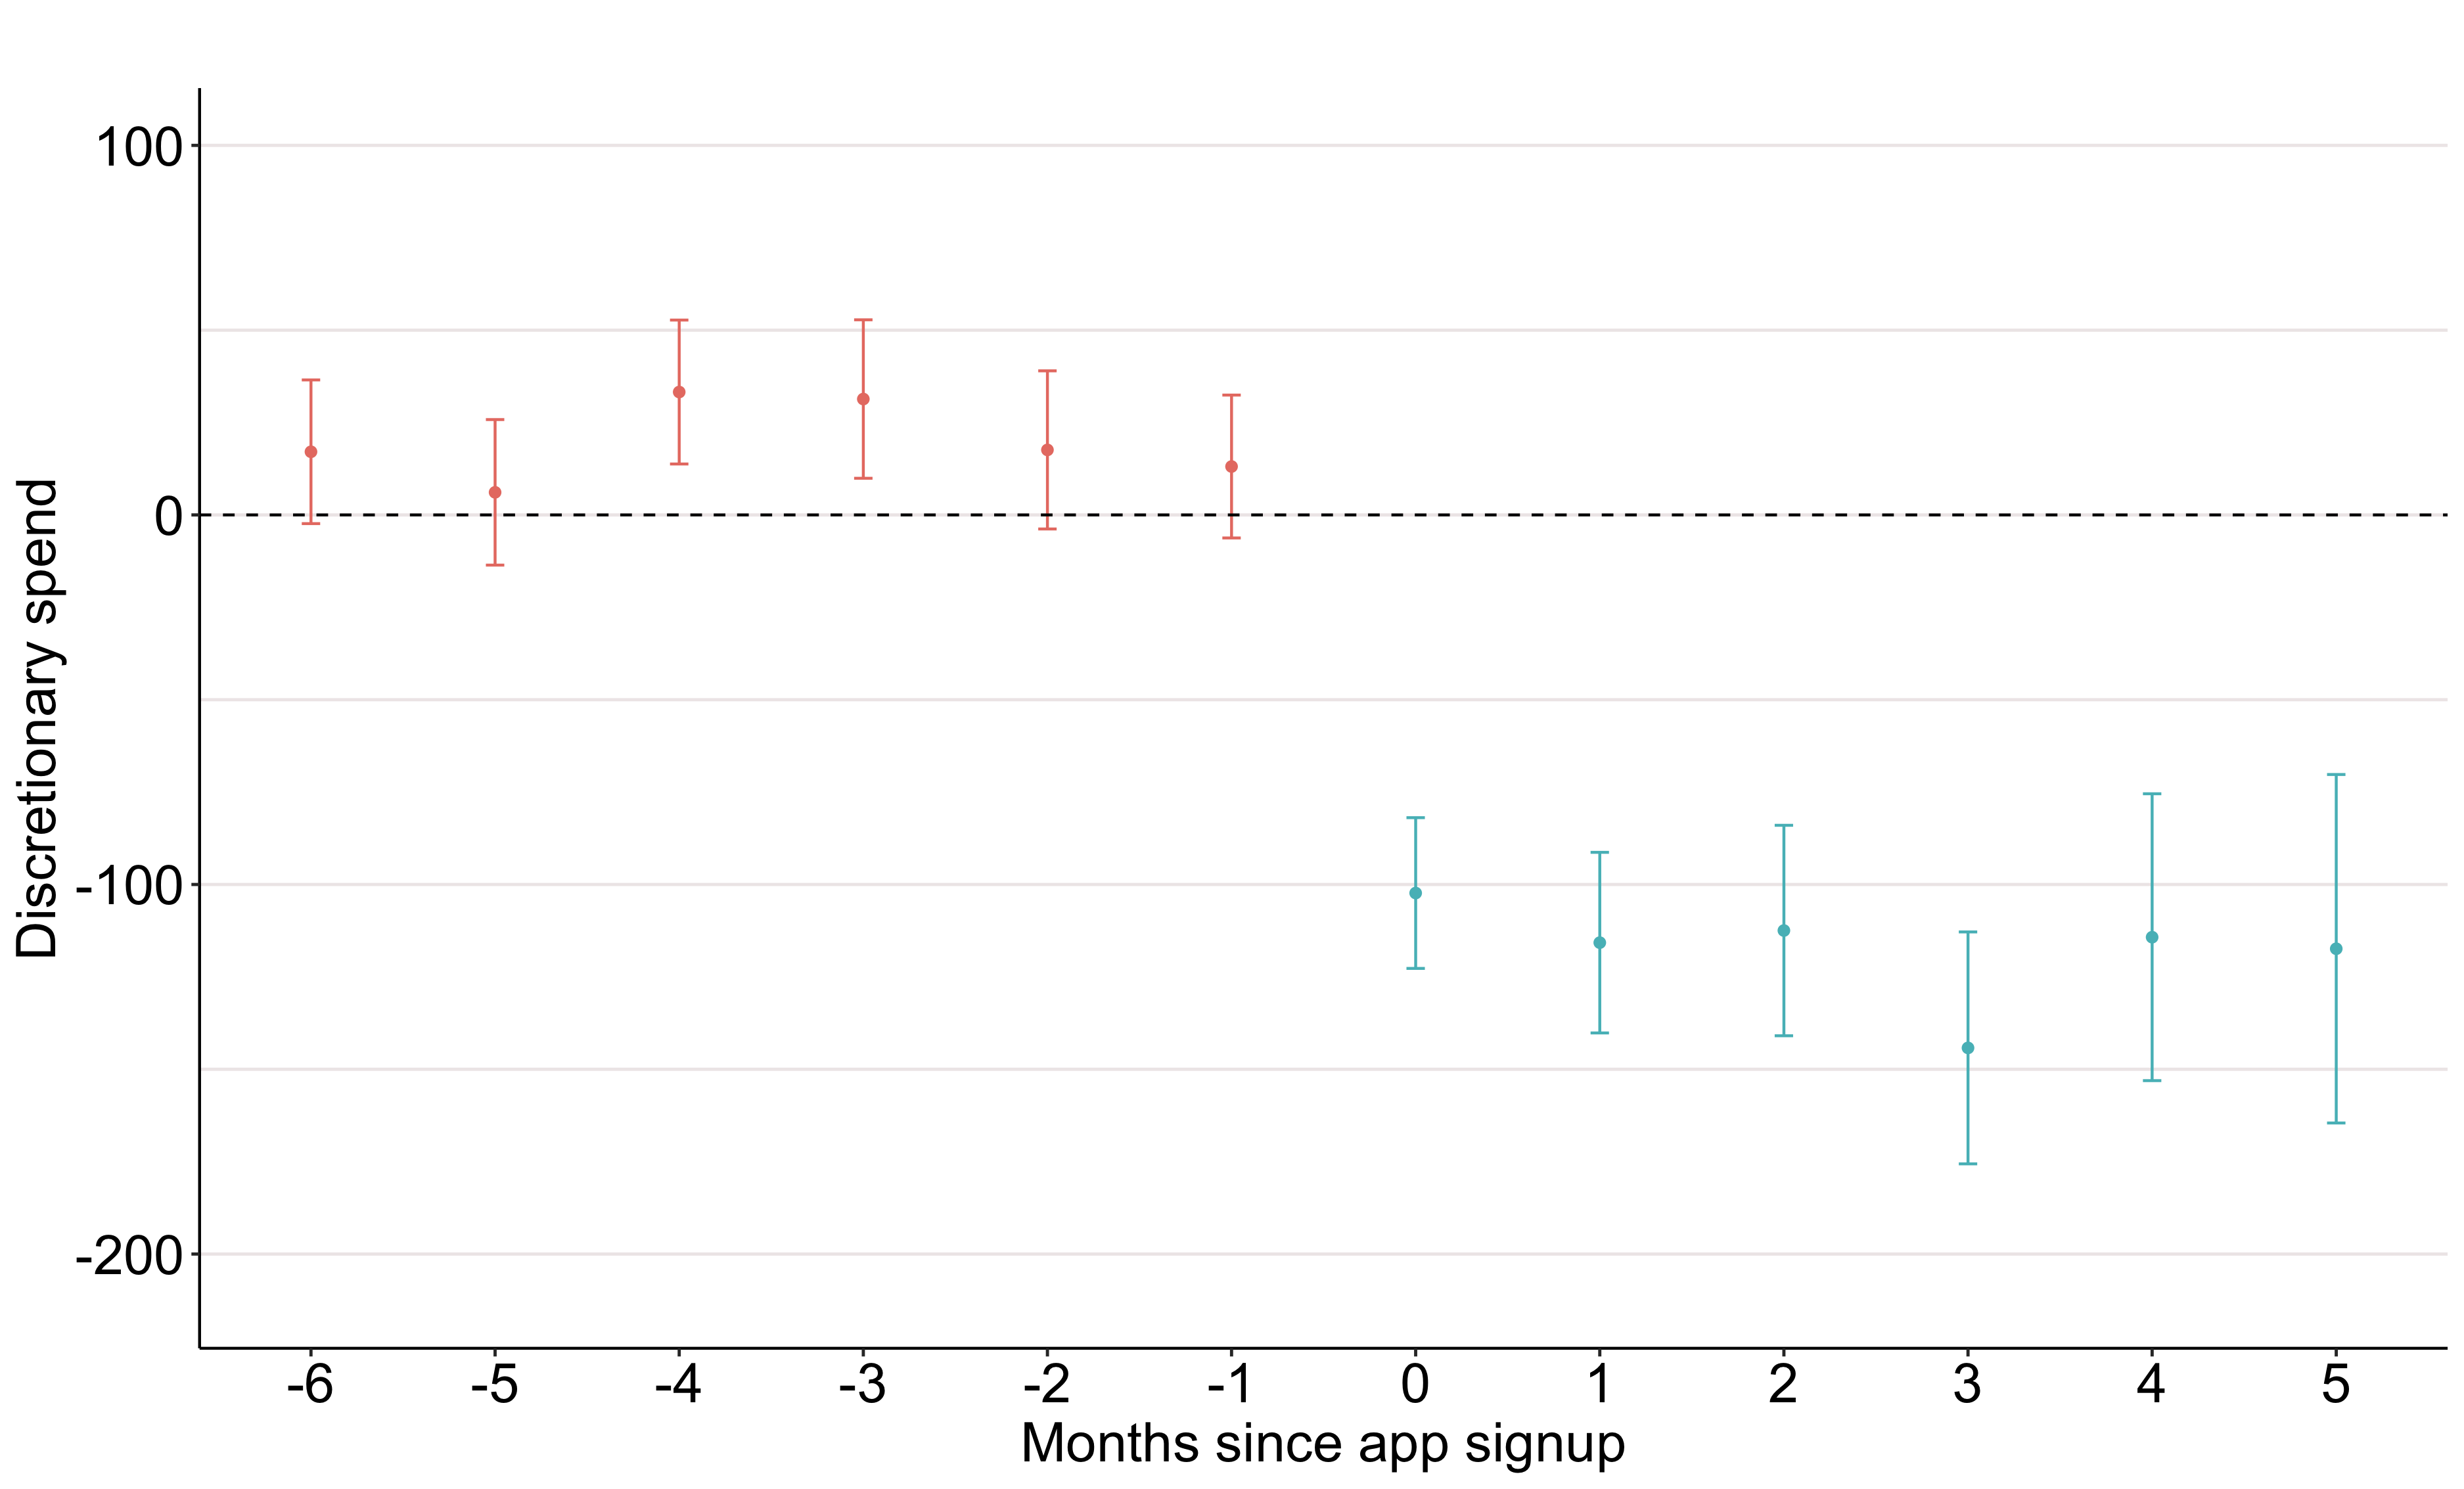
\includegraphics[width=.49\textwidth]{\figdir/disag_dspend_cond_es.png}
    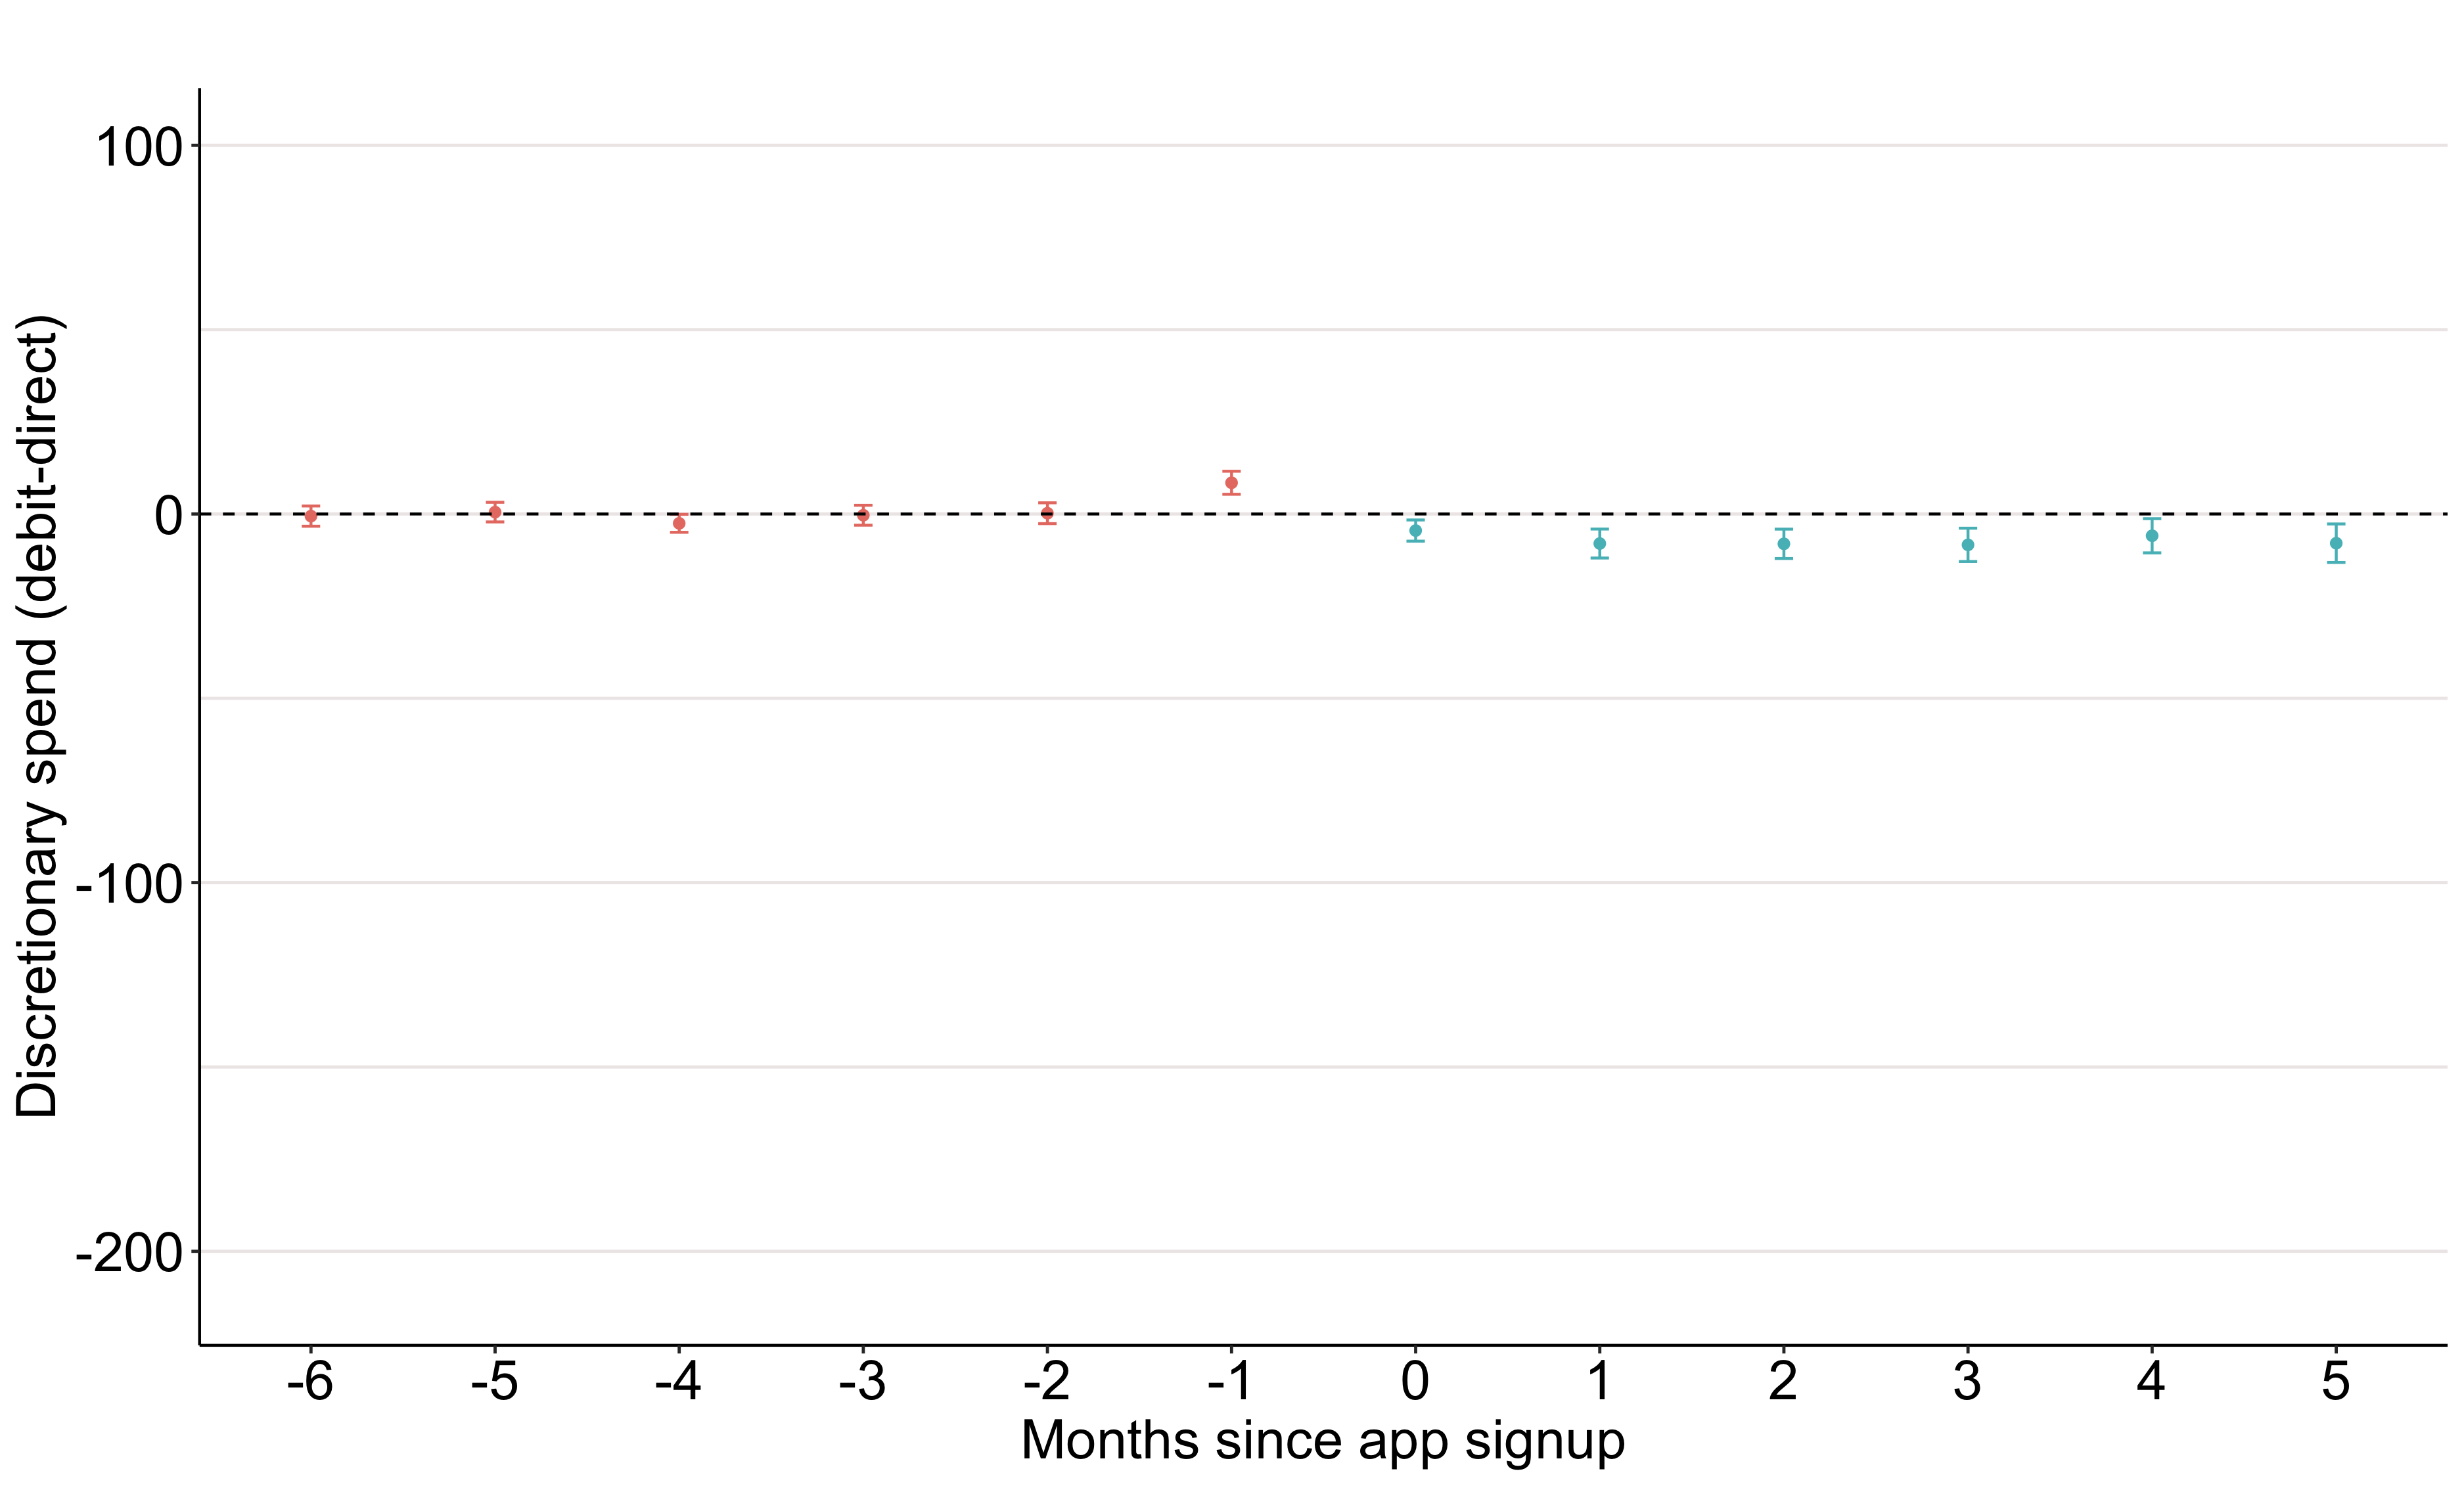
\includegraphics[width=.49\textwidth]{\figdir/disag_dspend_dd_cond_es.png}
    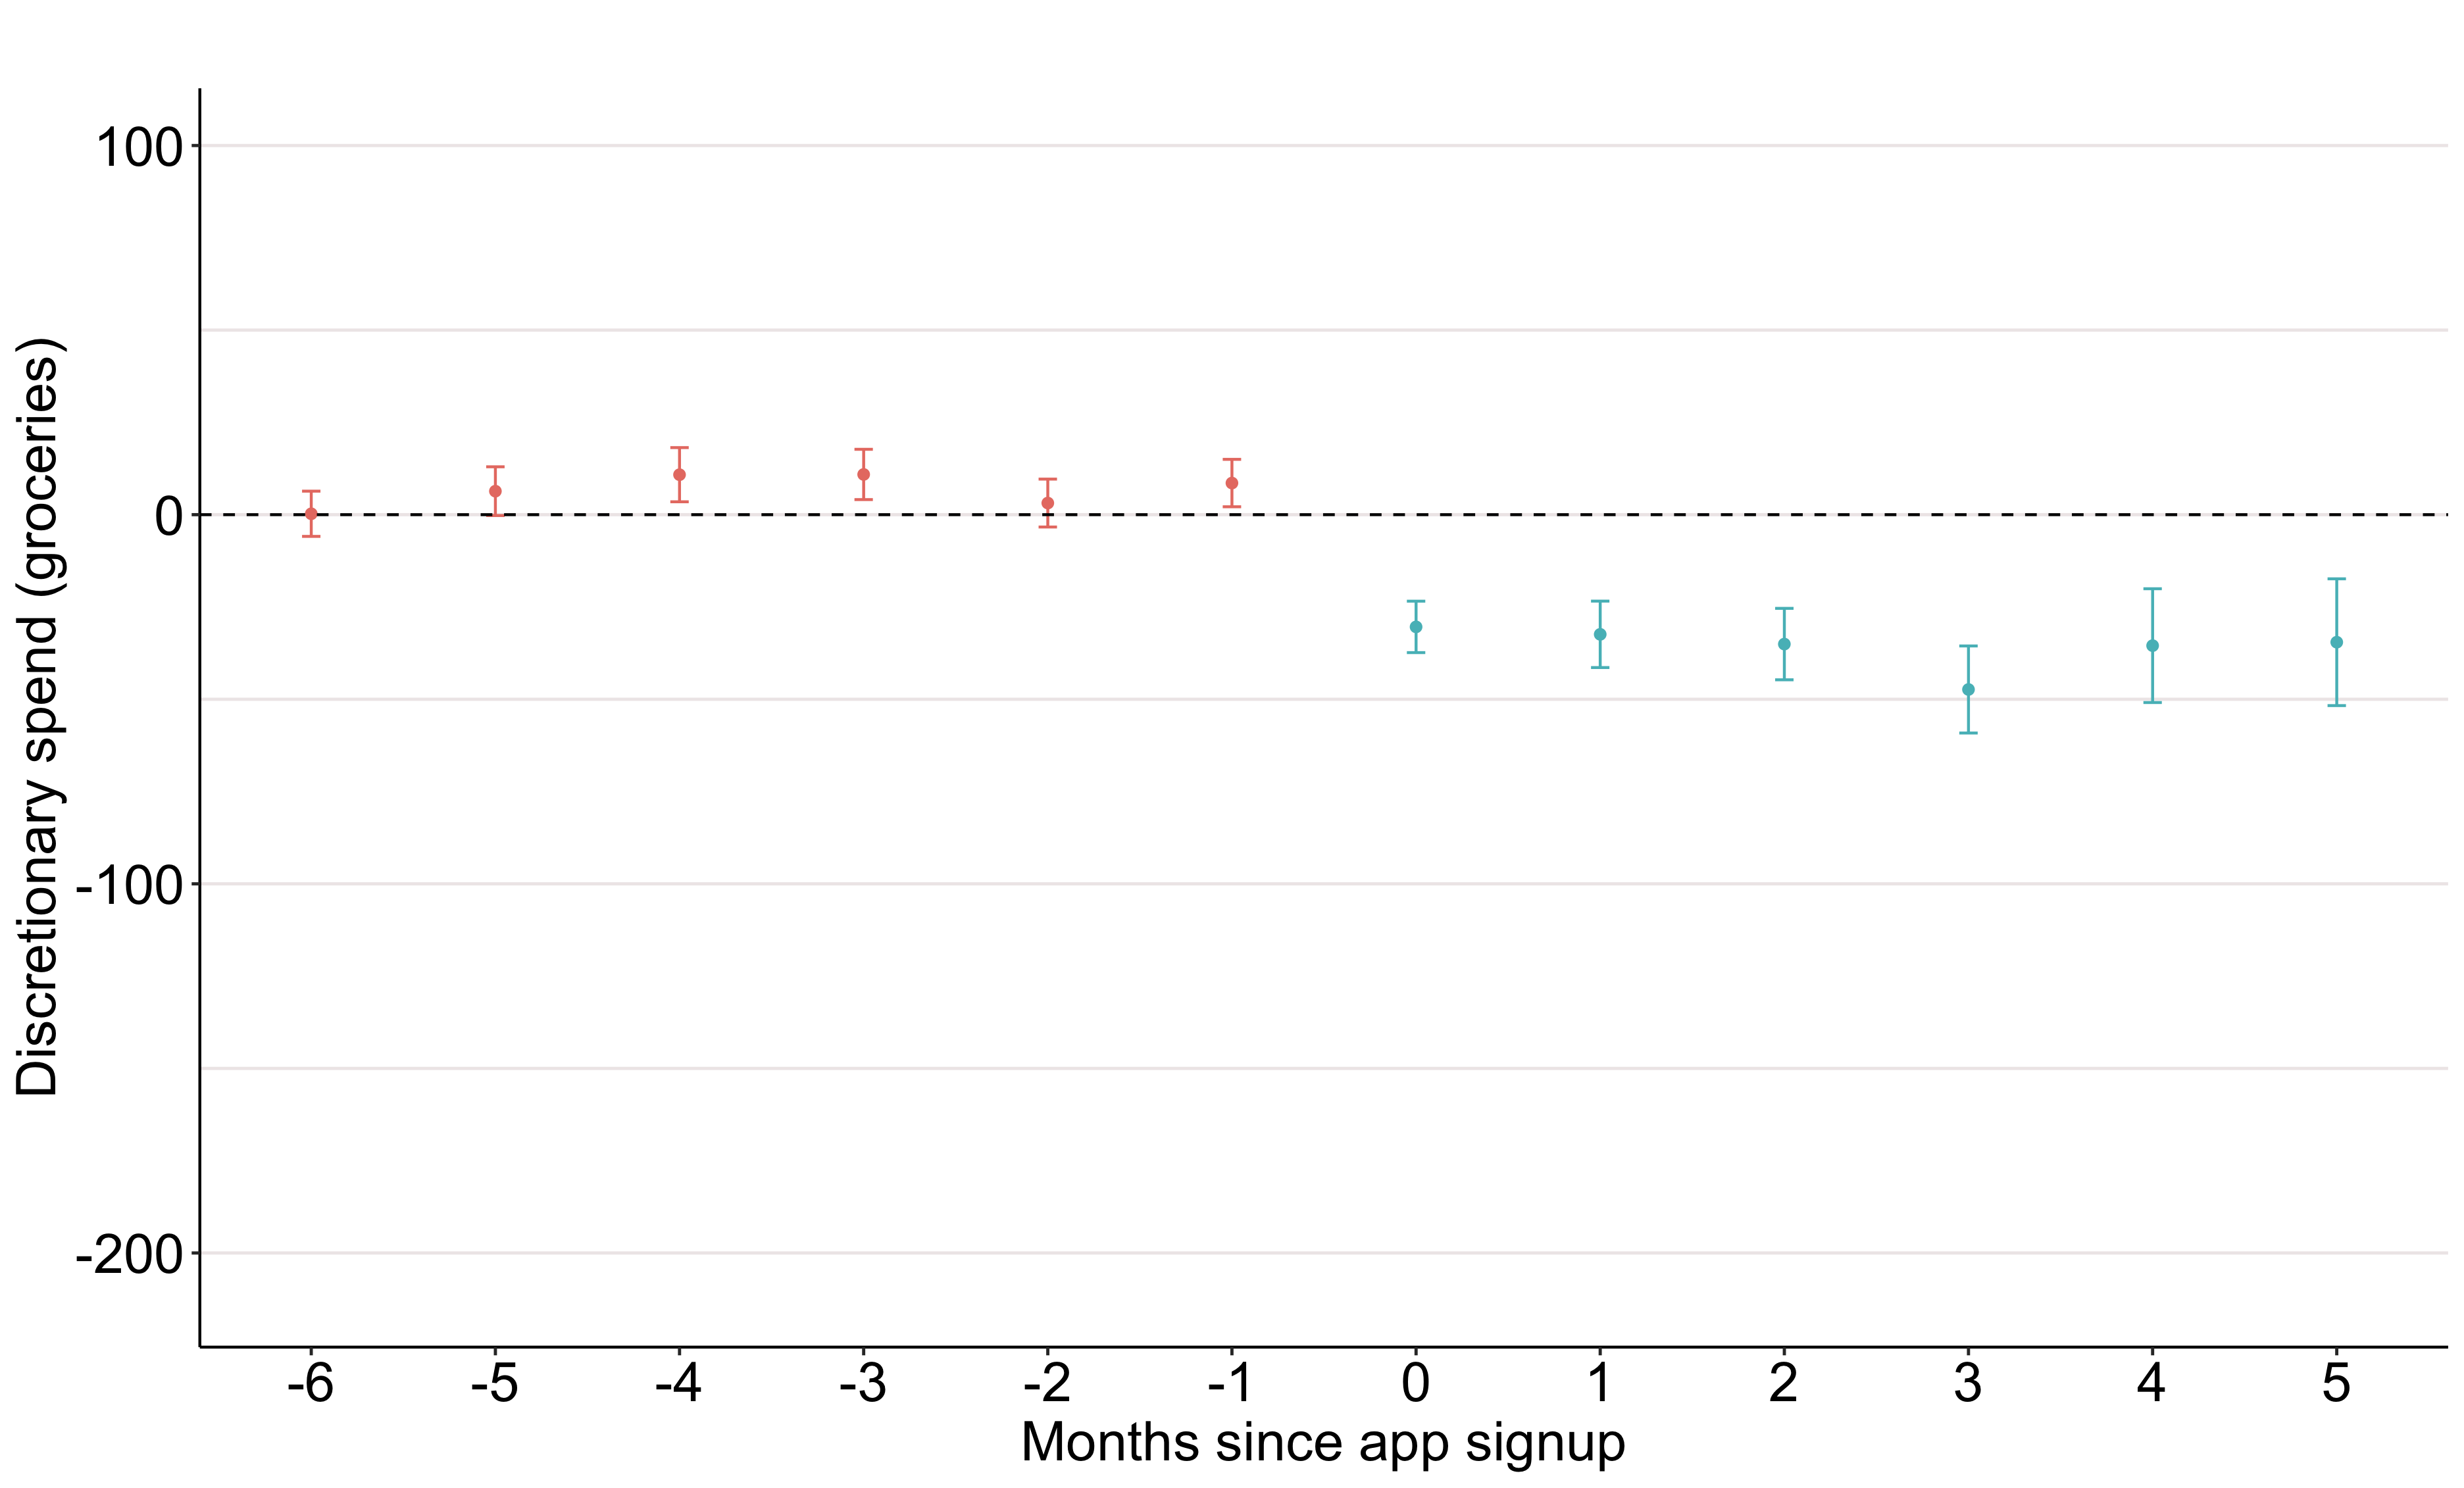
\includegraphics[width=.49\textwidth]{\figdir/disag_dspend_groceries_cond_es.png}
    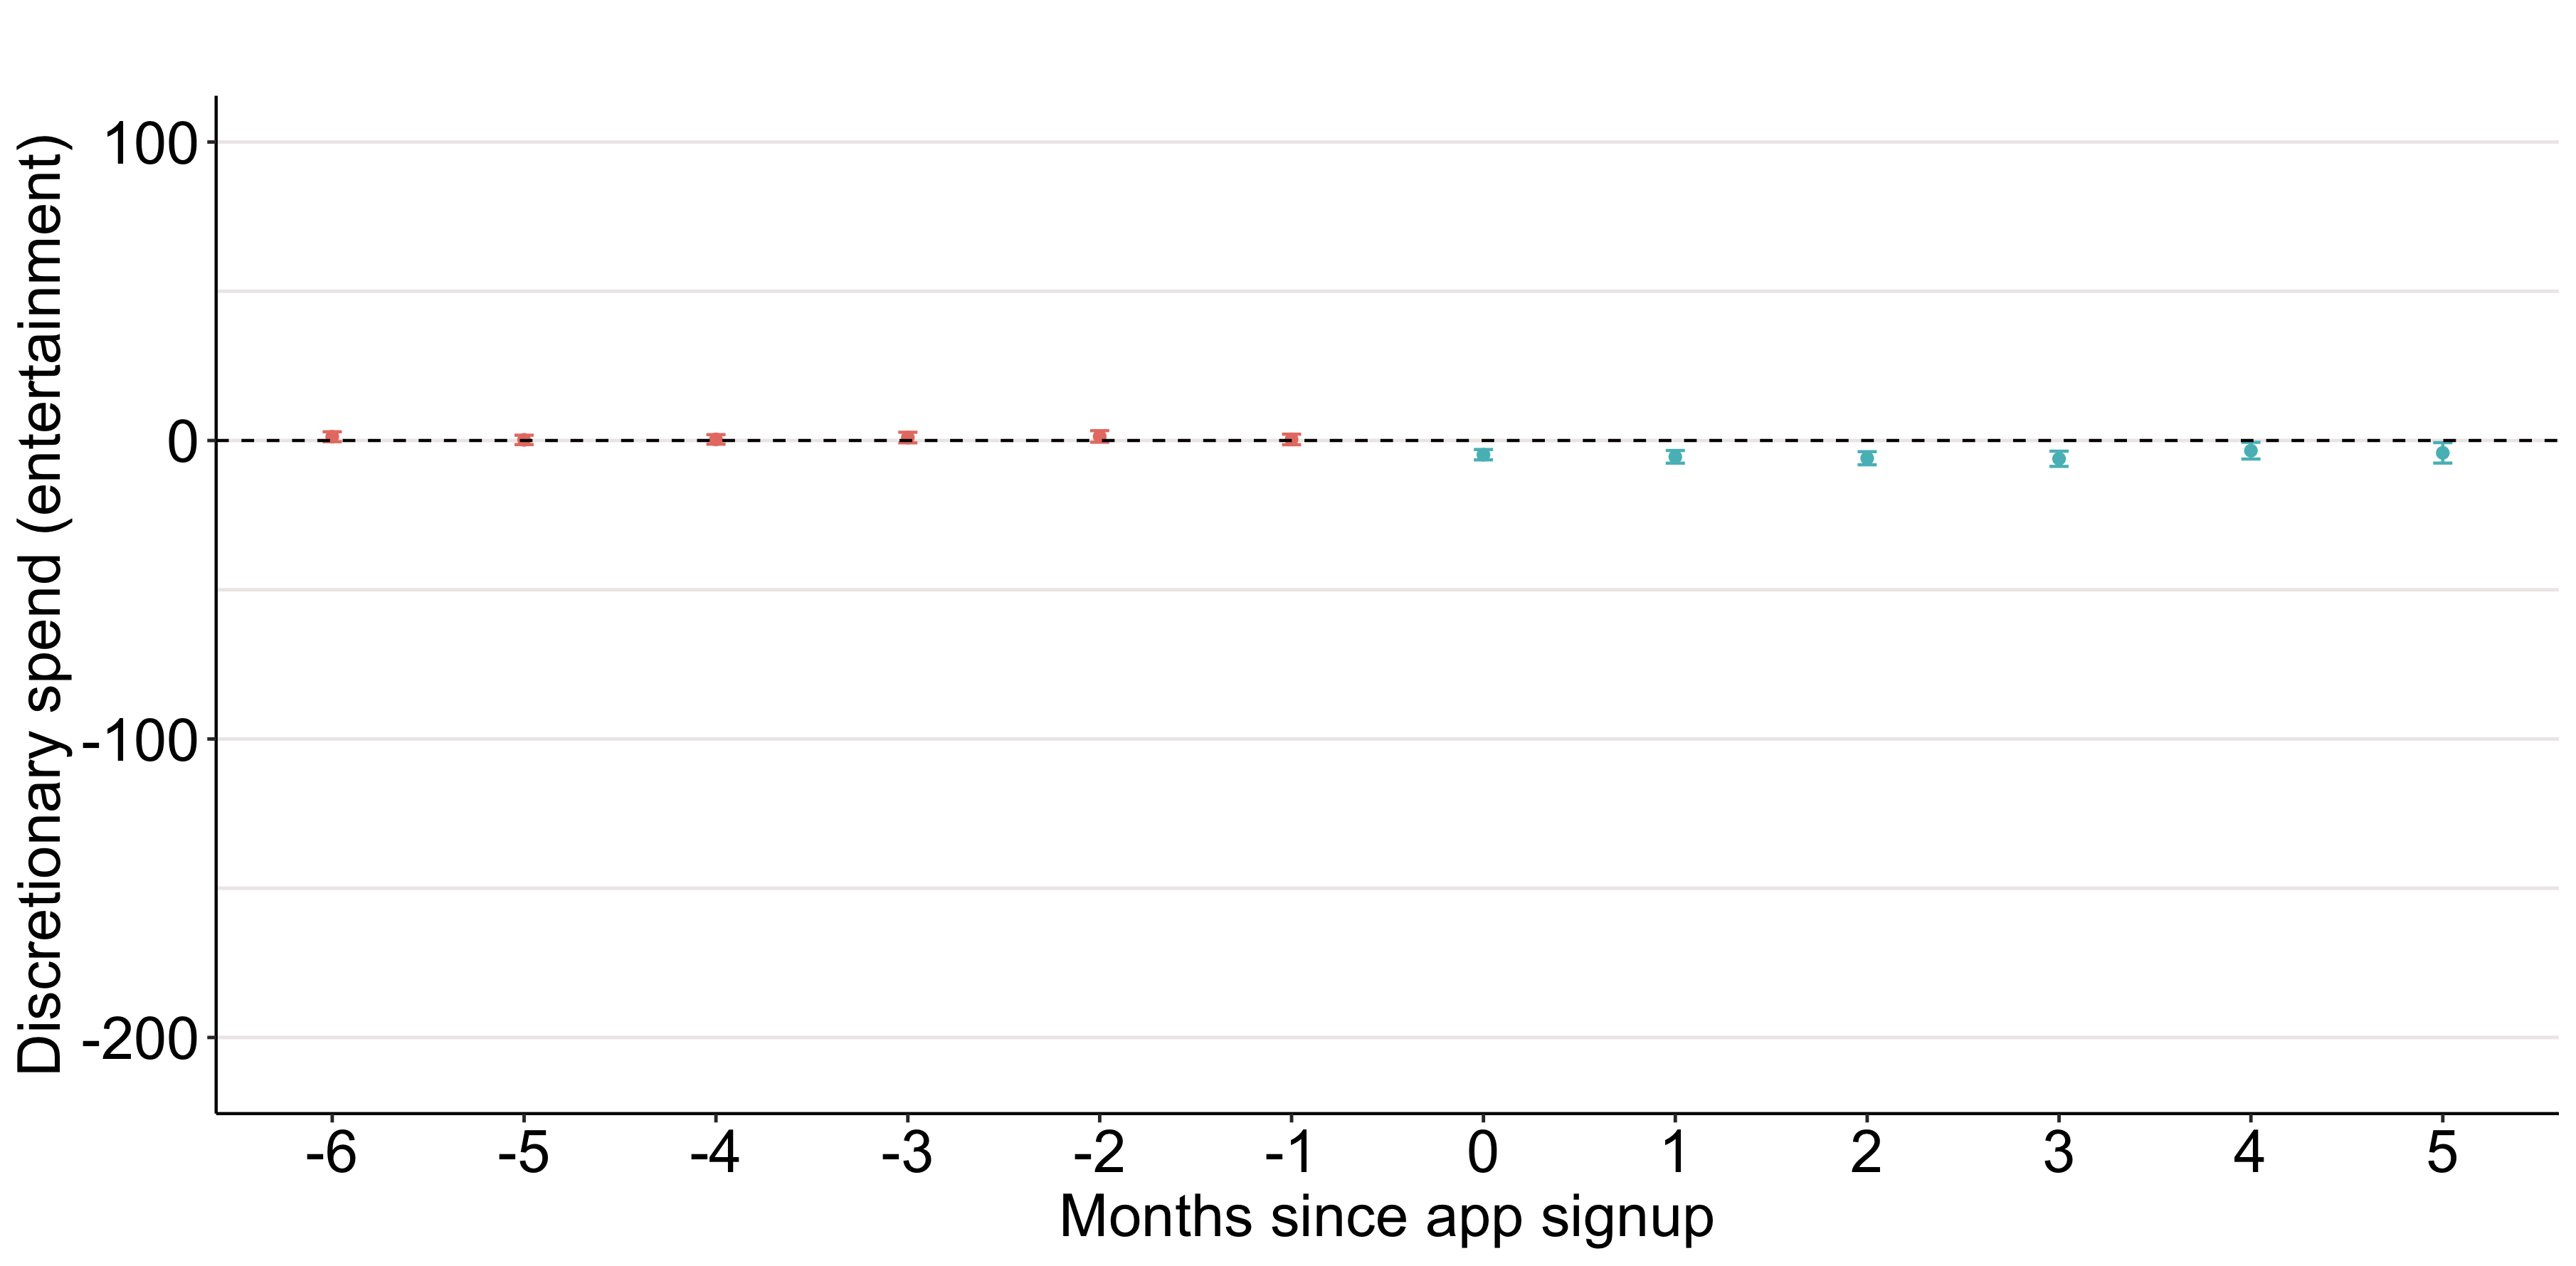
\includegraphics[width=.49\textwidth]{\figdir/disag_dspend_entertainment_cond_es.png}
    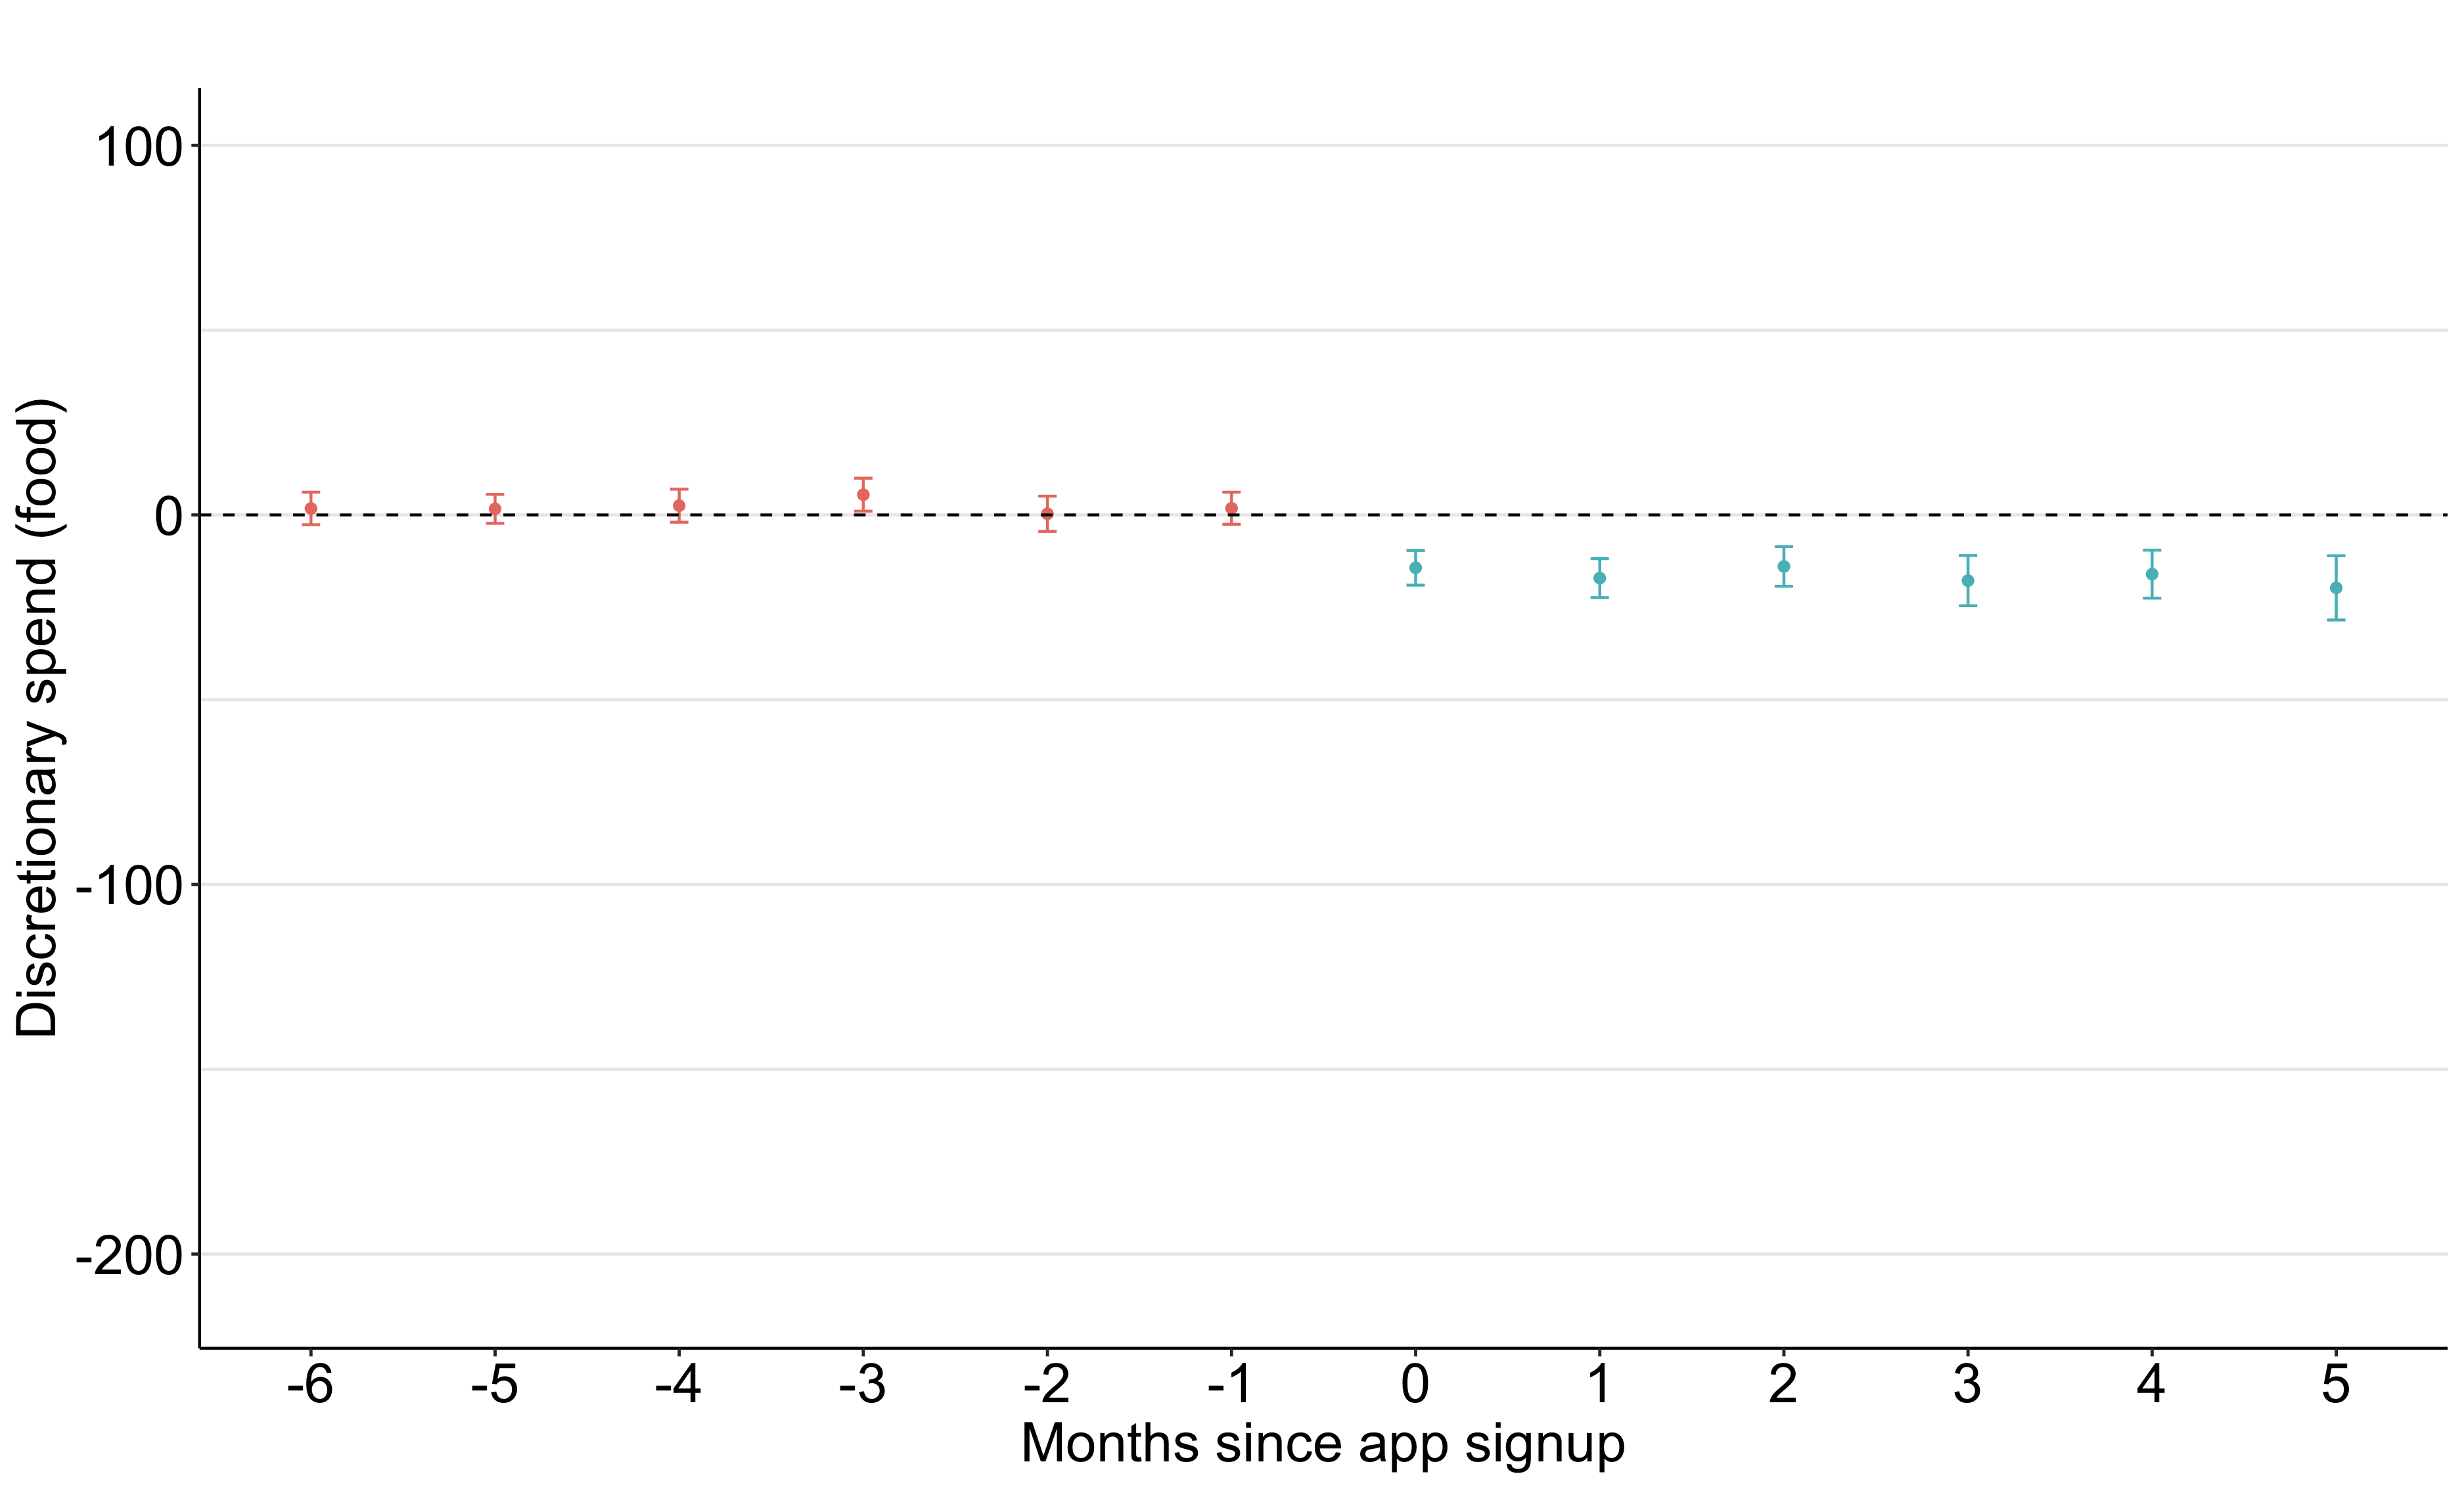
\includegraphics[width=.49\textwidth]{\figdir/disag_dspend_food_cond_es.png}
    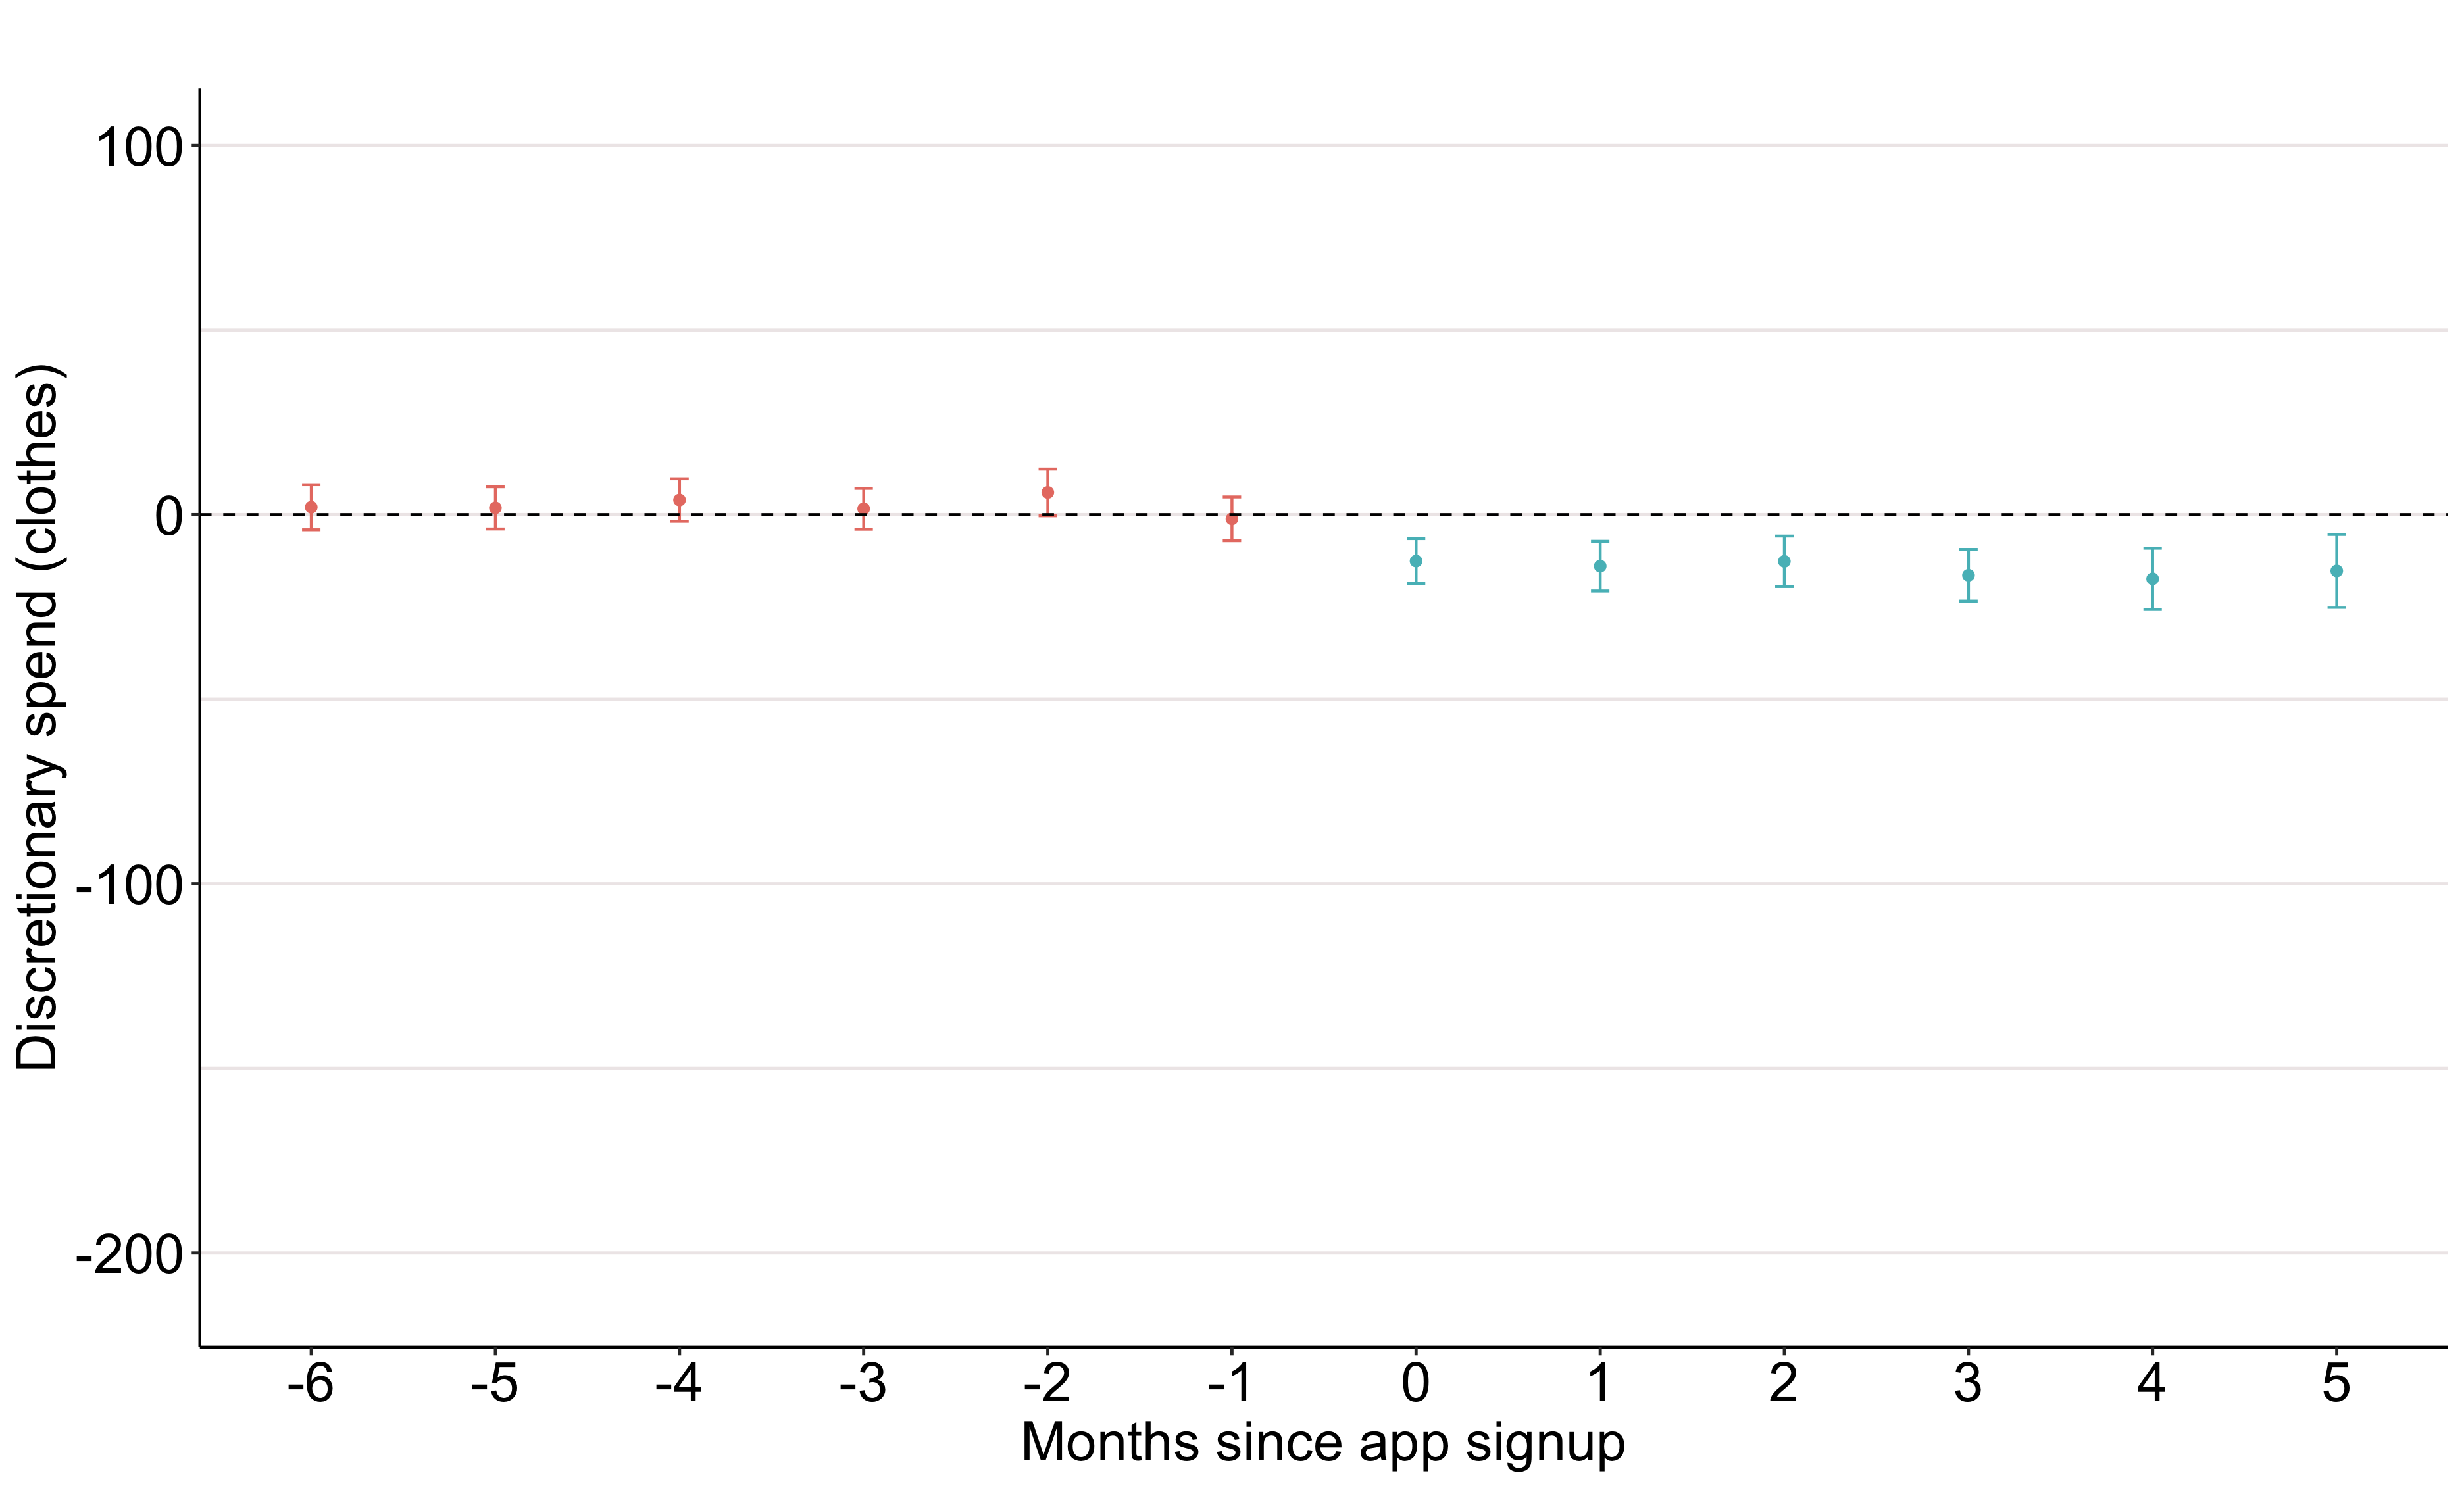
\includegraphics[width=.49\textwidth]{\figdir/disag_dspend_clothes_cond_es.png}
    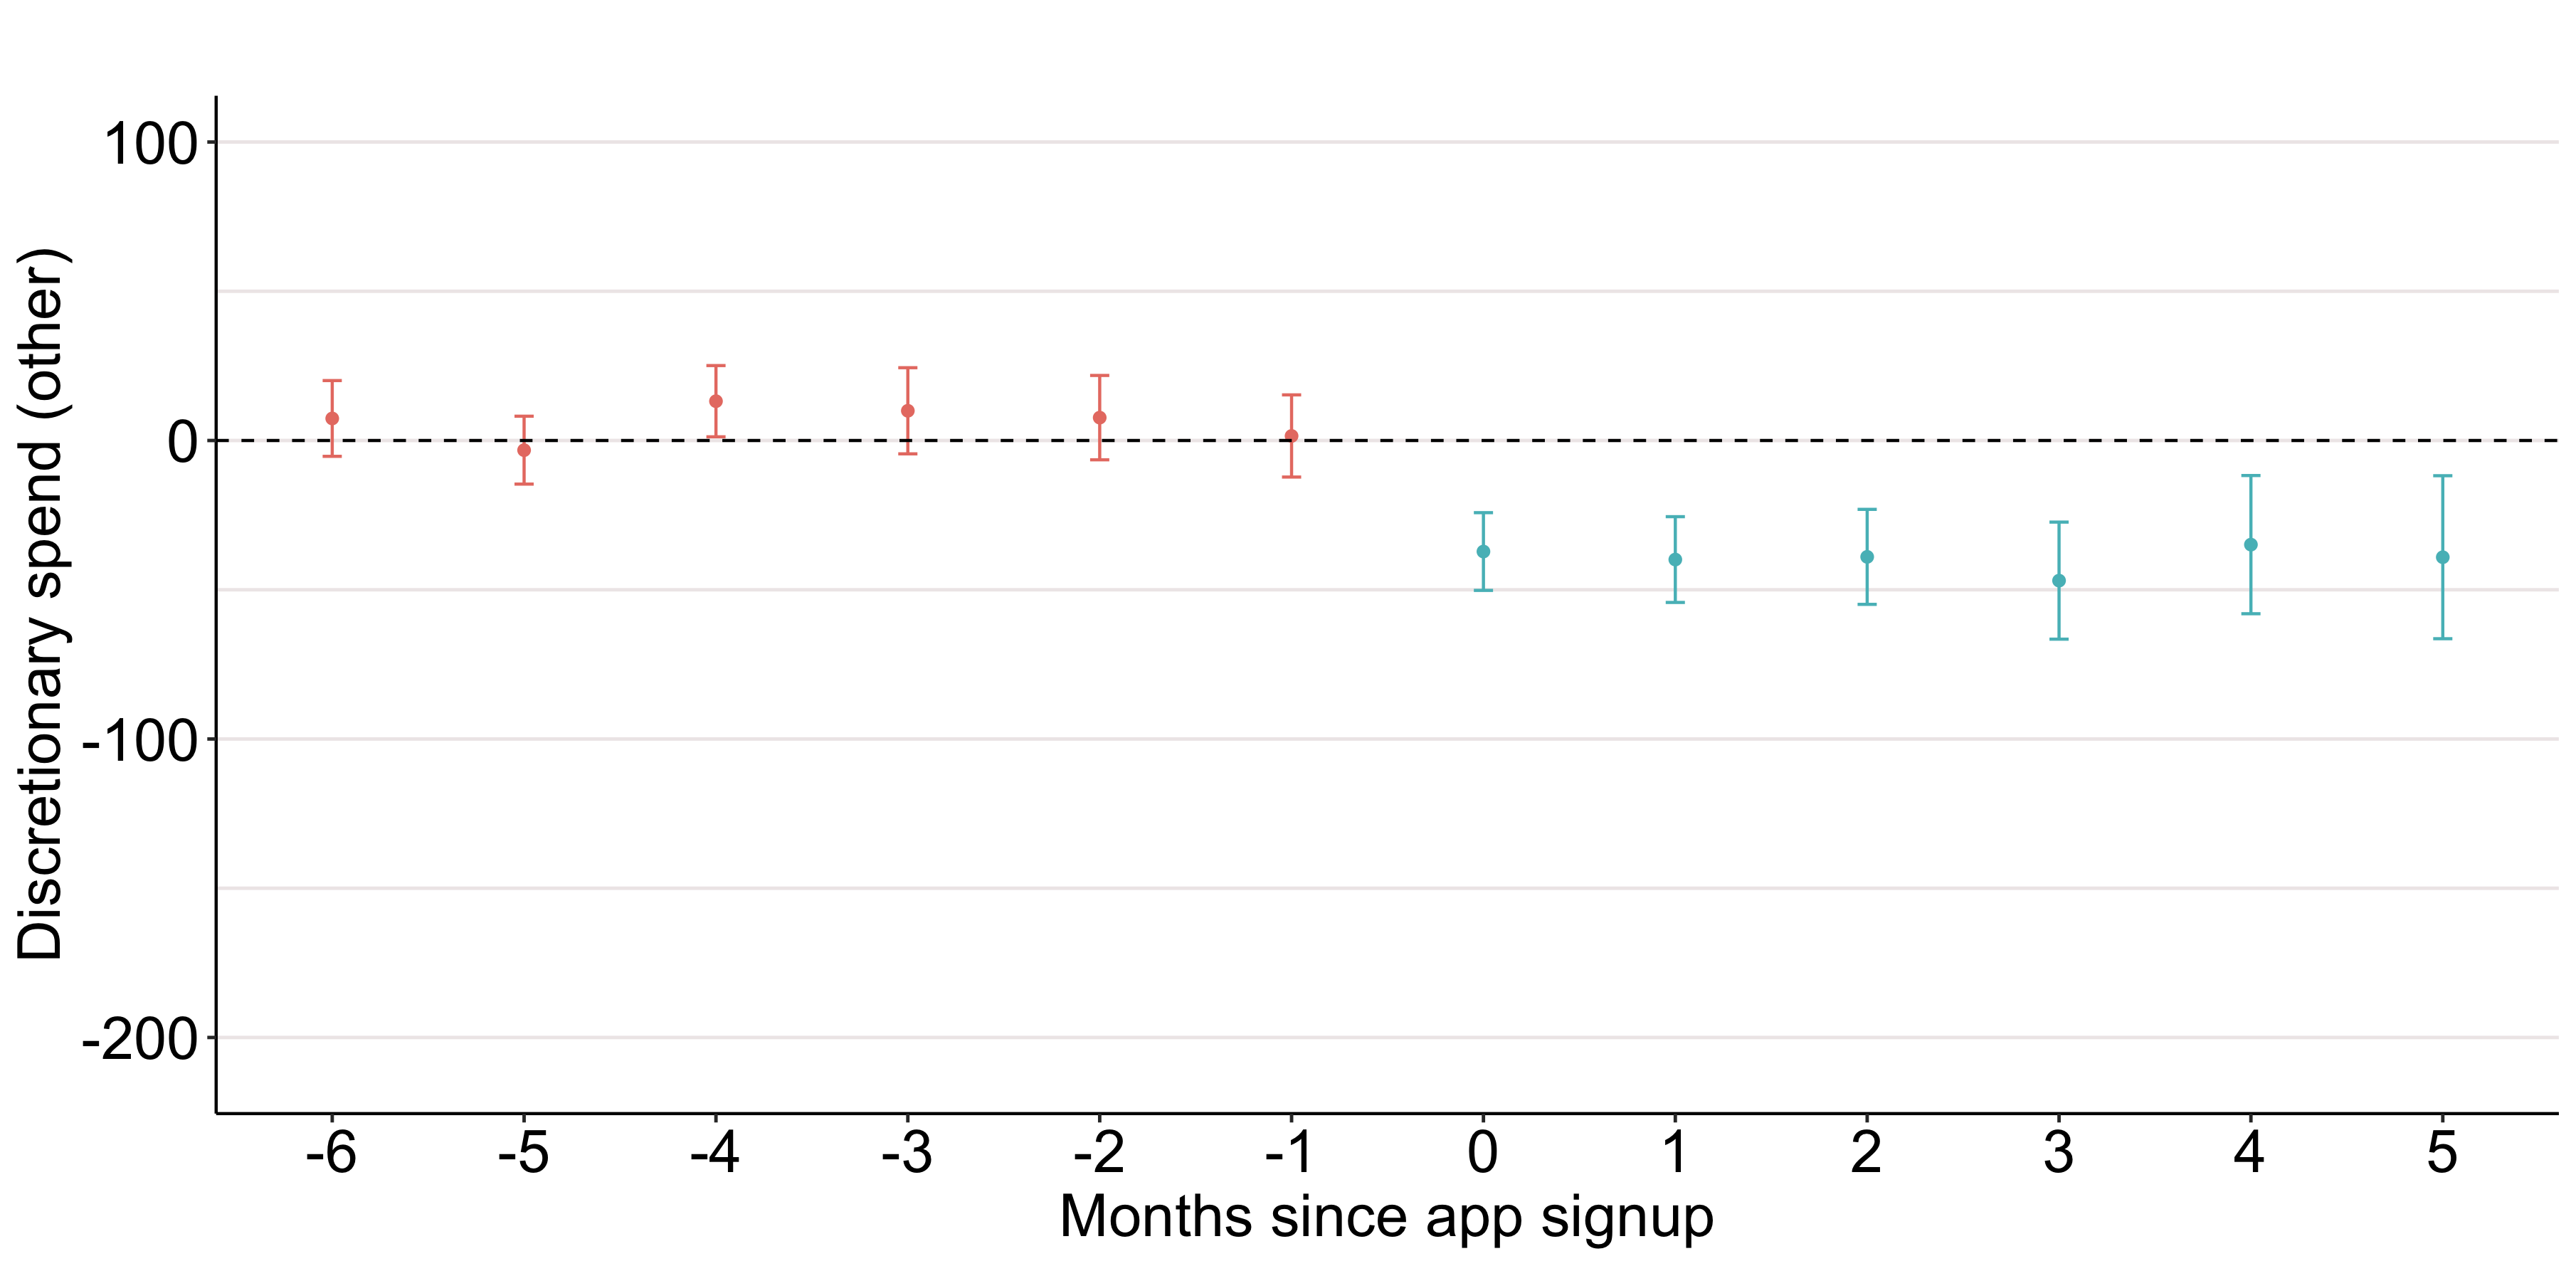
\includegraphics[width=.49\textwidth]{\figdir/disag_dspend_other_cond_es.png}
    \fignote{\textwidth}{Effect of app use on total discretionary spend (for
        reference) and its subgroups. Point estimates represent
        group-time average treatment effects aggregated to periods since
        treatment exposure, as defined in Section~\ref{sub:estimation}. Red
        lines represent point estimates and uniform 95\% confidence bands for
        pre-treatment periods allowing for clustering at the user level. If the
        null hypothesis that parallel trends hold in all periods is correct,
        these should be equal to zero. Blue lines provide similar information
    for post-treatment periods.}
\end{figure}



